\documentclass[a4paper]{article}
\usepackage[utf8]{inputenc}
\usepackage{float}
\usepackage{svg}
\usepackage{titlesec}
\usepackage{graphicx}
\usepackage[hmargin=1.4in, vmargin={1.4in,1.4in}]{geometry}


% \graphicspath{ {./img/} }

% \usepackage{xpatch}
% \xpatchcmd{\thebibliography}{\section*}{\section}{}{}

\usepackage[colorlinks,
            linkcolor=red,
            anchorcolor=blue,
            citecolor=red]{hyperref}

\usepackage{fancyhdr}

\pagestyle{fancy}
\fancyhf{}
% \fancyhead[L]{\textsl{\rightmark}}
\fancyhead[R]{\textsl{\rightmark}}
\fancyfoot[R]{\textbf{\thepage}}
\renewcommand{\headrulewidth}{0pt}
            
\usepackage{graphicx}
\usepackage{subfigure}
\usepackage{amsthm}
\newtheorem{defin}{Definition}[section]
\newtheorem{algor}{Algorithm}[section]
\usepackage{amsmath}
\usepackage{chngcntr}
\numberwithin{figure}{section}
\numberwithin{table}{section}
\usepackage{tabularx}
\usepackage{booktabs}
\usepackage{multirow}
\usepackage[english]{babel}
\usepackage{microtype}
\usepackage{caption}
\usepackage[section]{placeins}
\setcounter{tocdepth}{2}
%========================code
\usepackage{listings}
\usepackage{color}
% \lstset{frame=Trbl,numbers=left,breaklines=true, basicstyle=\footnotesize\ttfamily}
% \usepackage{courier}

\usepackage{minted}
% ===================================================
% \renewcommand{\thesection}{\arabic{section}.}
% \renewcommand{\thesubsection}{\thesection\arabic{subsection}.}
\renewcommand{\thefigure}{\arabic{section}.\arabic{figure}}
\renewcommand{\thesubfigure}{\thefigure(\alph{subfigure})}
\makeatletter
\renewcommand{\p@subfigure}{}
\renewcommand{\@thesubfigure}{(\alph{subfigure})\hskip\subfiglabelskip}
\makeatother

\newenvironment{code}{\captionsetup{type=listing}}{}
% \usepackage{tocbibind}
\usepackage[toc,page]{appendix}


\title{Neural Network for Bisimulation}
\author{Chao Xiang}
\date{April 2019}

\begin{document}
\counterwithin{lstlisting}{section}
\counterwithin{listing}{section}
% \pagestyle{pageHeader}
\maketitle
% \newpage

% \section*{Abstract}
% % A one-page summary of the project as a whole. This MUST be included for all projects.

\begin{abstract}
Neural Network is widely used in many fields.
And it has shown the ability to solve complex problems.
In addition, bisimulation is a very important logical concept.
This project is aiming to explore the capability of the neural network to understand this concept.
The project is divided into three parts.
In the first part, standard bisimulation algorithm was developed.
And one test case generator that can generate random graphs pairs with bisimulation flag is also developed base on the standard bisimulation.
In the second part, a simple neural network was developed to recognise bisimulation.
In the third part, a wide experiment and a deep experiment were done.
The wide experiment tests the performance of the neural network on the graphs of different density.
The result shows that the network performance well and show similarity in most of the cases.
It indicates the representativeness of the test cases produced by the developed random test case generator.
The deep experiment explores the limitation of the network by training the network in the large scale graphs pairs.
The result shows a good ability to understanding the bisimulation. 
However, for some larger scale graphs pairs, the network shows an unusually good performance.
It is speculated coursed by the small size of data set compare with the massive amount of possible graph pairs.
And more experiments still needed.
\end{abstract}
\newpage
\tableofcontents
\newpage
\section{Introduction}
% This will give a brief overview of the project including

% What problem is addressed by the project?
% What are the aims and objectives of the project?
% What are the challenges of the project?
% What is the solution produced?
% How effective is the solution / how successful has the project been?

Artificial Neural Networks (ANNs) has been widely used in multiple areas. 
It has been proved that ANN is Turing complete \cite{siegelmann1995computational}. 
It indicates that understanding the logic (i.e. symbolic computation) is possible theoretically, gives broad application prospects.
There are ANNs \cite{holldobler1999approximating, Holldobler91towardsa} which are able to mimic some first-order logic program. 
However, these solutions were based on the Recurrent Neural Network (RNN) and tried to simulate the logic program rather than catch the logic feature. 
Trying to explore the limitation of ANNs for understanding logical concepts, will help the research of neuro-symbolic integration.

Thus, here we are concerned with the capability of different  Multilayer Perceptrons (MLPs) to understand the logic concept (i.e. bisimulation of logic structures ). 
And MLPs here is introduced as the representative of ANNs, as it is recognised as the original and most basic model of ANNs.
Datasets used to train the MLPs is consisted of groups of generated graphs with flags (i.e. a number that indicates if two graphs are bisimulation).
Then test if MLPs are able to learn the ability to distinguish the bisimulation equivalence.
The report is structured as follows.
First, in Section \ref{sec:background}, relevant research of bisimulation and relation between neural network and logic will be given. 
The specification of the problem and the approach used to explore the limitation will be explained in Section \ref{sec:description}.
Then in Section \ref{sec:relisation}, the process of realisation including component test and the process of the project will be stated.
Section \ref{sec:experiment} will discuss the entire process of the experiments including the setting up, impelementation and analysation of result.
And Section \ref{sec:evaluation}, the summary and the evaluation from the aspect of engineer and research will be explained.
Knowledge and skills gained will be talked in Section \ref{sec:learning}.
The professional issue will be discussed in Section \ref{sec:profession}.
At last the full code of the project, part of the data, screenshots of sample runs, user manual, progress log and Gantt chart will be appended in the Section \ref{sec:appendics}.
\section{Background}
\label{sec:background}
% This will give all the background of the project including

% Background of the problem to be solved.
% Existing solutions/approaches to the problem, if any exist, and a comparison with the solution produced in the project.
% Reading and research done to understand existing approaches, acquire the necessary information and skills to carry out the project.
% A clear statement of the project requirements.
% References to all sources consulted are expected.

This section recalls some notions used in the project with relevant researches.
The notion of \emph{Bisimulation} is introduced as the target logic feature that needs to be learned.
The notion of \emph{Artificial Neural Networks} is introduced as the object that studied in the project.

%==================

\subsection{Bisimulation}\label{sec:bac:bis}
Bisimulation is an important concept. 
It has been introduced in many different fields and plays a very important role.
In modal logic, it was discovered when researches started to study the expressiveness for the logic, in 1970 \cite{Sangiorgi2009}.
Then that was developed by Van Benthem \cite{VanBenthem1976} who came up with \emph{p-relation} that define a symmetric directional relationship between models, i.e. bisimulation.
In computer science, the concept was introduced by Milner while studying concurrency theory \cite{Milner1990}.
The notation was developed to test the equivalence of processes in Calculus of Communication System \cite{Park1981}.
In the set Theory, it was used to determine if the equal objects can be identified with certain model \cite{Sangiorgi2009}.
Also, in formal verification, while describing a system, bisimulation was used to minimise the space of states \cite{Roscoe1994}.

Some of the past solutions for the bisimulation problem is from the perspective of the set theory.
One approach to this problem was studied by Kanellakis and Smolka while studying the equivalence testing of the calculus of communicating systems expression \cite{Milner1980}.
Originally they designed the algorithm to test the equivalence called congruence of finite state processes in CCS \cite{Paige1987}.
The algorithm was given with $O(mn)$ in time and $O(m+n)$ in space.
Another approach was given by Paige and Tarjan \cite{Paige1987}.
They converted the problem as relational coarsest partition problem.
By refining with respect to old blocks rather than current blocks, they reduce the running time into $O(m\log n)$.
Both of them did not solve the problem directly. 
By using a group of reasoning on different perspectives, they convert the problem into a clear and easier problem. 
In this project, the learning algorithm will base on the work of \cite{Paige1987}.

For the first part of the project, the baseline algorithm will use the algorithm based on the set theory. 
In the algorithm, one logical is regarded as a \emph{non-well-founded set}. 
``Such a set has an infinite descending membership sequence" i.e. the elements of the set recursively consisting itself \cite{Aczel}.
Mathematically, in this part the multi-directed graph (logic structure) $G = \langle N, E \rangle$ is regarded as a group of sets where each set represents a \emph{accessible pointed graphs}.
Edges resents membership, that is edge $\langle m, n \rangle$ (also $m \rightarrow n$) means that node $m$ has node $n$ as a element (also $n \in m$).
Then naturally, these sets will be \emph{non-well-founded sets}.
Thus extensionality axiom (two objects are equal if and only if they contain the same elements) cannot be used to define the bisimulation, since these sets may lead to cyclic arguments.
In this project, the baseline algorithm will base on the definition from \cite{Dovier2004}.
\begin{defin}
Given two graphs $G_1=\langle N_1, E_1 \rangle$ and $G_2=\langle N_2, E_2 \rangle$, a bisimulation between $G_1$ and $G_2$ is a relation $b\subseteq N_1 \times N_2$ such that
\renewcommand{\labelenumi}{\arabic{enumi})}
\begin{enumerate}
    \item $u_1b u_2 \wedge \langle u_1, v_1 \rangle \in E_1 \Rightarrow \exists v_2 \in N_2(v_1b v_2 \wedge \langle u_2, v_2 \rangle \in E_2)$
    \item $u_1b u_2 \wedge \langle u_2, v_2 \rangle \in E_2 \Rightarrow \exists v_2 \in N_2(v_1b v_2 \wedge \langle u_1, v_1 \rangle \in E_1)$
\end{enumerate}
\end{defin}
Also, for understanding purpose, a more common definition from the perspective of Kripke model \cite{Glabbeek2011} is given.
Here the multi-directed graph (logic structure) are labelled transition system (LTS), denoted as $(S, \rightarrow, \models)$ with the set of actions $A$ and the set of predicates $P$. $S$ stands for a class of states, $\rightarrow$ stands for a collection of binary relations $\stackrel{a}{\rightarrow}\subseteq S\times S$ where $a \in A$. 
And $\models \subseteq S \times P$, where $s\models p$ indicate that predicate $p \in P$ holds in state $s \in S$ \cite{Glabbeek2011}. Definition in this prospect is given below \cite{Glabbeek2011}.
\begin{defin}
Let $(S, \rightarrow, \models)$ be an LTS over $A$ and $P$. A bisimulation is a binary relation $R \subseteq S \times S$, satisfying:
\renewcommand{\labelenumi}{\arabic{enumi})}
\begin{enumerate}
    \item if $sRt$, then $s \models p \leftrightarrow t \models p$ for all $p\in P$.
    \item if $sRt$ and $s \stackrel{a}{\rightarrow}s'$ with $a \in A$, then there exists a $t'$ with $t \stackrel{a}{\rightarrow} t'$ and $s'Rt'$
    \item if $sRt$ and $t \stackrel{a}{\rightarrow} t'$ with $a\in A$, then there exists an $s'$ with $s \stackrel{a}{\rightarrow}s'$ and $s'Rt'$
\end{enumerate}
\end{defin}

%======================

\subsection{Artificial Neural Networks (ANNs)}
For the second part of the project, the capability of the MLPs for catching the bisimulation equivalence is explored. 
Here MLPs is chosen as the representative of ANNs as a kind for machine learning methods.
Generally, machine learning can be defined as an experience-base computational method \cite{Mohri2013}.
Mohri pointed out that machine learning is mainly used in the classification, regression, ranking, clustering and dimensionality reduction \cite{Mohri2013}.
Among all the machine learning methods ANN is a unique architecture which is good at the pattern related problems \cite{Dayhoff1990}.
This architecture is inspired by the neural cell in the brain. 
By simulate neural cell, a neural network is prospected to learn from experience also understand the logic concepts. 
In 1943, McCulloch and Pitts carried out the first neural network, namely the McCulloch-Pitts Neuron \cite{Dayhoff1990}. 
It is a binary discrete-time element with excitatory, that comes to the perception which can learn the patterns through supervised learning.
And for multilayer perceptron (MLP), it is a feed forward artificial neural network.
A MLP has an input layer, an output layer and at least one hidden layer \cite{rosenblatt1961principles} (See Fiture \ref{fig:mlp}).
More importantly, most ANNs are developed base on the MLP.

\begin{figure}[h]
    \centering
    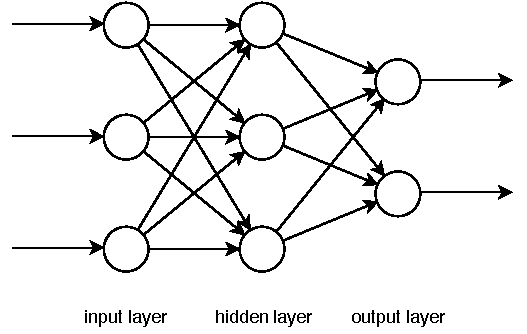
\includegraphics[width=0.5\textwidth]{img/eg_mlp.pdf}
    \caption{Typical MLP}
    \label{fig:mlp}
\end{figure}

While research on logic and ANN has been studied. 
Logic or symbolic system is more expressive and more readable for human. 
Learning base on a symbolic system has less dependence on data.
While commonly, the neural network is known as a less formal system short at human reasoning.
Thus, neuro-symbolic integration is growing rapidly.
It has been shown that feedforward connectionist networks are able to compute certain semantics operators in positional logic programs and approximate them in first-order logic \cite{HITZLER2004245}.
Also, there are scholars constructed recurrent connectionist networks that can approximate logic program and its semantics \cite{holldobler1999approximating, Holldobler91towardsa}.
Further, for the logic relation, a system PAN who accept symbolic input as the condition of the logical rule is developed \cite{guillame2010first}.
There are also research investigates the neural network approach for the first-order abductive inference\cite{Ray_aneural}.

However, this project will focus on MLP and bisimulation only.
Because MLP is the most typical neural network and is part of many neural networks.
By study, the capability, the compute ability of MLPs with certain depth will be evaluated.

% TODO: activation function 

% \subsection{Library Used}
% TODO
% \subsection{Cloud Computing}
% TODO
\section{Problem and Approach}
\label{sec:description}

Here we will give a specification of the problem, and a detailed approach (i.e. the design of solution).
In order to simplify the problem and keep MLPs as simple as possible, one MLP will be used to check only the graphs (models) with a certain number of nodes and certain types of edges.
In other words, each type of graph will have its own MLP.
Notice that all the MLPs will have the same overall architecture.
The only difference will be the number of nodes at each layer.
That is only the bisimulation between graphs with the same scale will be studied.
The problem of the project become that if an MLP is possible to compute the bisimulation equivalence of two same scale models and how well it can do.
The basic steps of approach are as follows.
\begin{itemize}
    \item Generate a standard distinguishing algorithm.
    \item Based on the standard algorithm, develop a dataset generator.
    \item Construct MLPs that can accept graphs pairs and output judgement.
    \item Do experiments on the performance of the MLP with different training sets. \footnote{N.B. this step will be stated independently in Section \ref{sec:experiment}}
\end{itemize}


\subsection{Standard Bisimulation Algorithm}
For the first step, we will directly use the algorithm that solves the \emph{relational coarsest partition problem} \cite{Paige1987}, i.e. given the relation $E$ and initial partition $P$ over a set $U$ find the partition $P$ that \textquotedblleft every other stable partition is a refinement of it \textquotedblright.
From the perspective of set-theory, it is the same as solving bisimulation equivalence \cite{Dovier2004}.
Namely, if each block of the relational coarsest partition of the union of two graphs has nodes from both multi-directed graphs, these two graphs are bisimilar (see the set-perspective definition in Section \ref{sec:background}).
Moreover, compared with the algorithm given by Kanellakis and Smolka \cite{Milner1980}, their algorithm is more efficient in time (see Section \ref{sec:bac:bis}).
Yet, the algorithm given by Paige and Tarjan is not designed for multi-directed graphs.
It only processes the directed graph with only one kind of edges.
So by replacing every operation on one relation by a group of operations on each relation (see Step \ref{each_relation} in Algorithm \ref{alg:sbs}), the algorithm can be used for multi-directed graphs.
Here we give the description of the algorithm based on \cite{Paige1987}.

\begin{algor}\label{alg:sbs}
Standard Bisimulation Algorithm
\begin{enumerate}
    \item Get the union of two given graphs $U$.
    \item Initialise the partition $X$ and block set $C$, where $X=C=\{U\}$.
    \item Get the initial partition $Q$, by refine the only block $U$ in $Q$ with respect to $U$ itself. In other words, split $U$ on the preimage of itself, i.e. $Q = \{E^{-1}(U), U-E^{-1}(U)\}$, where $E$ is the any type of binary relation of nodes (also edges).
    \item Loop until block set $C$ is empty.
    \begin{enumerate}
        \item \label{loop} Pop the first block $s$ from block set $C$
        \item Check first two blocks of partition $Q$, that is contained in block $s$, make block $b$ be the smaller one.
        \item In partition $X$ split the block $s$ into block $b$ and block $s'=s-b$. if $s'$ is compound with respect to partition $Q$, add it back to block set $C$
        \item \label{each_relation} For each type of relation $E_i$, i.e. $i=1, i=2$ if there are two types of edges.
        Refine every blocks in partition $Q$ with respect to block $b$ and block $s'$.
        \item Add all blocks $x\in X$ that are compound with respect to partition $Q$ to block set $C$
    \end{enumerate}
    \item If there are nodes of both graphs in each block of partition $Q$ return true, else return false.
\end{enumerate}

\end{algor}

% \begin{defin}
% Concepts used in the algorithm. \footnote{All the definition here directly from \cite{Paige1987}}

% \begin{itemize}
%     \item $U$ is the union of two given graphs.
%     \item $S$ is the subset of $U$, i.e. $S \subseteq U$
%     \item $E$ is the links of $U$, which means edge $\langle x, y \rangle \in E $ (also denoted $xEy$).
%     \item For any subset $S$, $E(S) = \{y|\exists x \in S \text{ such that } xEy\}$ and $E^{-1}(S)=\{x|\exists y\in S \text{ such that } xEy \}$
%     \item If $B \subseteq U$, $B$ is \emph{stable} with respect to $S$ if either $S\subseteq E^{-1}(S)$ or $B\cap E^{-1}(S)=\emptyset$
%     \item If $P$ is a partition of $U$, $P$ is \emph{stable} with the respect to $S$ if all of the blocks belonging to $P$ are stable with respect to $S$.
%     \item $P$ is \emph{stable} if it is stable with respect to each of its own block.
% \end{itemize}
% \end{defin}
% This algorithm keep refine the a partition $Q$ (with the initial state that only contain $U$) until it is \emph{stable}.


\subsection{Test Case Generator}\label{sec:generator ds}
All the data used in this project is self-generated random and abstract without any human participation.
Here the model (multi-directed graph) generated will be represented as an expend adjacency matrix (see Figure \ref{fig:exp:model_represent}), where 1 stands for existence.
\begin{figure}[h]
    \centering
    \subfigure[Model]{
        \label{fig:example1_model}
        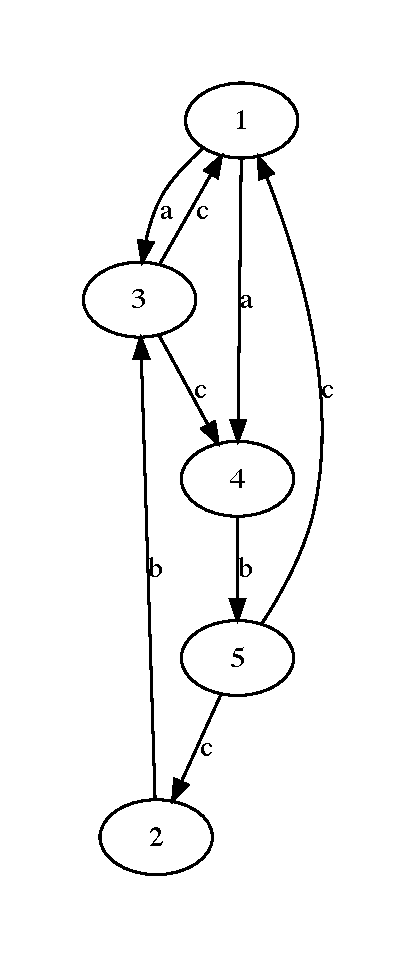
\includegraphics[width=2.0cm]{img/graph_example.pdf}}
    \subfigure[Adjacency Matrix]{
        \label{fig:example1_matrix}
        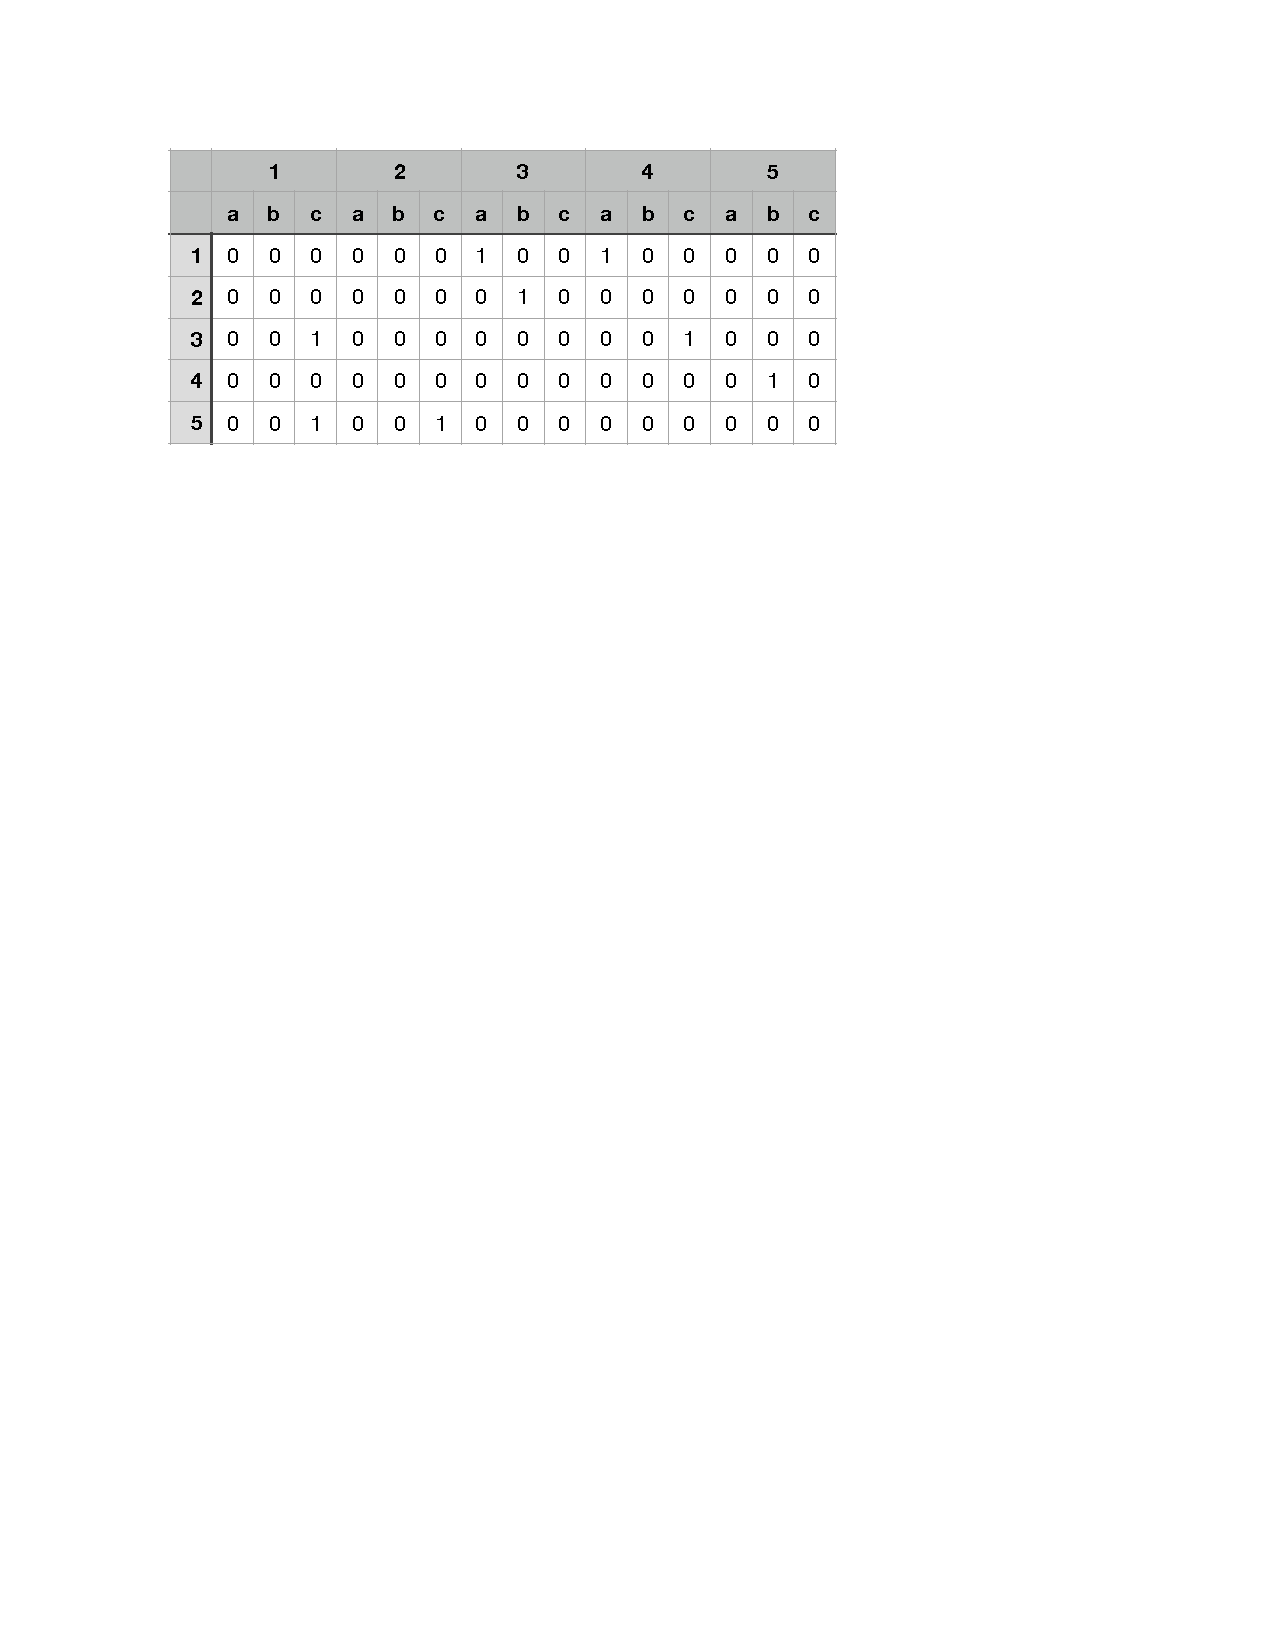
\includegraphics[width=0.6\textwidth]{img/example1_matrix.pdf}}
    \caption{Example model represent}
    \label{fig:exp:model_represent}
\end{figure}

There are two generators implemented.
However, only one is used in the final experiments (to be explained in Section \ref{sec:relisation})
The first idea is to randomly generate graphs.
Depends on the rate given, generate a bisimilar graph of another random non-bisimilar graph.
Then record them into the appointed file with flags.
Description of this algorithm is given as follow.
\begin{algor}
\label{alg:R_tcg}
Random Test Case Generator
\begin{enumerate}
    \item \label{item:gen_ran}Generate a random graph with certain scale, using the given density times a random number ($< 1$, $> 0$) as a probability of each possible edge.
    \item According given rate of positive cases and negative cases, decide to generate a bisimilar graph (jump to Step \ref{item:bi}) or non-bisimilar graph (jump to Step \ref{item:non_bi}).
    \item \label{item:non_bi} Keep generate random graph like Step \ref{item:gen_ran} and check the bisimulation equivence, until they are not (then jump to Step \ref{item:convert}).
    
    \item \label{item:bi}Get the \emph{relational coarsest partition} $P_\text{origin}$ of given graph.
    \item Randomly divides the nodes of the new graph into the same partition $P_\text{similar}$, i.e. the partition that has the same number of blocks (N.B. the length of each block not necessary to be same).
    \item Assemble the minimum bisimilar graph, where each block of its partition contains only one node. 
    \item \label{item:bi_end}For each edge of the minimum graph, generate a random number ($\geq 1$) of edges between the random nodes from two corresponding blocks of $P_\text{similar}$ respectively.
    
    \item \label{item:convert}Convert the new generated graph into adjacency matrix.
    \item Write two graphs with flag into file (jump to Step \ref{item:gen_ran} if there are not enough test cases).
\end{enumerate}
\end{algor}

However, the test cases generated may not actually random, which may have some superficial features that are easy to be caught by the later MLP (to be described in Section \ref{sec:des:ml}).
For example the heuristic algorithm for generate bisimilar graph (see Algorithm \ref{alg:R_tcg}, Step \ref{item:bi} to Step \ref{item:bi_end}) may have some kind of inclination.
To get rid of these potential bias, a full case generator is designed.
This generator can generate all possible graphs in given scale and record all possible combinations with flags.
The basic idea of iteration is that since a graph can be seen as an adjacency matrix, it can be represented as a binary string.
By counting in binary, all possible graphs on the same scale can be traversed.
Here gives the description of this algorithm.
\begin{algor}
\label{alg:F_tcg}
Full Test Case Generator
\begin{enumerate}
    \item For every graph, calculate its minimum bisimilar graph. Meanwhile, construct a dictionary where the key is the minimum bisimilar graph and the value is a set of all graphs that are bisimilar, i.e. have the same minimum bisimilar graph which is their key.
    \item According to the dictionary, catalogue all the graph (graphs with the same key will have the same label).
    \item Go through all graphs again, generate all combinations with flag base on their label.
\end{enumerate}
\end{algor}

\subsection{MLP Structure}
\label{sec:des:ml}
After the test case generator produces data, the network should be trained.
The structure is designed to be as simple as possible.
Combine with the process step of the standard algorithm, the network is structured to meet the process (see Figure \ref{fig:mlp_model}).
The first layer is the input layer, which will accept fixed length binary (i.e. adjacency matrix).
In order to push the network to get the abstraction, the second layer called re-represent layer has fewer neurons than the input layer. 
And the first two layers are divided into two independent parts that share parameters (see Part 1 and Part 2 in Figure \ref{fig:mlp_model}).
Each part will accept one graph.
The distinguishing part will accept input from two graphs and get the conclusion about bisimulation equivalence, i.e. output the probability of positive and negative.
There are three reasons to design a network like that.
First is by sharing the parameters, the overall training will be master.
The second reason is that it solves the problem of sequence, i.e. the output will not be affected by the priority of two graphs.
The third reason is that this kind of modular design will be much easier for reuse, e.g. used as part of the graph simplify the network.

\begin{figure}[h]
    \centering
    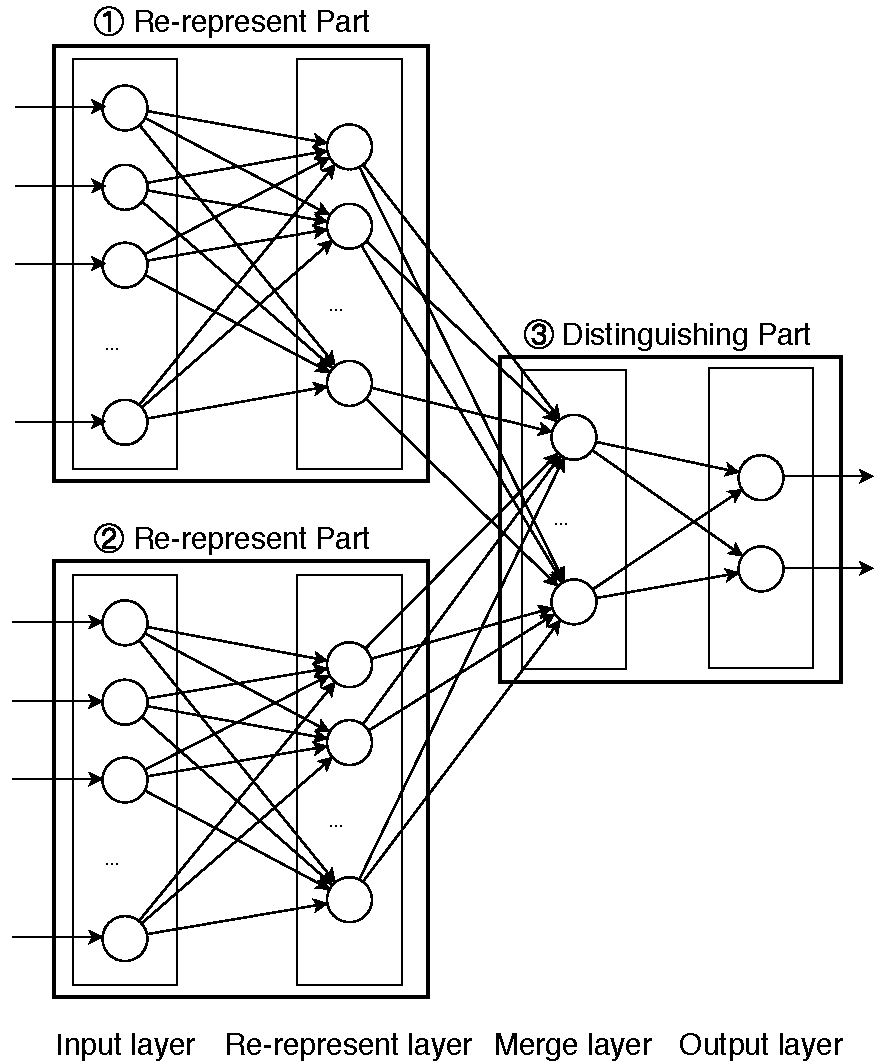
\includegraphics[width=0.65\textwidth]{img/mlp.pdf}
    \caption{MLP model}
    \label{fig:mlp_model}
\end{figure}

\subsection{General Structure}
The design of the general structure is aimed at developing a reusable tool.
Thus the structure is very simple and highly modularised (see Figure \ref{fig:general_str}).
Dataset generator and ML-algorithm is packed independently.
And each module can be called in a python program or used as a command line tool directly by the user.
\begin{figure}[h]
    \centering
    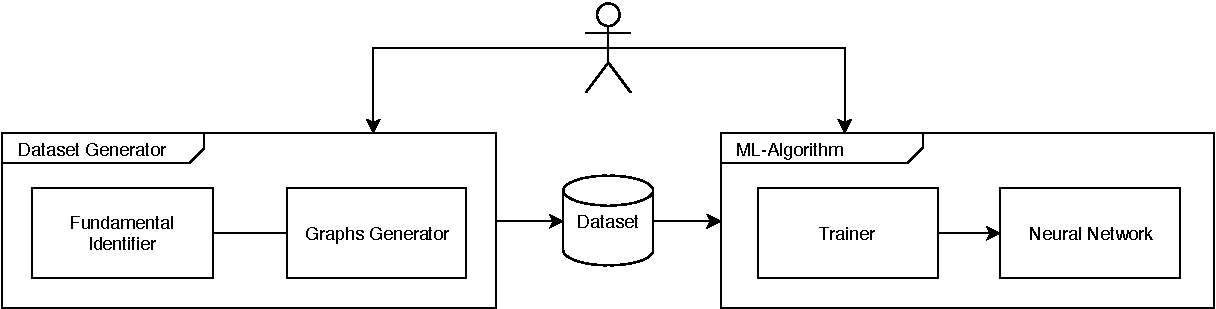
\includegraphics[width=\textwidth]{img/architecture.pdf}
    \caption{General structure}
    \label{fig:general_str}
\end{figure}


% \section{Design}
\label{sec:design}
% This will give a description of the design.

% The organisation of this section should be the same as for the design documentation, and full details of the design are required. Typically it will comprise
    % a description of the anticipated components of the system and how they are to be organised;
    % a description of data structures used by the system;
    % algorithms to manipulate these data structures;
    % a design of the intended interfaces.
% Depending on the project and approach used, the followings are expected (refer to the guideline of the design stage for details):
    % Object-oriented design methodology:
    % Use-case diagrams; An interaction chart; The objects to be used in the system; Attributes and methods of objects; Pseudo-code for the key methods; Interface design.
    % Traditional design methodology:
    % Data dictionaries; System boundary diagrams; Entity-relationship diagrams; Logical table structures; Physical table structures; Transaction matrix; Pseudo-code for the key methods; Interface design.
    % Empirical investigation of hypothesis: in addition, the following is expected
    % A statement of the hypotheses to be tested; A description of the test data to be used; An experiment design, the experiments to be performed, any control to be used; A description of how the results will be analysed, including any statistical techniques that will be used; Anticipated conclusions.
    % Devising new algorithms: in addition, the following is expected
    % A description of the approach used to solve the problem; A description of how the new algorithms will be analysed, including mathematical and experimental analysis.
% All design documentation, representing the final design used on the project should be supplied.
% Any modifications made to the design presented in the design documentation and presentation should be stated and justified. ***

% It is often best to include the full details of the design as an appendix. In such a case, the design chapter in the main part of the project report should only discuss the most important elements of the design to your design report and state clearly what other elements will be given in the appendix.

% Keep in mind that examiners might not look at all the details of the material included in the appendices. So, make sure that the really important points of the design are explained here.

\subsection{Architecture}
Main idea is to generate variable datasets

\begin{figure}[H]
\centering
\caption{Main architecture}
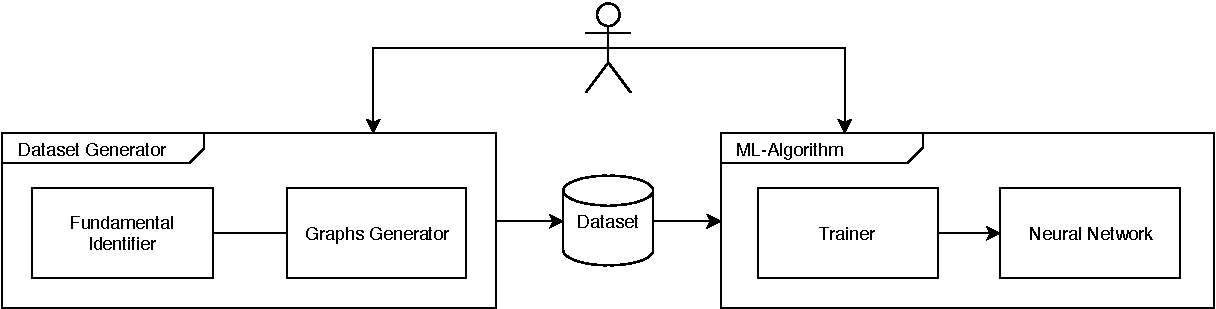
\includegraphics[width=\textwidth]{img/architecture.pdf}
\label{fig:global_performance}
\end{figure}



\subsection{Algorithm Design}
In this project, there are two algorithms involve. 
Both of them is used to check the existence of bisimulation relation between two given graphs.
The first one is a non-machine learning algorithm based on the work of Paige and Tarjan \cite{Paige1987}. 
The second algorithm is a neural network, training on the data that generated by the first algorithm.
\subsubsection{Traditional Bisimulation Algorithm}
Paige and Tarjan give the general solution of relational coarsest partition problem \cite{Paige1987}, which is identical to computing bisimulation equivalence \cite{Dovier2004}.

\section{Realisation}
\label{sec:relisation}
% should mention the data issue

% 4. DATA REQUIRED:
% what data were needed for the project and where it was obtained from;
% ethical use of data, including use of human data & human participants:
    % ethical use of data
        % explicitly specify whether you used
        % Synthetic data,
        % or
        % Real Non Human data
            % explicitly confirm an ethical source of the data,
            % confirm the University or a relevant Professional Body Ethical approval has been obtained for the use of the data in your project.
            % where applicable, include into appendix the University Ethical approval obtained by your 1st supervisor for the project on your behalf.
        % or
        % Real Human data:
            % explicitly confirm an ethical source of the data
            % explicitly confirm that the University Policy on ethical use of human data has been followed: here is the flow chart for the University Ethical approval.
            % explicitly confirm that the University or a relevant Professional Body Ethical approval has been obtained for the use of the data in your project.
            % where applicable, include into appendix the University Ethical approval obtained by your 1st supervisor for the project on your behalf
        % be aware that only the following types of data do not require Research ethics approval:
            % information freely available in the public domain;
            % anonymised records and data sets that exist in the public domain
    % ethical use of human participants (other then project 3rd party evaluation)
        % explicitly state if human participants were involved in the project;
        % if human participants were involved in the project,
            % explicitly confirm that the University ethical procedure has been followed: here is the flow chart for the University Ethical approval;
            % explicitly confirm that the University or a relevant Professional Body Ethical approval has been obtained for the use of human participants in your project;
            % include into appendix human participants information sheet and consent forms completed and signed by the human participants on your project.

% 6. REALISATION
% This will give a description of how the design was implemented and a description of the testing of the implementation. The following is expected:
    % Description of how the design was implemented for each stage and each component of the system.
    % Description of problems encountered during implementation and the solutions to these problems.
    % Changes made to the design in the course of implementation and the justification. ***
    % Description of various testing of the implementation of each stage and each component of the system including test cases used, expected results, and actual results.
    % Snapshot of code listing of key methods and a small number of screen shots may be included. However, typically, full code listings, detail screen shots, and test runs will appear as appendices.

% Again, keep in mind that examiners might not look at all the details of the material included in the appendices. So, make sure that the really important points of the implementation and testing are explained here.

% *** Typically, there are two cases of modifications as compared with the design stage:

    % If the design has been revised since the design stage and the implementation now follows this revised design, the DESIGN section should present the revised design together with comments explaining and justifying the changes.
    % If the design has not been revised since the design stage, but the implementation differs to a lesser or greater extent from that design, the DESIGN section would be pretty much identical to the original design documentation but the REALISATION section would explain the differences between design and implementation.

Implementation is not always the same as the design.
During the realisation of the standard bisimulation algorithm, a visualisation tool for graphs is needed for development. 
It gives the graph an intuitional presentation so that the standard algorithm can be verified much easier.
And the same situation happens in the development of machine learning part.
Follows are the actual structure implemented (see Figure \ref{fig:actual_str}).
\begin{figure}[h]
    \centering
    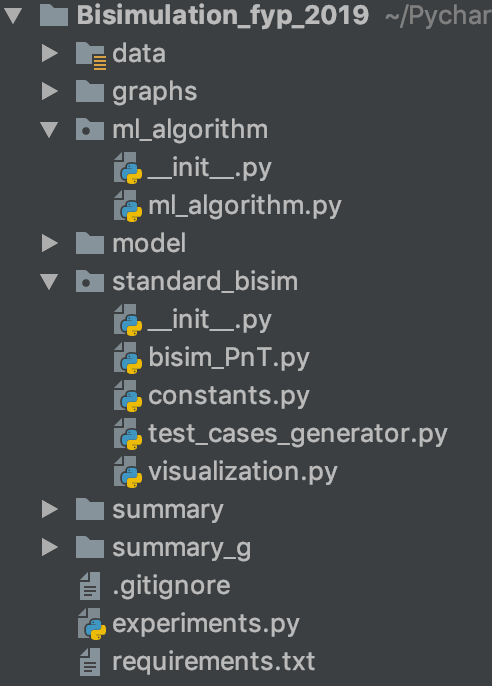
\includegraphics[width=0.4\textwidth]{img/actual_str.png}
    \caption{Actual structure}
    \label{fig:actual_str}
\end{figure}

\begin{description}
    \item[\texttt{/data/}] It is used to store the generated test cases data. They are saved as \texttt{.csv} file and are the output of \texttt{test\char`_cases\char`_generator.py}, the input of \texttt{ml\char`_algorithm.py}.
    
    \item[\texttt{/model/}] This directory is used to store the parameters of trained/half-trained machine learning models. It allowed training resume form break point and also directly apply of trained models.
    Models are save as \texttt{.ckpt} files.
    And during the training, \texttt{ml\char`_algorithm.py} will keep recording the current model.
    
    \item[\texttt{/graphs/}] The graphs figure that been visualised is put in this directory. 
    
    \item[\texttt{/summary/}] It is used to store the summary file generate by \texttt{ml\char`_algorithm.py}. These file record all the metric calculated during the training (i.e. loss, accuracy, precision and recall) for later analyse.
    
    \item[\texttt{/summary\char`_g/}] TensorFlow Graphs generated during the calculation of train are stored here. It can be visualised by the TensorBoard, which will do a great help in the implementation of the neural network.
    
    \item[\texttt{/requirement.txt}] This file is a text file which records all the package needed. An environment can be established easily based on this file.
    
    \item[\texttt{/.gitignore}] The project is managed by the distributed version control system \texttt{Git}. It is a configuration file that will make \texttt{Git} ignore assigned files.
    
    \item[\texttt{/experiments.py}] This file contain the experiments of the proeject, and will described in Section \ref{sec:experiment}.
    
    \item[\texttt{/standard\char`_bisim/}] Under this directory, that are \texttt{bisim\char`_PnT.py}, \texttt{test\char`_cases\char`_generator.py} and \texttt{visualisation.py}. Detail will described below (i.e. Section \ref{sec:comp_imp}). 
    
    \item[\texttt{/ml\char`_algorithm/}] It is used to hold \texttt{ml\char`_algorithm.py}. Detial of this part will be descussed below (i.e. Section \ref{sec:comp_imp}).
    
\end{description}


\subsection{Components Implementation}
\label{sec:comp_imp}
The detailed description of implementation is given in this part.

\subsubsection{Implementation of Standard Bisimulation Algorithm}
The first part of the project is to develop the standard bisimulation algorithm base on the algorithm given in \cite{Paige1987}.
This algorithm is implemented as a class \texttt{BisimPnT}.
Following functions are included.
Also the code listing of \texttt{coarsest\char`_partition() } is given here (See Listing \ref{lst:coarsest part}).\vspace{0.5em}

% \noindent
\begin{center}
\begin{tabularx}{0.9\textwidth}{lX}
    \toprule
    \textbf{Signature}          & \texttt{\char`_\char`_init\char`_\char`_(self, labels, graph\char`_g, graph\char`_h=None)}\\ \midrule
    \textbf{Description}        & Initiate the object. Union the given graphs and record the possible edges (\texttt{labels})\\ \midrule
    \textbf{Return}             & N/A \\ \bottomrule
\end{tabularx}
\end{center}
\begin{center}
\begin{tabularx}{0.9\textwidth}{lX}
    \toprule
    \textbf{Signature}          & \texttt{preimage(self, block\char`_s, label=None)}\\ \midrule
    \textbf{Description}        & Calculate the preimage of block with respect to a given type of edge (also relation). If type asigned, it will compute the preimage without distinguishing the types of edge, i.e. all edges will be seen as same relation (\texttt{label}).\\ \midrule
    \textbf{Return}             & $E^{-1}_{\text{label}}(\text{block\_s})=\{x|\exists y \in \text{block\_b } \text{such that } xE_\text{label}y\}$ \\ \bottomrule
\end{tabularx}
\end{center}
\begin{center}
\begin{tabularx}{0.9\textwidth}{lX}
    \toprule
    \textbf{Signature}          & \texttt{split\char`_block(self, block\char`_b, block\char`_s, label=None)}\\ \midrule
    \textbf{Description}        & Calculate the result of split the \texttt{block\char`_b} with the preimage of \texttt{block\char`_s}. It \texttt{label} is not assigned, then block b will be split with respect to all relation.\\ \midrule
    \textbf{Return}             & $\text{split}(\text{block\_b}, \text{block\_s}) = \{\text{block\_b}\cap E^{-1}_{\text{label}}(\text{block\_s}), \text{block\_b} - E^{-1}_{\text{label}}(\text{block\_s})\}$ \\ \bottomrule
\end{tabularx}
\end{center}
\begin{center}
\begin{tabularx}{0.9\textwidth}{lX}
    \toprule
    \textbf{Signature}          & \texttt{compound\char`_blocks(self, partition\char`_Q, partition\char`_X)}\\ \midrule
    \textbf{Description}        & Check if all the blocks in \texttt{parition\char`_X}, if their are compound or not. Return a set of all compound blocks. \\ \midrule
    \textbf{Return}             & a set of blocks in \texttt{partition\char`_X} that is compound with respect to \texttt{partition\char`_Q} \\ \bottomrule
\end{tabularx}
\end{center}
\begin{center}
\begin{tabularx}{0.9\textwidth}{lX}
    \toprule
    \textbf{Signature}          & \texttt{is\char`_compound\char`_to(self, block\char`_s, partition)}\\ \midrule
    \textbf{Description}        & Check if \texttt{block\char`_s} is compound with respect to \texttt{partition}, i.e. if \texttt{block\char`_s} contain more then one block in \texttt{partition}. \\ \midrule
    \textbf{Return}             & The smaller contained block in \texttt{partition} of \texttt{False} if \texttt{block\char`_s} is simple \\ \bottomrule
\end{tabularx}
\end{center}
\begin{center}
\begin{tabularx}{0.9\textwidth}{lX}
    \toprule
    \textbf{Signature}          & \texttt{coarsest\char`_partition(self, plot=False)}\\ \midrule
    \textbf{Description}        & Calculate the coarsest partition of the graph given when initialisation. \\ \midrule
    \textbf{Return}             & The coarsest partition \\ \bottomrule
\end{tabularx}
\end{center}
\begin{center}
\begin{tabularx}{0.9\textwidth}{lX}
    \toprule
    \textbf{Signature}          & \texttt{get\char`_min\char`_graph(self)}\\ \midrule
    \textbf{Description}        & Assemble a min bisimulation graph.  \\ \midrule
    \textbf{Return}             & The minimum bisimulation graph\\ \bottomrule
\end{tabularx}
\end{center}
\begin{center}
\begin{tabularx}{0.9\textwidth}{lX}
    \toprule
    \textbf{Signature}          & \texttt{is\char`_bisimilar(self)}\\ \midrule
    \textbf{Description}        & Check it two given graph is bisimulation by checking if there are nodes from both graph in each of the coarsest partition. \\ \midrule
    \textbf{Return}             & \texttt{True} or \texttt{False}\\ \bottomrule
\end{tabularx}
\end{center}

% \captionof{listing}{Function calculate coarsest partition \label{lst:coarsest part}}\vspace{-0.6em}
\begin{code}
\caption{Function calculate coarsest partition}
\label{lst:coarsest part}
\begin{minted}[linenos, frame=single,breaklines]{python}
def coarsest_partition(self, plot=False):

    # Step 1 Initial U 
    block_u = set(self.full_graph_U.nodes())
    
    # Step 2
    partition_X = [block_u]
    block_set_C = [block_u]
    
    # Step 3
    partition_Q = self.split_block(block_u, block_u)
    
    # Step 4
    block_set_C = self.compound_blocks(partition_Q, partition_X)
    while len(block_set_C) != 0:
        # Step a:
        # select refining block_b
        # a compound block of partition_X
        block_s = block_set_C.pop()  
        # a block of Q that contained in s
        block_b = self.is_compound_to(block_s, partition_Q)  

        # Step c:
        # update X:
        partition_X.remove(block_s)
        partition_X.append(block_s - block_b)
        partition_X.append(block_b)  # split block S in X

        # if the rest is still not simple, put it back to C
        if self.is_compound_to(block_s - block_b, partition_Q) is not False:
            block_set_C.append(block_s)
        
        # Step d
        for label in self.labels:

            # compute preimage of B
            preimage_b = self.preimage(block_b, label)
            # compute preimage of S - B
            preimage_s_sub_b = self.preimage(block_s - block_b, label)

            # refine Q with respect to B and S-B
            new_partition_Q = []
            for block_d in partition_Q:
                block_d1 = block_d.intersection(preimage_b)
                block_d2 = block_d - block_d1
                block_d11 = block_d1.intersection(preimage_s_sub_b)
                block_d12 = block_d1 - preimage_s_sub_b

                if len(block_d2) and block_d2 not in new_partition_Q:
                    new_partition_Q.append(block_d2)
                if len(block_d11) and block_d11 not in new_partition_Q:
                    new_partition_Q.append(block_d11)
                if len(block_d12) and block_d12 not in new_partition_Q:
                    new_partition_Q.append(block_d12)
                partition_Q = new_partition_Q
        
        # Step 5
        block_set_C = self.compound_blocks(partition_Q, partition_X)
        # if needed visualise the result
        if plot:
            vi.plot_graph_with_partition(self.full_graph_U, partition_Q)

    self.co_partition = partition_Q
    return partition_Q
\end{minted}
\end{code}


However, there is a visualisation tool that can plot the multi-directed graphs (e.g. Figure \ref{fig:example1_model} is drawn by this tool) are developed based on \texttt{graphviz}. 
It can also colour the graph with a given partition.

With this tool, the development and component tests became much easier.
There is one main function below.
\begin{center}
\begin{tabularx}{0.9\textwidth}{lX}
    \toprule
    \textbf{Signature}          & \texttt{plot\char`_graph\char`_with\char`_partition(graph, blocks=None, file\char`_name="test")}\\ \midrule
    \textbf{Description}        & Visualisation the graph with partition and save the image. If no \texttt{blocks} (i.e. partition) given it will output image without colour.\\ \midrule
    \textbf{Return}             & Image file \\ \bottomrule
\end{tabularx}
\end{center}


\subsubsection{Implementation of Test Case Generator}\label{sec:imptestcasegenerator}
It was considered that there are two generators (see Section \ref{sec:generator ds}).
However, during the primary test, the full test generator (see Algorithm \ref{alg:F_tcg}) is too expensive both in computation and space.
Specifically, for the graphs with $n$ node and $m$ types of edges.
Then there are $2^{n*n*m}$ possible graphs.
After combination, there will be $(2^{n^2m}*(2^{n^2m}-1))/2 \approx 2^{2n^2m}$.
If graphs have 3 nodes and 2 types of edges, there will be $2^{36}$ (around 60 billion) test cases.
Thus, it is too expensive for this project.
Instead, we will repeat the experiments in different parameters to minimise the possibles.

Here we give the code about random test case generator described in Algorithm \ref{alg:R_tcg} and the heuristic algorithm for generate bisimilar graph (see Algorithm \ref{alg:R_tcg}, Step \ref{item:bi} to Step \ref{item:bi_end}).
Also, the generator is packed as a command line tool for the convenience of further use (see Figure \ref{fig:arggenerator}).
\begin{figure}[h]
    \centering
    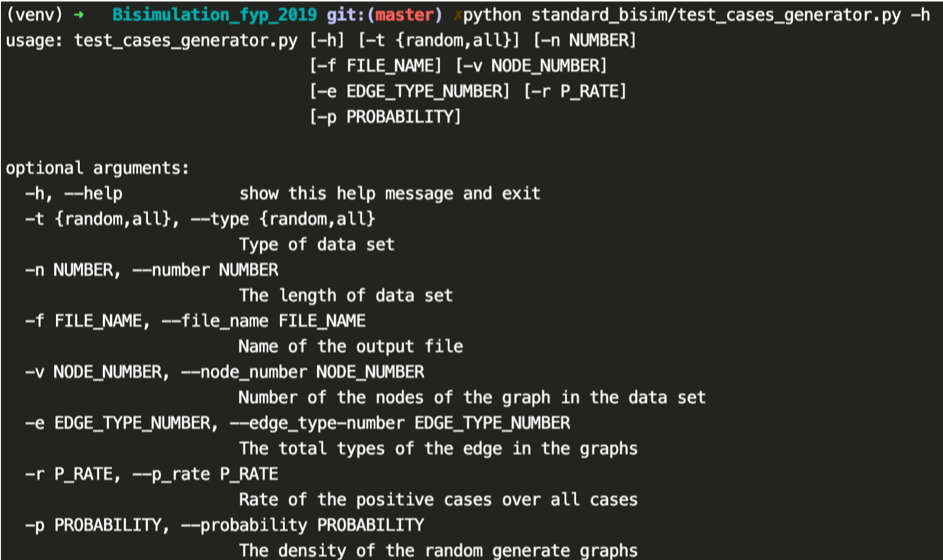
\includegraphics[width=0.9\textwidth]{img/generator.png}
    \caption{Arguments of test cases generator}
    \label{fig:arggenerator}
\end{figure}

% \captionof{listing}{Random test case generator \label{lst:ramgene}}\vspace{-0.6em}
\begin{code}
\caption{Random test case generator}
\label{lst:ramgene}
\begin{minted}[linenos, frame=single,breaklines]{python}
def test_cases_generator(c_type="random", number=100, file_name="test_cases", min_node_number=5, edge_type_number=3, probability=0.5, p_rate=0.5):
    labels = [chr(97 + i) for i in xrange(edge_type_number)]
    if not os.access('./data/', os.R_OK):
        os.mkdir('./data/')
    with open('./data/' + file_name + '.csv', 'w') as csvfile:
        print('write in path: ' + './data/' + file_name + '.csv')
        if c_type == 'random':
            fieldnames = ['g1', 'g2', 'bis']
            writer = csv.DictWriter(csvfile, fieldnames=fieldnames)
            writer.writeheader()

            for _ in xrange(number):
                if _ % (number/10) == 0: print("generating # %d" % _)
                g1 = ''
                while not g1 or not nx.is_weakly_connected(g1):
                    g1 = random_labeled_digraph(min_node_number, edge_type_number, random.random() * probability)
                g1_bin = get_bin_array_from_graph(g1, min_node_number, edge_type_number)
                bis = 1
                if random.random() > p_rate:
                    g2 = generate_random_similar(g1, edge_type_number)
                else:
                    g2 = random_labeled_digraph(min_node_number, edge_type_number, random.random() * probability)
                    k = bi.BisimPnT(labels, g1, g2)
                    bis = int(k.is_bisimilar())
                g2_bin = get_bin_array_from_graph(g2, min_node_number, edge_type_number)
                writer.writerow({fieldnames[0]: g1_bin, fieldnames[1]: g2_bin, fieldnames[2]: bis})
\end{minted}
\end{code}

% \captionof{listing}{Function of generating random bisimilar graph \label{lst:genrdmsim}}\vspace{-0.6em}
\begin{code}
\caption{Function of generating random bisimilar graph}
\label{lst:genrdmsim}
\begin{minted}[linenos, frame=single,breaklines]{python}
def generate_random_similar(graph, edge_type_number):
    k = bi.BisimPnT([chr(97 + t) for t in range(edge_type_number)], graph)
    min_graph = k.get_min_graph()
    min_node_number = min_graph.order()
    partition = [{i} for i in range(min_node_number)]
    node_number = graph.order()
    if min_node_number == node_number:
        return random_relabel_nodes(graph)
    for i in xrange(min_node_number, node_number):
        partition[random.randint(0, min_node_number - 1)].add(i)
    result_graph = None
    # print min_node_number, node_number
    while not result_graph or result_graph.order() != graph.order():
        result_graph = nx.MultiDiGraph()
        for start_node_type in xrange(min_node_number):
            for end_node_type in min_graph.successors(start_node_type):  # for each origin type pair
                for edge_label in {edge['label'] for edge in min_graph.get_edge_data(start_node_type, end_node_type).values()}:
                    # for each type edge
                    accept = False
                    while not accept:
                        start_nodes = random.sample(partition[start_node_type], random.randint(0, len(partition[start_node_type])))
                        for start_node in start_nodes:
                            end_nodes = random.sample(partition[end_node_type], random.randint(0, len(partition[end_node_type])))
                            for end_node in end_nodes:
                                exist_types = {exist_type_dic['label'] for exist_type_dic in result_graph.get_edge_data( start_node,end_node, default={0:{'label':'#'}}).values()}
                                if  edge_label not in exist_types:
                                    result_graph.add_edge(start_node, end_node, label=edge_label)
                        t1 = partition[start_node_type].copy()
                        t2 = partition[end_node_type].copy()
                        for start_node in partition[start_node_type]:
                            for end_node in partition[end_node_type]:
                                exist_types = {exist_type_dic['label'] for exist_type_dic in result_graph.get_edge_data( start_node,end_node, default={0:{'label':'#'}}).values()}
                                if edge_label in exist_types:
                                    t1.discard(start_node)
                                    t2.discard(end_node)
                        accept = not bool(t1) and not bool(t2)
    return result_graph
\end{minted}
\end{code}


\subsubsection{Implementation of Machine Learning}
This neural network is developed on the \texttt{Tensorflow} along with the visualisation tool \texttt{TensorBoard}.
TensorFlow Graph is a computation graph drew by \texttt{TensorBoard} that indicates the process of the computation.
Figure \ref{fig:tfgraph} are the TensorFlow graph of the network model .

After all parameters are randomly initialised by \texttt{tf.random\char`_normal\char`_initialiser()}, the model start with a fixed length ($mn^2$) input layer, and accept the numeral input, i.e. the 1 or 0 in the adjacency matrix are accepted as a number rather than a catalogue.
And the activate function used here is rectified linear unite (ReLU).
Because it is computationally efficient and more plausible on biology which may improve the comprehension of the model.
Also it promises fewer problems on vanishing gradient \cite{pmlr-v15-glorot11a}.
The adjacency matrixes become tensor after input.
Then the tensor of each graph goes through the re-representing part (see g1\_p and g2\_p in Figure \ref{fig:tfgraph}).
After that, they are merged into one big tensor and go through the distinguishing part (see merge and logits in Figure \ref{fig:tfgraph}).
At the end of the distinguishing part, the tensor is output as logits, i.e. two number that indicated the possibility of bisimilar or not.
Finally pass through a \emph{softmax} layer the prediction will be given.
Yet, during the training, there are metrics including loss, accuracy, precision, recall logged for further studying.
The main code is shown in Listing \ref{lst:mlat}.
It is also packed as a commend line tools (see Figure \ref{fig:argmlal}).

\begin{figure}[h]
\centering
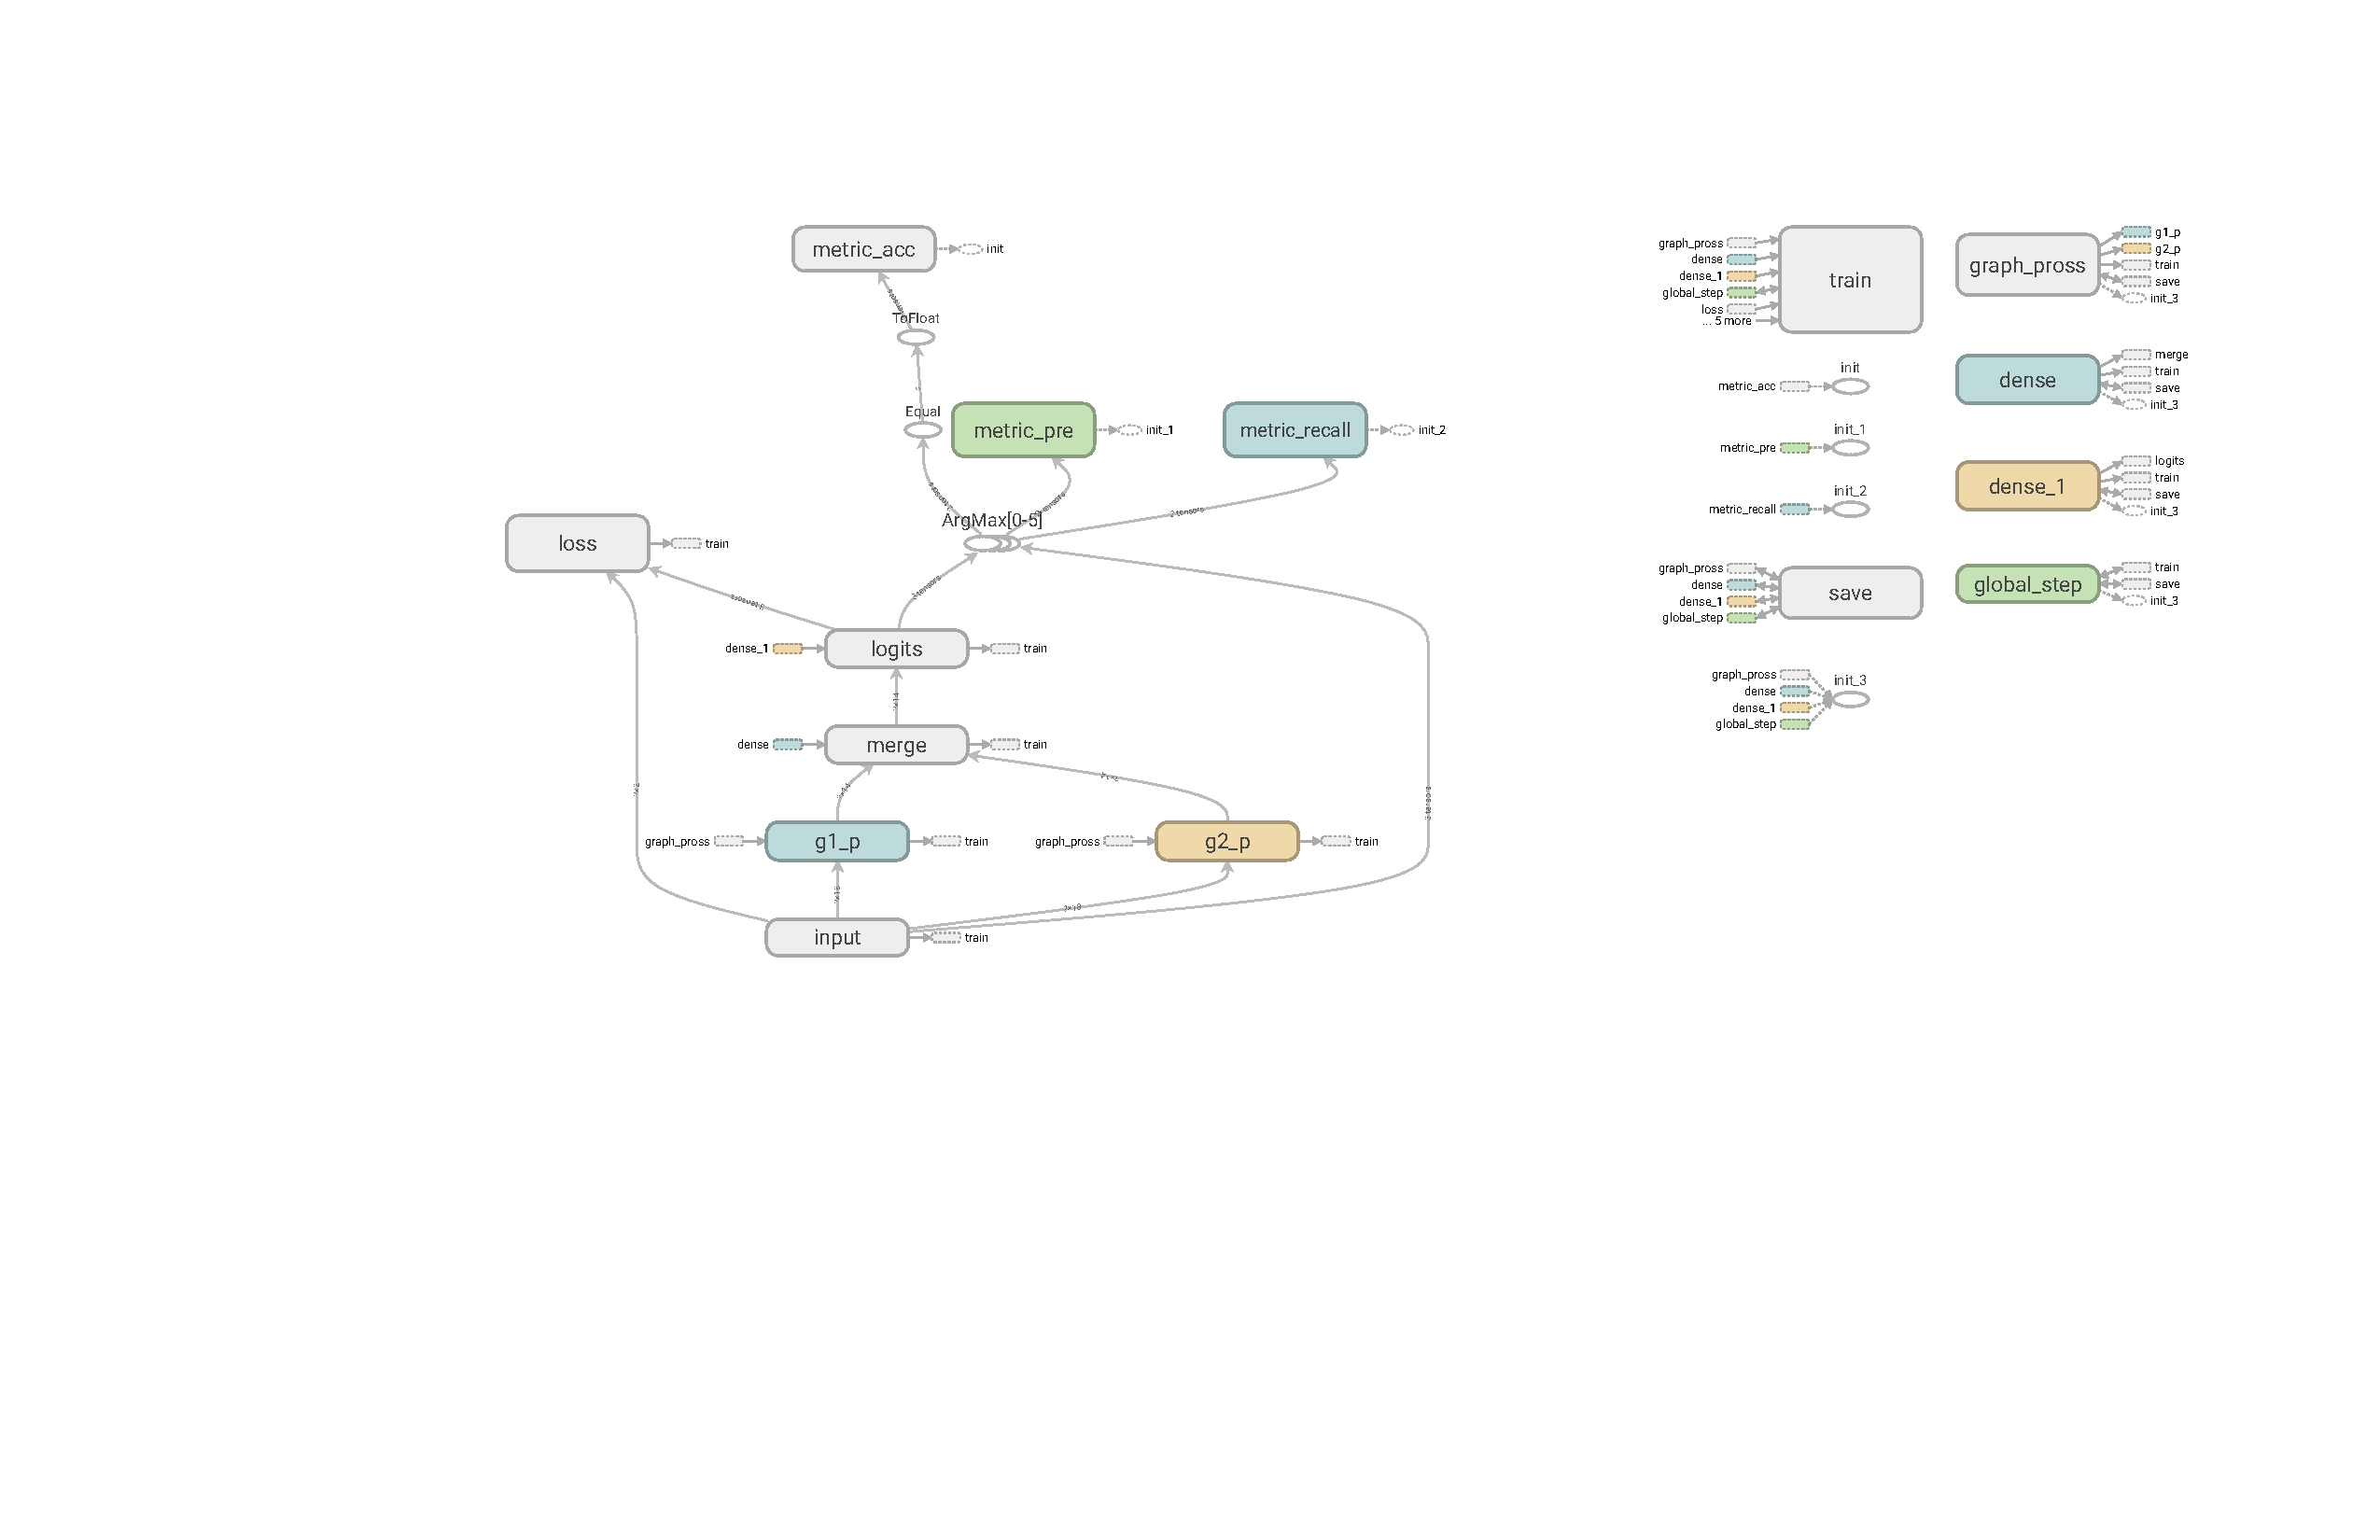
\includegraphics[width=\textwidth]{img/tfgraph.pdf}
\caption{TensorFlow graph of MLP}
\label{fig:tfgraph}
\end{figure}

\begin{figure}[h]
    \centering
    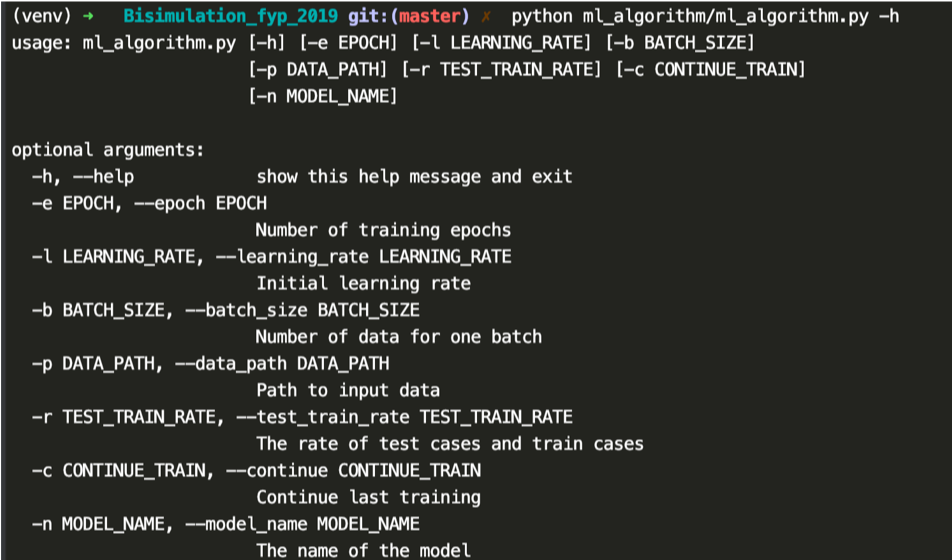
\includegraphics[width=0.9\textwidth]{img/mlalgorithm.png}
    \caption{Arguments of machine learning algorithm}
    \label{fig:argmlal}
\end{figure}


% \captionof{listing}{ML algorithm and training \label{lst:mlat}}\vspace{-0.6em}
\begin{code}
\caption{ML algorithm and training}
\label{lst:mlat}
\begin{minted}[linenos, frame=single,breaklines]{python}
def fc(self, continue_train=False):

    kernel_initializer = tf.initializers.glorot_normal()
    tf.reset_default_graph()
    small_layer_number = int(math.log(self.tupe_length) * 5)
    # print small_layer_number, self.tupe_length
    with tf.name_scope('input'):
        g1 = tf.placeholder(tf.float32, [None, self.tupe_length])
        g2 = tf.placeholder(tf.float32, [None, self.tupe_length])
        y = tf.placeholder(tf.float32, [None, 2])

    with tf.name_scope('g1_p'):
        with tf.variable_scope('graph_pross'):
            g1_dence1 = tf.layers.dense(g1, self.tupe_length, activation=tf.nn.relu, kernel_initializer=kernel_initializer, bias_initializer=tf.random_normal_initializer(), name='dence1')

            g1_s_dence1 = tf.layers.dense(g1_dence1, small_layer_number, activation=tf.nn.relu, kernel_initializer=kernel_initializer, bias_initializer=tf.random_normal_initializer(), name='s_dence1')

    with tf.name_scope('g2_p'):
        with tf.variable_scope('graph_pross', reuse=True):
            g2_dence1 = tf.layers.dense(g2, self.tupe_length, activation=tf.nn.relu, name='dence1', reuse=True)

            g2_s_dence1 = tf.layers.dense(g2_dence1, small_layer_number, activation=tf.nn.relu, name='s_dence1', reuse=True)
    with tf.name_scope('merge'):
        two_graphs = tf.concat([g1_s_dence1, g2_s_dence1], 1)
        merge_layer = tf.layers.dense(two_graphs, small_layer_number, activation=tf.nn.relu, kernel_initializer=kernel_initializer, bias_initializer=tf.random_normal_initializer())
    with tf.name_scope('logits'):
        logits = tf.layers.dense(merge_layer, 2, activation=tf.identity, kernel_initializer=kernel_initializer, bias_initializer=tf.random_normal_initializer())
    with tf.name_scope('loss'):
        loss = tf.losses.softmax_cross_entropy(y, logits)
        tf.summary.scalar('loss', loss)

    global_step = tf.Variable(0, trainable=False, name='global_step')

    with tf.name_scope('train'):
        train = tf.train.AdadeltaOptimizer(learning_rate=self.learning_rate) .minimize(loss=loss, global_step=global_step)

    acc_metric, acc_metric_update = tf.metrics.accuracy(tf.argmax(logits, 1), tf.argmax(y, 1), name='metric_acc')
    pre_metric, pre_metric_update = tf.metrics.precision(tf.argmax(logits, 1), tf.argmax(y, 1), name='metric_pre')
    recall_metric, recall_metric_update = tf.metrics.recall(tf.argmax(logits, 1), tf.argmax(y, 1), name='metric_recall')
    tf.summary.scalar('accuracy', acc_metric_update)
    tf.summary.scalar('precision', pre_metric_update)
    tf.summary.scalar('recall', recall_metric_update)

    metric_acc_var = tf.get_collection(tf.GraphKeys.LOCAL_VARIABLES, scope="metric_acc")
    acc_initializer = tf.variables_initializer(var_list=metric_acc_var)
    metric_pre_var = tf.get_collection(tf.GraphKeys.LOCAL_VARIABLES, scope="metric_pre")
    pre_initializer = tf.variables_initializer(var_list=metric_pre_var)
    metric_recall_var = tf.get_collection(tf.GraphKeys.LOCAL_VARIABLES, scope="metric_recall")
    recall_initializer = tf.variables_initializer(var_list=metric_recall_var)

    merged_summary = tf.summary.merge_all()
    saver = tf.train.Saver()

    with tf.Session() as sess:
        if continue_train:
            saver.restore(sess, DIR_MODEL + '/' + self.model_name + '/model.ckpt')
            print('continue training, model loaded')
        else:
            self.clean_old_record()
            print('new training, old record cleaned')
            # initial
            sess.run(tf.global_variables_initializer())

        train_writer = tf.summary.FileWriter(DIR_SUMMARY + '/' + self.model_name, sess.graph)
        test_writer = tf.summary.FileWriter(DIR_SUMMARY + '/' + self.model_name + '_test')

        for epoch in range(self.epochs):
            sess.run([acc_initializer, pre_initializer, recall_initializer])
            loss_p = None
            g_step = None

            summary_11, g_step_1= sess.run([merged_summary,global_step], feed_dict={g1: self.g1_dfs[1], g2: self.g2_dfs[1], y: self.label_dfs[1]})

            test_writer.add_summary(summary_11, g_step_1)

            for i in range(self.batch_number):
                _, loss_p, summary, g_step = sess.run([train, loss, merged_summary, global_step], feed_dict={g1: self.g1_dfs[0][i], g2: self.g2_dfs[0][i], y: self.label_dfs[0][i]})
                train_writer.add_summary(summary, g_step)

            if epoch % 10 == 0:
                # summary,acc = sess.run([merged_summary ,acc_metric])
                acc, pre, recall = sess.run([acc_metric, pre_metric, recall_metric])
                log_str = "Epoch %d \t G_step %d \t Loss=%f \t Accuracy=%f \t Precision=%f \t Recall=%f "
                print(log_str % (epoch, g_step, loss_p, acc, pre, recall))
                saver.save(sess, DIR_MODEL + '/' + self.model_name + '/model.ckpt')

    train_writer.close()
    test_writer.close()
\end{minted}
\end{code}


\newpage
\subsection{Components Test}
\label{sec:comptest}
During the development, some tests are used for examining each component.
Here some of the test cases and the test results will be given.

\subsubsection{Test for Standard Bisimulation Algorithm}
The test cases used here is from the textbook.
And by manipulating these cases, this component can be tested.

\vspace{+0.2em}
\noindent\textbf{Test case 1:}

\noindent This case is form \cite{Stirling2011a}. 
By changing two egdes in this case (i.e. $\text{H-4}\stackrel{b}{\rightarrow}\text{H-5} \Longrightarrow \text{H-4}\stackrel{c}{\rightarrow}\text{H-5}$, $\text{G-2}\stackrel{b}{\rightarrow}\text{G-4} \Longrightarrow \text{G-2}\stackrel{c}{\rightarrow}\text{G-4}$), these two graph should lose bisimulation equivalence.
The test code is shown in Listing \ref{lst:test1}.
The output is shown in Figure \ref{fig:output1}-\ref{fig:output1g-}.
Notice that in a figure like Figure \ref{fig:output1g}, edges that are one type has the same colour and nodes in the same partition (i.e. are bisimilar) will be painted in the same colour.
% \captionof{listing}{Test code for case 1 \label{lst:test1}}
% \vspace{-0.5em}
\begin{code}
\caption{Test code for case 1}
\label{lst:test1}
\begin{minted}[linenos, frame=single,breaklines]{python}
# =============== example 1 ===============
G = nx.MultiDiGraph()
G.add_edge(5, 2, label='a')
G.add_edge(2, 3, label='b')
G.add_edge(2, 4, label='b')
# G.add_edge(2, 4, label='c')

H = nx.MultiDiGraph()
H.add_edge(1, 2, label='a')
H.add_edge(1, 4, label='a')
H.add_edge(2, 3, label='b')
H.add_edge(4, 5, label='b')
# H.add_edge(4, 5, label='c')

labels = ['a', 'b']
# labels = ['a', 'b', 'c']

k = BisimPnT(labels, G, H)
par = k.coarsest_partition()
vi.plot_graph_with_partition(k.full_graph_U,par,'example_1')
vi.plot_graph(BisimPnT(labels,H).get_min_graph(), 'mini_g')
print("Example 1: ")
print(par)
print(k.is_bisimilar())
\end{minted}
\end{code}

\begin{figure}[H]
\centering
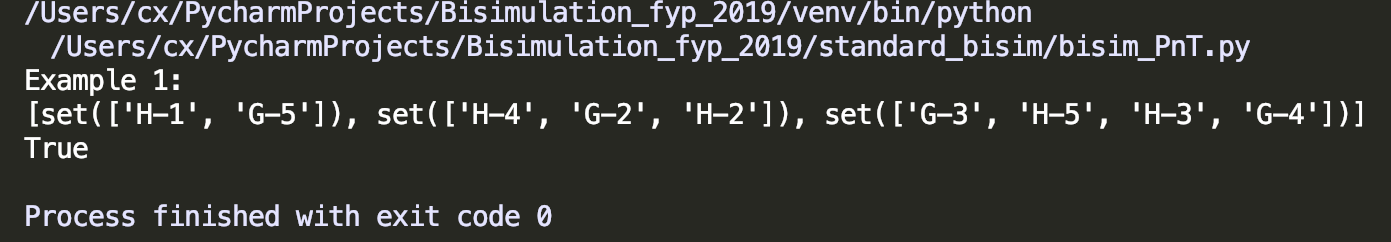
\includegraphics[width=0.9\textwidth]{img/output1.png}
\caption{Output for test case 1 positive instance}
\label{fig:output1}
\end{figure}

\begin{figure}[H]
    \centering
    \subfigure[Mini graph]{
        % \label{fig:example1_model}
        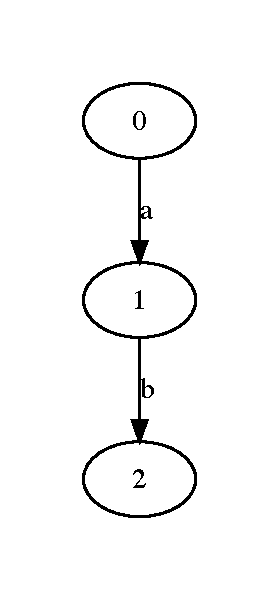
\includegraphics[height=16em]{img/output1min.pdf}}
    \subfigure[Coloured graphs]{
        % \label{fig:example1_matrix}
        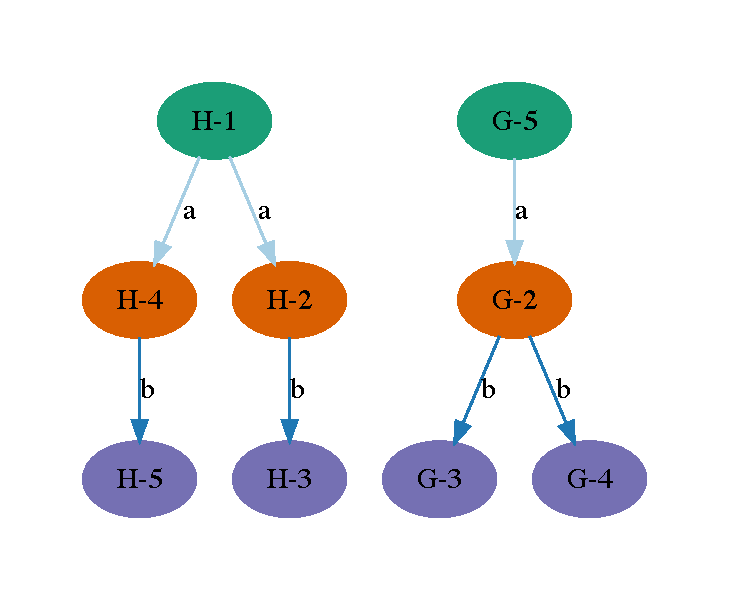
\includegraphics[height=16em]{img/output1g.pdf}}
    \caption{Test case 1: positive instance}
    \label{fig:output1g}
\end{figure}

\begin{figure}[H]
\centering
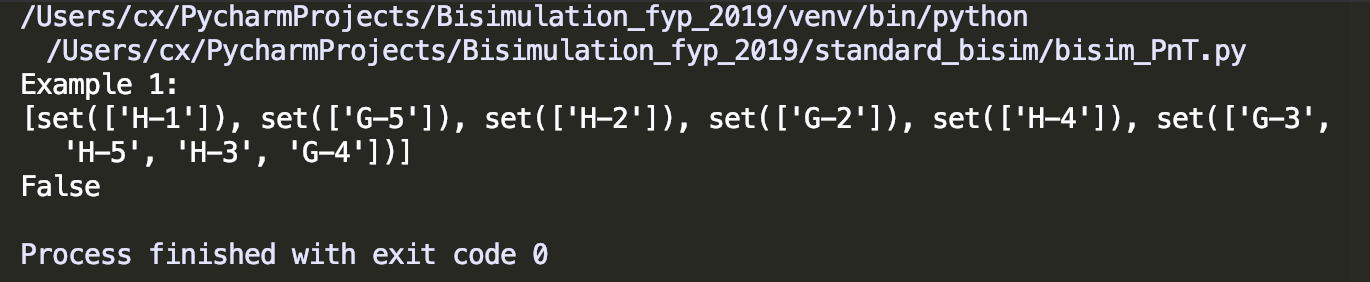
\includegraphics[width=0.9\textwidth]{img/output1-.png}
\caption{Output for test case 1 negative instance}
\label{fig:output1-}
\end{figure}

\begin{figure}[H]
    \centering
    % \label{fig:example1_matrix}
    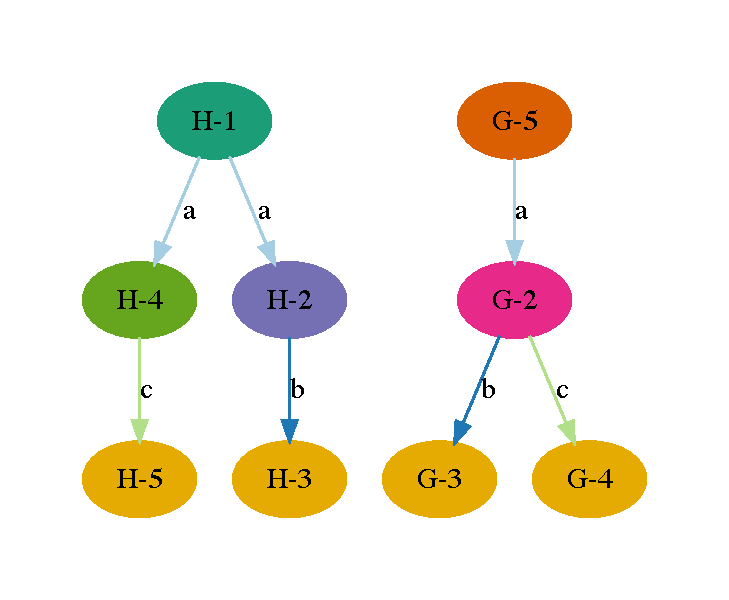
\includegraphics[height=16em]{img/output1g-.pdf}
    \caption{Test case 1: negative instance}
    \label{fig:output1g-}
\end{figure}

\vspace{+0.2em}
\noindent\textbf{Test case 2:}

\noindent This case is form \cite{Stirling2011a}.
By changing two egdes in this case (i.e. $\text{G-3}\stackrel{c}{\rightarrow}\text{G-2} \Longrightarrow \text{G-3}\stackrel{b}{\rightarrow}\text{G-2}$ these two graph should lose bisimulation equivalence.
The test code is shown in Listing \ref{lst:test2}.
The output of the test result is shown in Figure \ref{fig:output2}-\ref{fig:output2g-}.
% \captionof{listing}{Test code for case 2 \label{lst:test2}}\vspace{-0.5em}
\begin{code}
\caption{Test code for case 2}
\label{lst:test2}
\begin{minted}[linenos, frame=single,breaklines]{python}
# =============== example 2 ===============
G = nx.MultiDiGraph()
G.add_edge(1, 3, label='a')
G.add_edge(1, 2, label='a')
G.add_edge(2, 3, label='b')
G.add_edge(3, 1, label='c')
G.add_edge(3, 2, label='c')
# G.add_edge(3, 2, label='b')

H = nx.MultiDiGraph()
H.add_edge(1, 3, label='a')
H.add_edge(1, 4, label='a')
H.add_edge(2, 3, label='b')
H.add_edge(3, 1, label='c')
H.add_edge(3, 4, label='c')
H.add_edge(4, 5, label='b')
H.add_edge(5, 1, label='c')
H.add_edge(5, 2, label='c')

labels = ['a', 'b', 'c']
k = BisimPnT(labels, G, H)
partition = k.coarsest_partition()
vi.plot_graph_with_partition(k.full_graph_U, partition, 'example_2')
vi.plot_graph(BisimPnT(labels, H).get_min_graph(), 'mini_g2')
print("Example 2: ")
print(partition)
print(k.is_bisimilar())
\end{minted}
\end{code}

\begin{figure}[H]
\centering
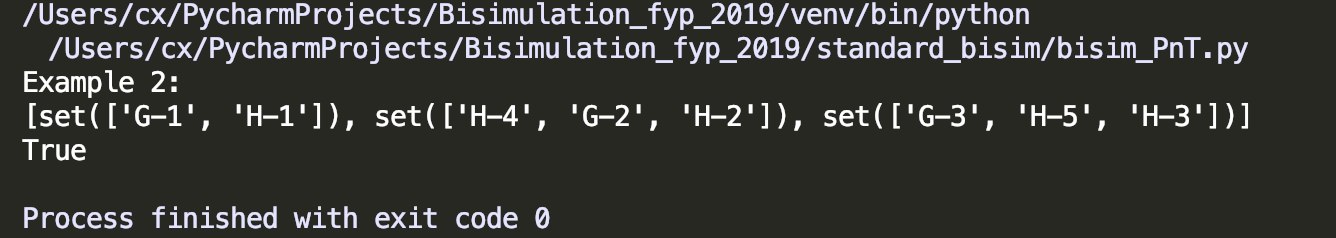
\includegraphics[width=0.9\textwidth]{img/output2.png}
\caption{Output for test case 2 positive instance}
\label{fig:output2}
\end{figure}

\begin{figure}[H]
    \centering
    \subfigure[Mini graph]{
        % \label{fig:example1_model}
        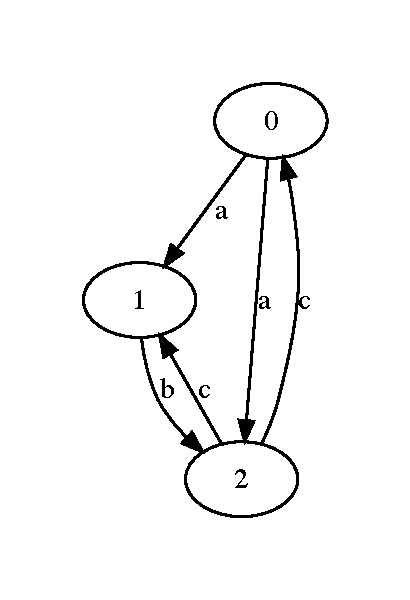
\includegraphics[height=14em]{img/output2min.pdf}}
    \subfigure[Coloured graphs]{
        % \label{fig:example1_matrix}
        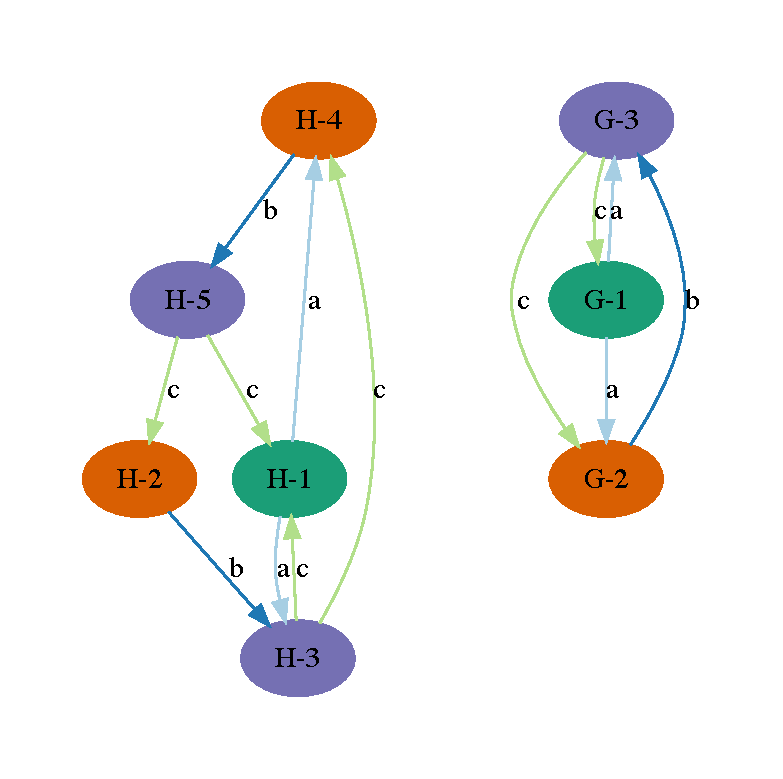
\includegraphics[height=16em]{img/output2g.pdf}}
    \caption{Test case 2: positive instance}
    \label{fig:output2g}
\end{figure}

\begin{figure}[H]
\centering
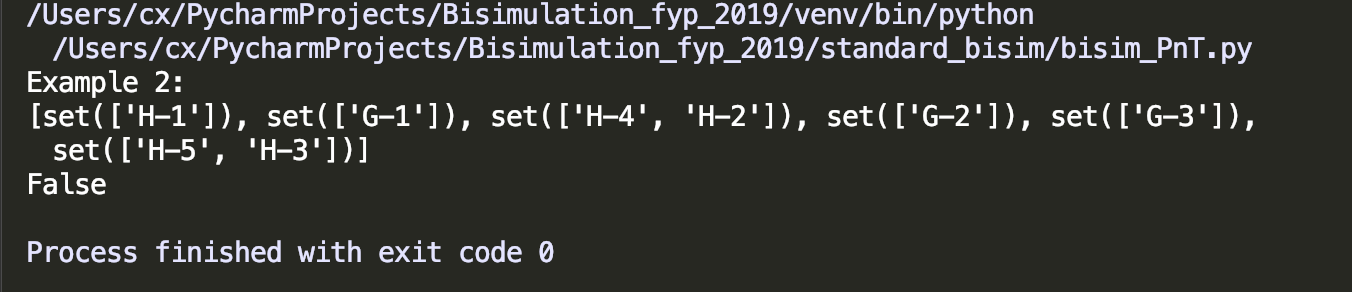
\includegraphics[width=0.9\textwidth]{img/output2-.png}
\caption{Output for test case 1 negative instance}
\label{fig:output2-}
\end{figure}
\begin{figure}[H]
    \centering
    % \label{fig:example1_matrix}
    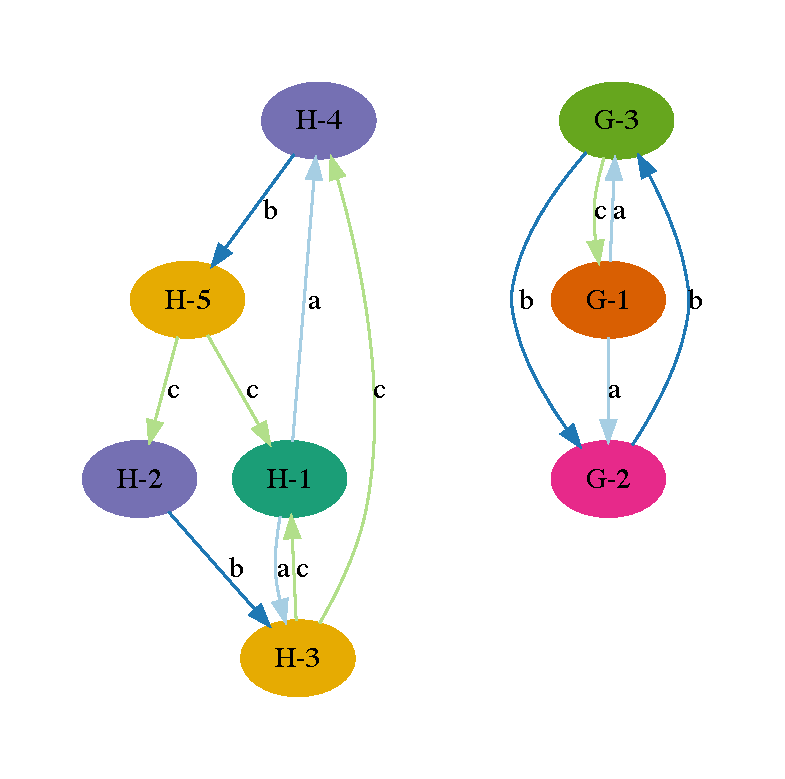
\includegraphics[height=16em]{img/output2g-.pdf}
    \caption{Test case 2: negative instance}
    \label{fig:output2g-}
\end{figure}

\subsubsection{Test for test case generator}

\textbf{Function for Generating Random bisimilar Graph:}

\noindent Firstly the function \texttt{generate\char`_random\char`_similar()} is tested.
The idea of testing is to randomly generate a graph then call the function.
Use the \emph{standard bisimulation algorithm} to compute the bisimulation equivalence of the output (to be seen in Listing \ref{lst:testg}).
Here, we also give some test generated results (see Figure \ref{fig:outputg1}-\ref{fig:outputg4}).
Notice that these results are selected examples for different types of result.


% \captionof{listing}{Test code for \texttt{generate\char`_random\char`_similar} \label{lst:testg}}\vspace{-0.5em}
\begin{code}
\caption{Test code for \texttt{generate\char`_random\char`_similar}}
\label{lst:testg}
\begin{minted}[linenos, frame=single,breaklines]{python}
# =============== test for random_labeled_digraph() ===============
flag = True
i = 0

# if there are any error the loop will break
# until reach the test time
while flag :
    i = i+1
    a = random_labeled_digraph(5,2,0.5*random.random())
    b = generate_random_similar(a, 2)
    k = bi.BisimPnT(['a','b'],a,b)
    flag = k.is_bisimilar()
    print i
    print flag
    if i == 100:
        break

vi.plot_graph(a, 'test')
vi.plot_graph(bi.BisimPnT(['a','b'],a).get_min_graph(),"mini_a")
vi.plot_graph(b, 'test1')
vi.plot_graph(bi.BisimPnT(['a','b'],a).get_min_graph(),"mini_b")
\end{minted}
\end{code}


\begin{figure}[H]
    \centering
    \subfigure[Mini graph]{
        % \label{fig:example1_model}
        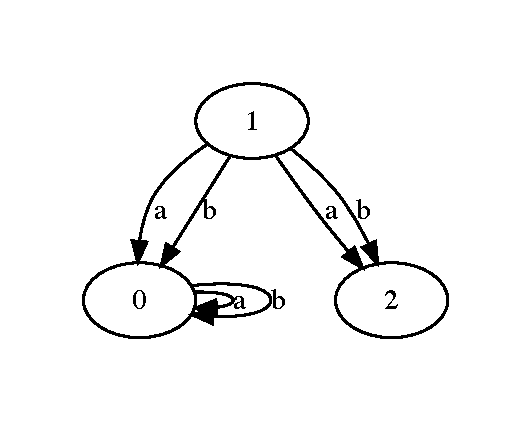
\includegraphics[height=9em]{img/outputg1m.pdf}}
    \subfigure[Coloured graphs]{
        % \label{fig:example1_matrix}
        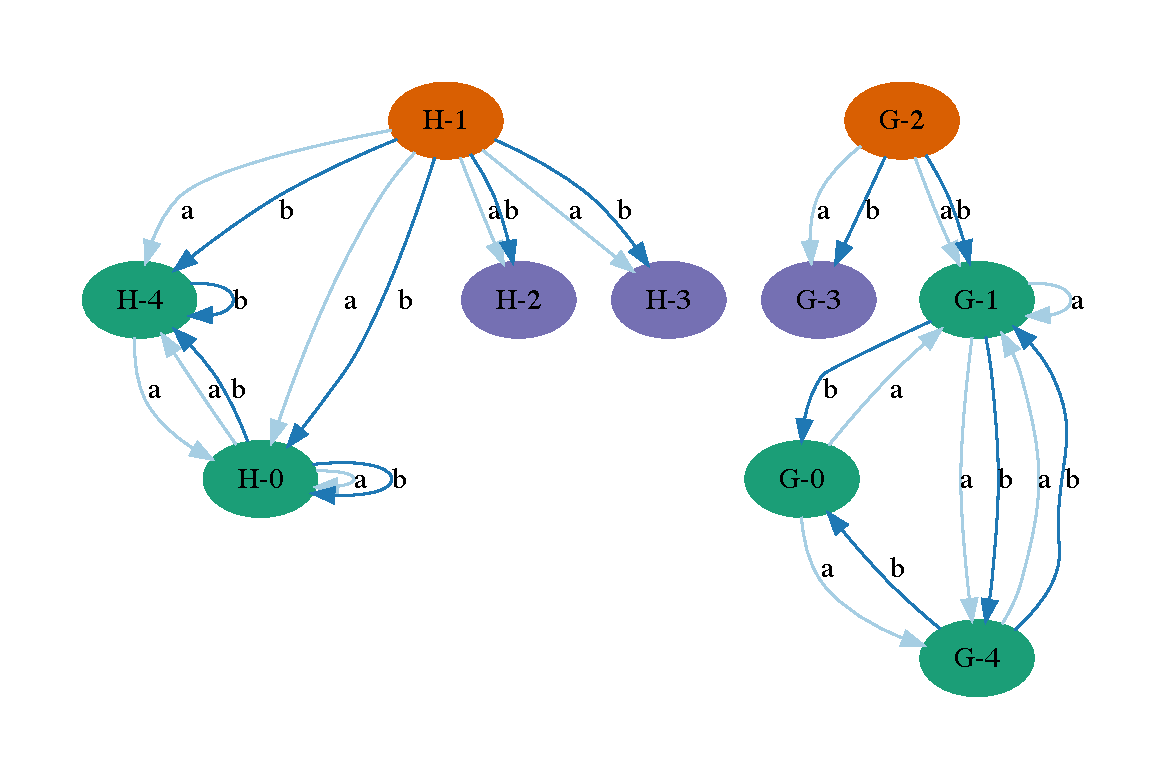
\includegraphics[height=17em]{img/outputg1.pdf}}
    \caption{Test result 1}
    \label{fig:outputg1}
\end{figure}

\begin{figure}[H]
    \centering
    \subfigure[Mini graph]{
        % \label{fig:example1_model}
        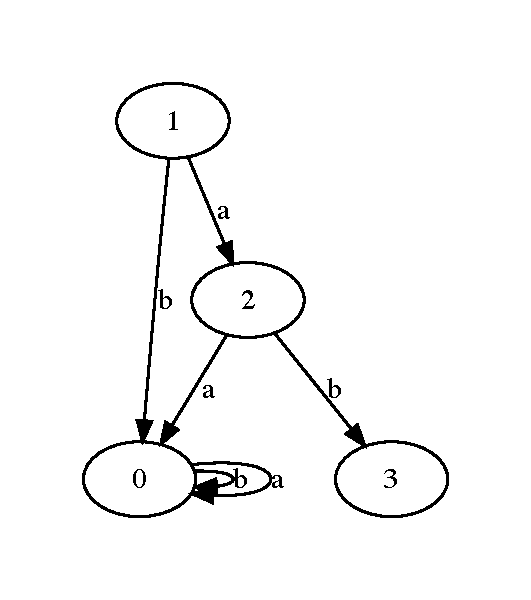
\includegraphics[height=12em]{img/outputg2m.pdf}}
    \subfigure[Coloured graphs]{
        % \label{fig:example1_matrix}
        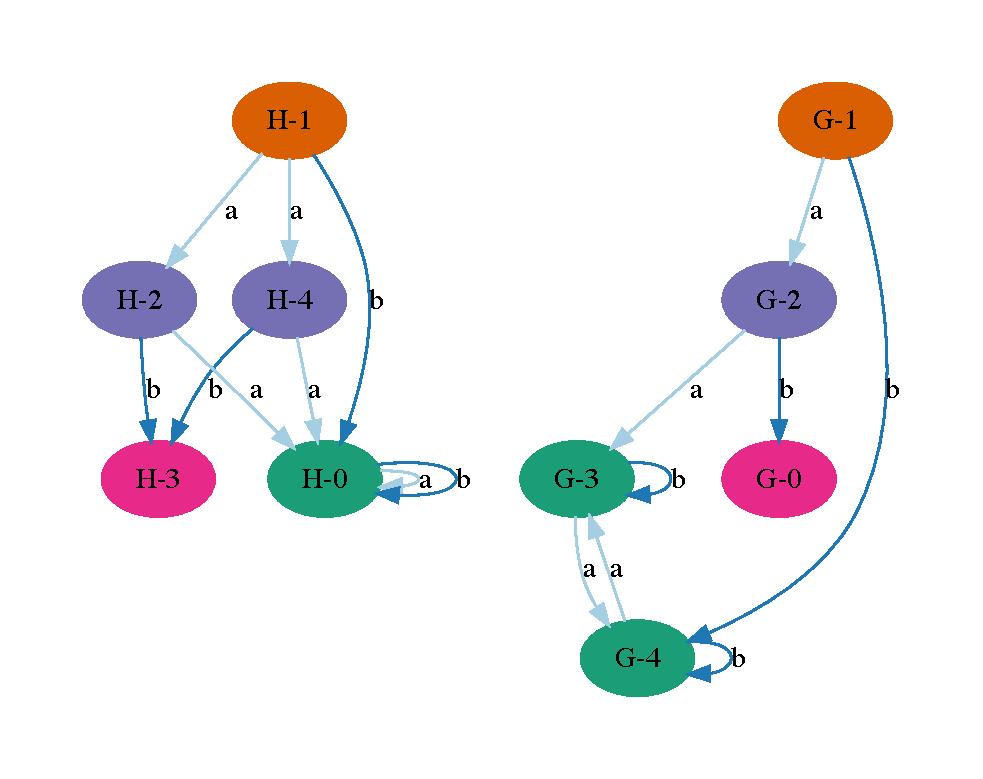
\includegraphics[height=17em]{img/outputg2.pdf}}
    \caption{Test result 2}
    \label{fig:outputg2}
\end{figure}

\begin{figure}[H]
    \centering
    \subfigure[Mini graph]{
        % \label{fig:example1_model}
        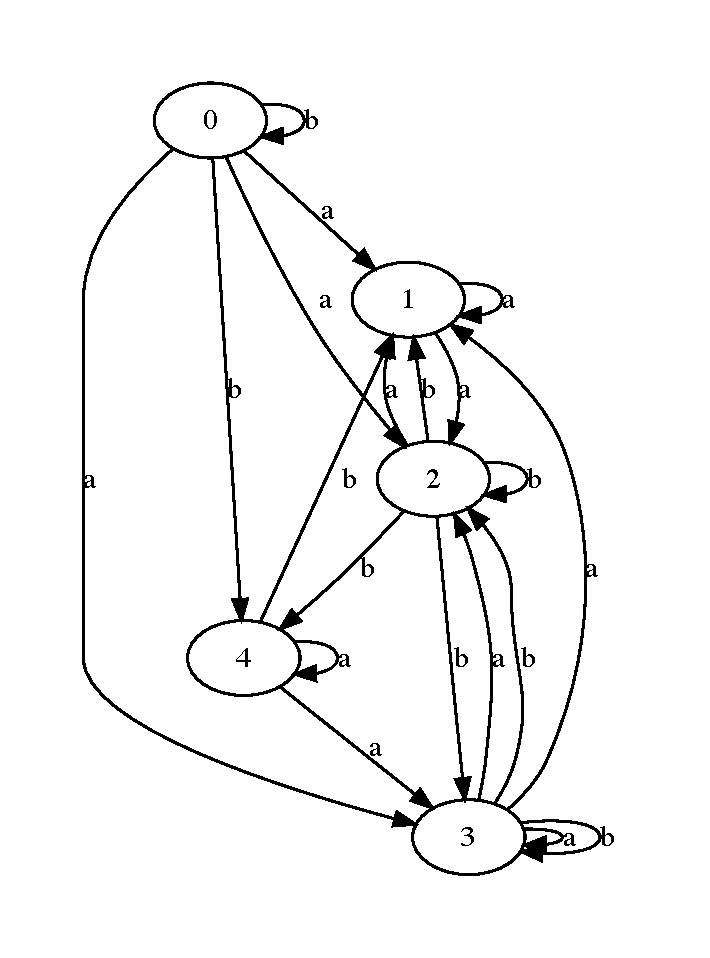
\includegraphics[height=15em]{img/outputg3m.pdf}}
    \subfigure[Coloured graphs]{
        % \label{fig:example1_matrix}
        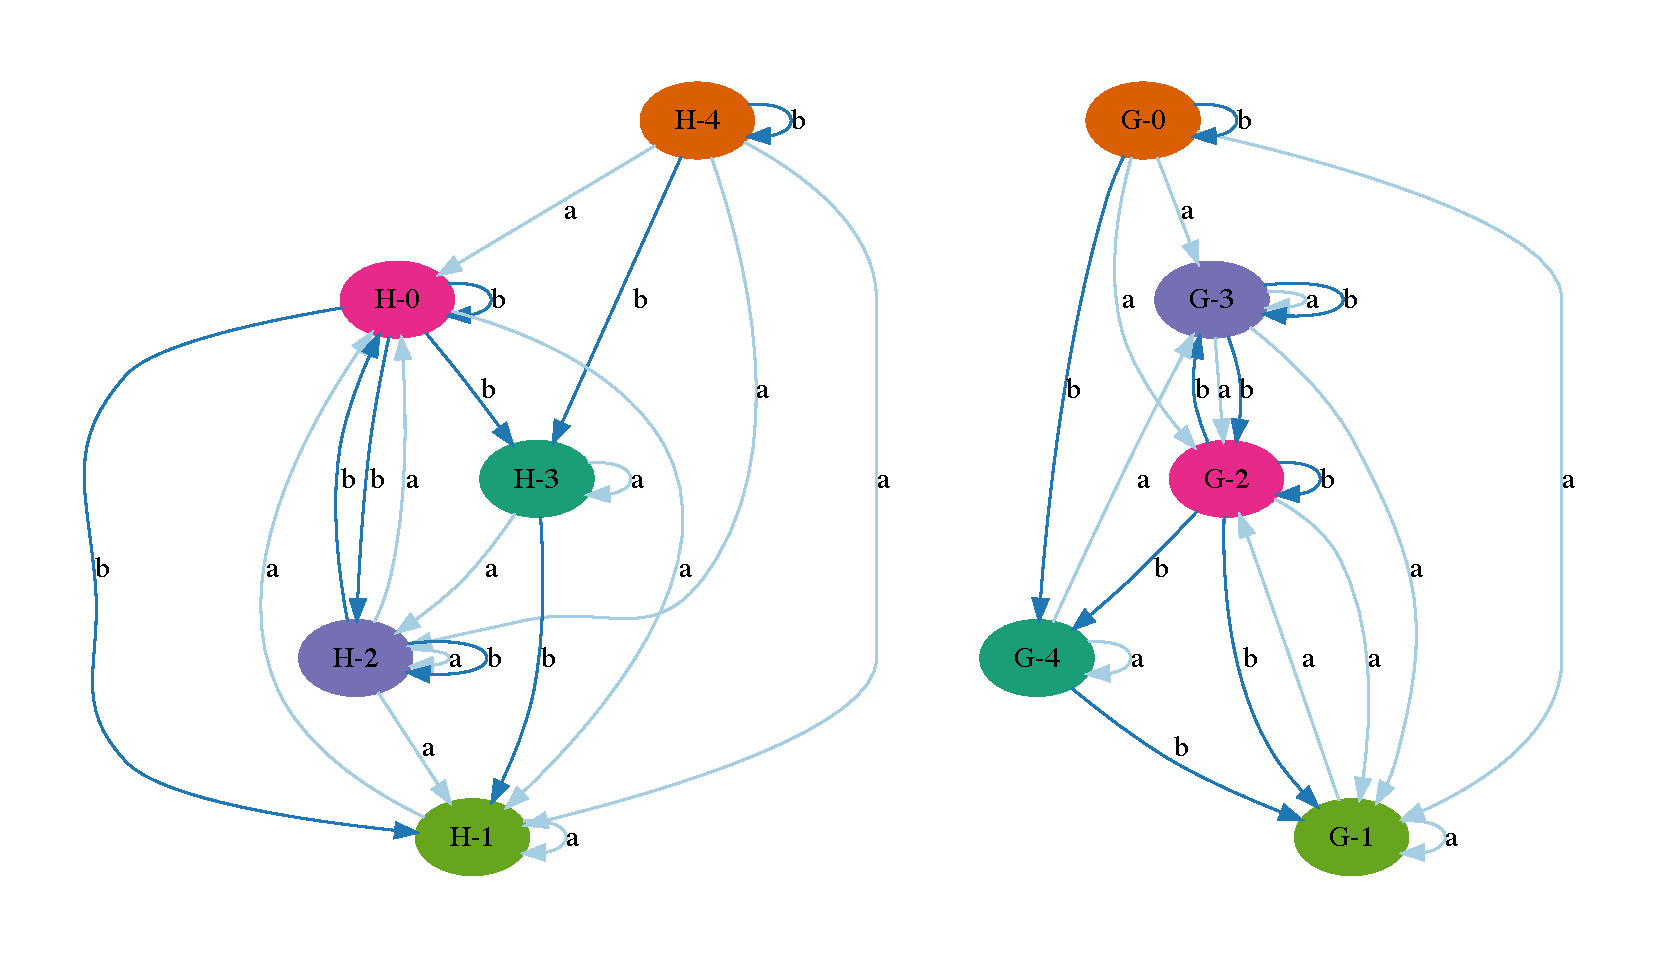
\includegraphics[height=15em]{img/outputg3.pdf}}
    \caption{Test result 3}
    \label{fig:outputg3}
\end{figure}

\begin{figure}[H]
    \centering
    \subfigure[Mini graph]{
        % \label{fig:example1_model}
        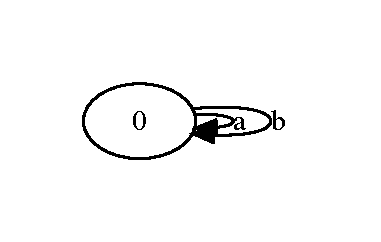
\includegraphics[height=4em]{img/outputg4m.pdf}}
    \subfigure[Coloured graphs]{
        % \label{fig:example1_matrix}
        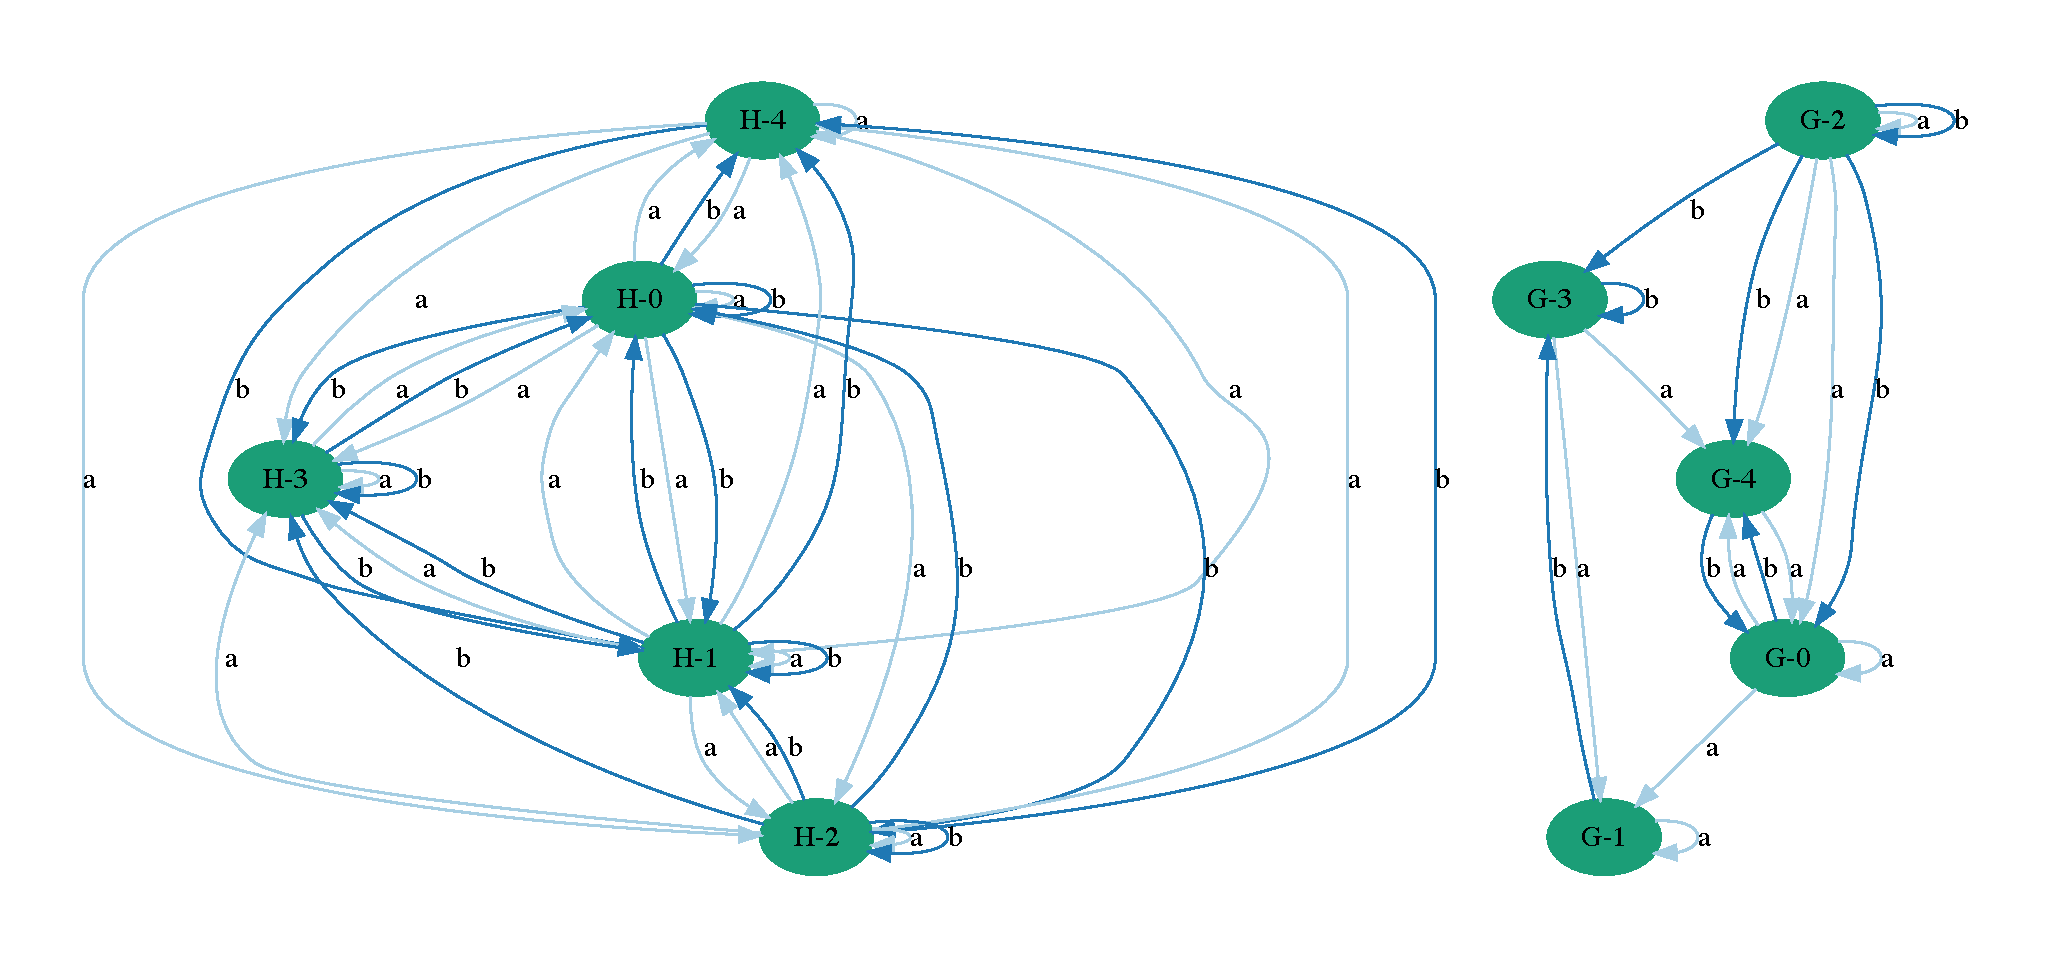
\includegraphics[height=14.5em]{img/outputg4.pdf}}
    \caption{Test result 4}
    \label{fig:outputg4}
\end{figure}


\noindent\textbf{Functions for generator:}
\noindent For the Generator, the test is for the I/O.
Here part of the file generated with 3 nodes and 2 types of edge is given in Table \ref{tab:partoffile}. 
And the running time screenshot is shown in Figure \ref{fig:runscreengen}.

\begin{figure}[h]
\centering
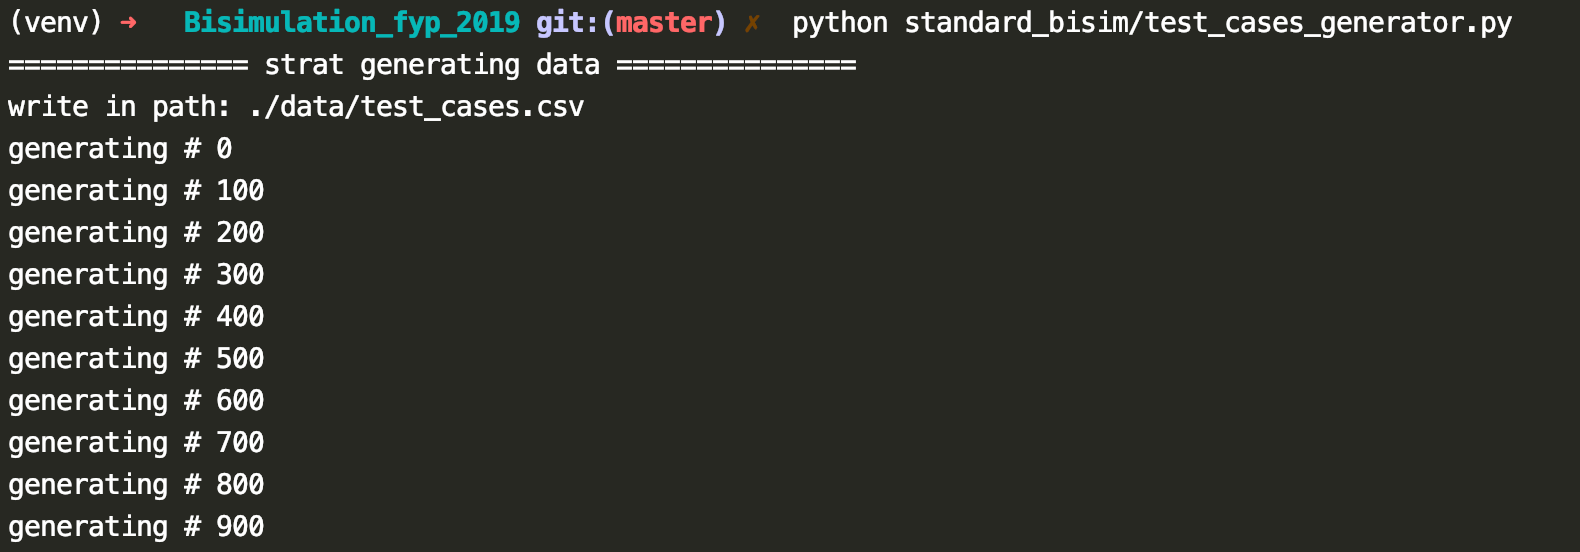
\includegraphics[width=\textwidth]{img/runscreengen.png}
\caption{Screen shot of generator running}
\label{fig:runscreengen}
\end{figure}

\begin{table}[h]
\small
\centering
\begin{tabular}{ |c|c|c| } 
 \hline
    g1 & g2 & bis \\
 \hline
    1, 1, 1, 1, 0, 1, 1, 0, 0, 0, 1, 1, 0, 1, 1, 1, 0, 1  &  0, 0, 0, 0, 0, 0, 1, 1, 0, 1, 0, 1, 1, 0, 0, 1, 1, 0  &  0 \\
    0, 1, 0, 0, 0, 0, 0, 1, 0, 1, 0, 0, 1, 0, 1, 0, 0, 0  &  0, 0, 1, 0, 1, 0, 0, 0, 0, 1, 0, 1, 0, 0, 0, 1, 0, 1  &  1 \\
    1, 0, 0, 1, 0, 0, 0, 0, 0, 1, 0, 0, 0, 1, 1, 0, 1, 0  &  0, 1, 0, 0, 0, 0, 0, 1, 1, 0, 0, 0, 1, 0, 0, 1, 1, 0  &  1 \\
    0, 0, 0, 0, 0, 1, 0, 0, 0, 0, 0, 1, 0, 0, 1, 0, 0, 0  &  1, 1, 1, 0, 1, 1, 0, 0, 0, 1, 0, 1, 1, 1, 0, 0, 0, 0  &  0 \\
    1, 0, 0, 1, 0, 0, 0, 0, 0, 0, 0, 0, 1, 1, 1, 0, 1, 1  &  0, 0, 1, 1, 0, 0, 0, 1, 1, 1, 1, 0, 1, 1, 1, 0, 1, 1  &  0 \\
    1, 0, 0, 0, 0, 0, 1, 0, 0, 0, 0, 0, 0, 0, 0, 1, 0, 0  &  0, 0, 1, 0, 0, 1, 0, 0, 0, 0, 0, 0, 0, 0, 0, 0, 0, 1  &  0 \\
    1, 0, 0, 0, 1, 1, 1, 1, 0, 0, 0, 0, 0, 1, 0, 0, 0, 0  &  0, 1, 0, 1, 1, 1, 1, 1, 1, 1, 1, 1, 0, 0, 1, 1, 0, 1  &  0 \\
    1, 1, 1, 1, 0, 0, 1, 0, 0, 0, 1, 0, 0, 1, 0, 1, 1, 0  &  1, 0, 0, 1, 0, 1, 0, 0, 1, 1, 1, 1, 1, 0, 1, 0, 0, 0  &  1 \\
    0, 1, 0, 1, 0, 0, 1, 0, 1, 1, 0, 0, 1, 1, 0, 0, 1, 1  &  0, 0, 0, 1, 0, 1, 1, 1, 1, 0, 1, 1, 1, 0, 1, 0, 0, 0  &  0 \\
    1, 1, 1, 0, 1, 0, 1, 1, 1, 1, 1, 1, 0, 1, 1, 0, 0, 1  &  1, 1, 1, 0, 1, 0, 1, 1, 1, 0, 1, 1, 1, 1, 1, 1, 1, 1  &  1 \\
    ...  & ...  & ... \\
 \hline
\end{tabular}
\caption{Part of the generated file \texttt{test\char`_cases.csv}}
\label{tab:partoffile}
\end{table}



\subsubsection{Test for ML Algorithm}
Here we will use some simple generated test cases.
And through the change of the metrics, the algorithm can be tested on some level.
Here give graphs of first 1000 epochs training of the test sample where the node number is 3 and the type number of edges is 2 and 1000 entries (see Figure \ref{fig:mlt1}), along with the running time screenshot (see Figure \ref{fig:runscreenml}).
The orange and blue lines indicate the trend of metrics on train data and test data respectively.
In Figure \ref{fig:mlt1acc}, along with the training the accuracy on training data and test data growth distinctively.
And in Figure \ref{fig:mlt1loss}, the loss on both data sets decreases.
Several tests show similar results.
It denotes that the model is actually learning as expected.

\begin{figure}[h]
\centering
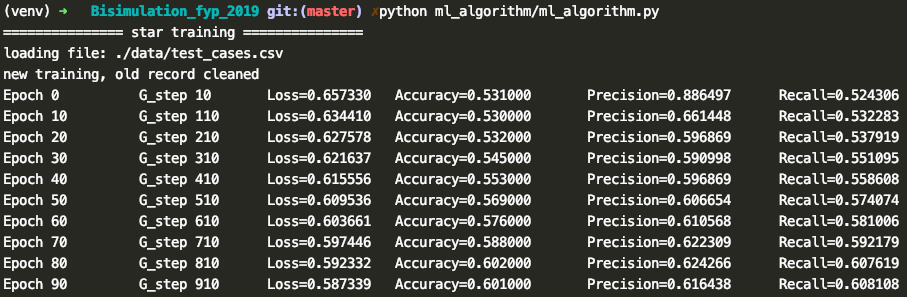
\includegraphics[width=\textwidth]{img/runscreenml.png}
\caption{Screen shot of machine learning algorithm running}
\label{fig:runscreenml}
\end{figure}

\begin{figure}[h]
    \centering
    \subfigure[Accuracy]{
        \label{fig:mlt1acc}
        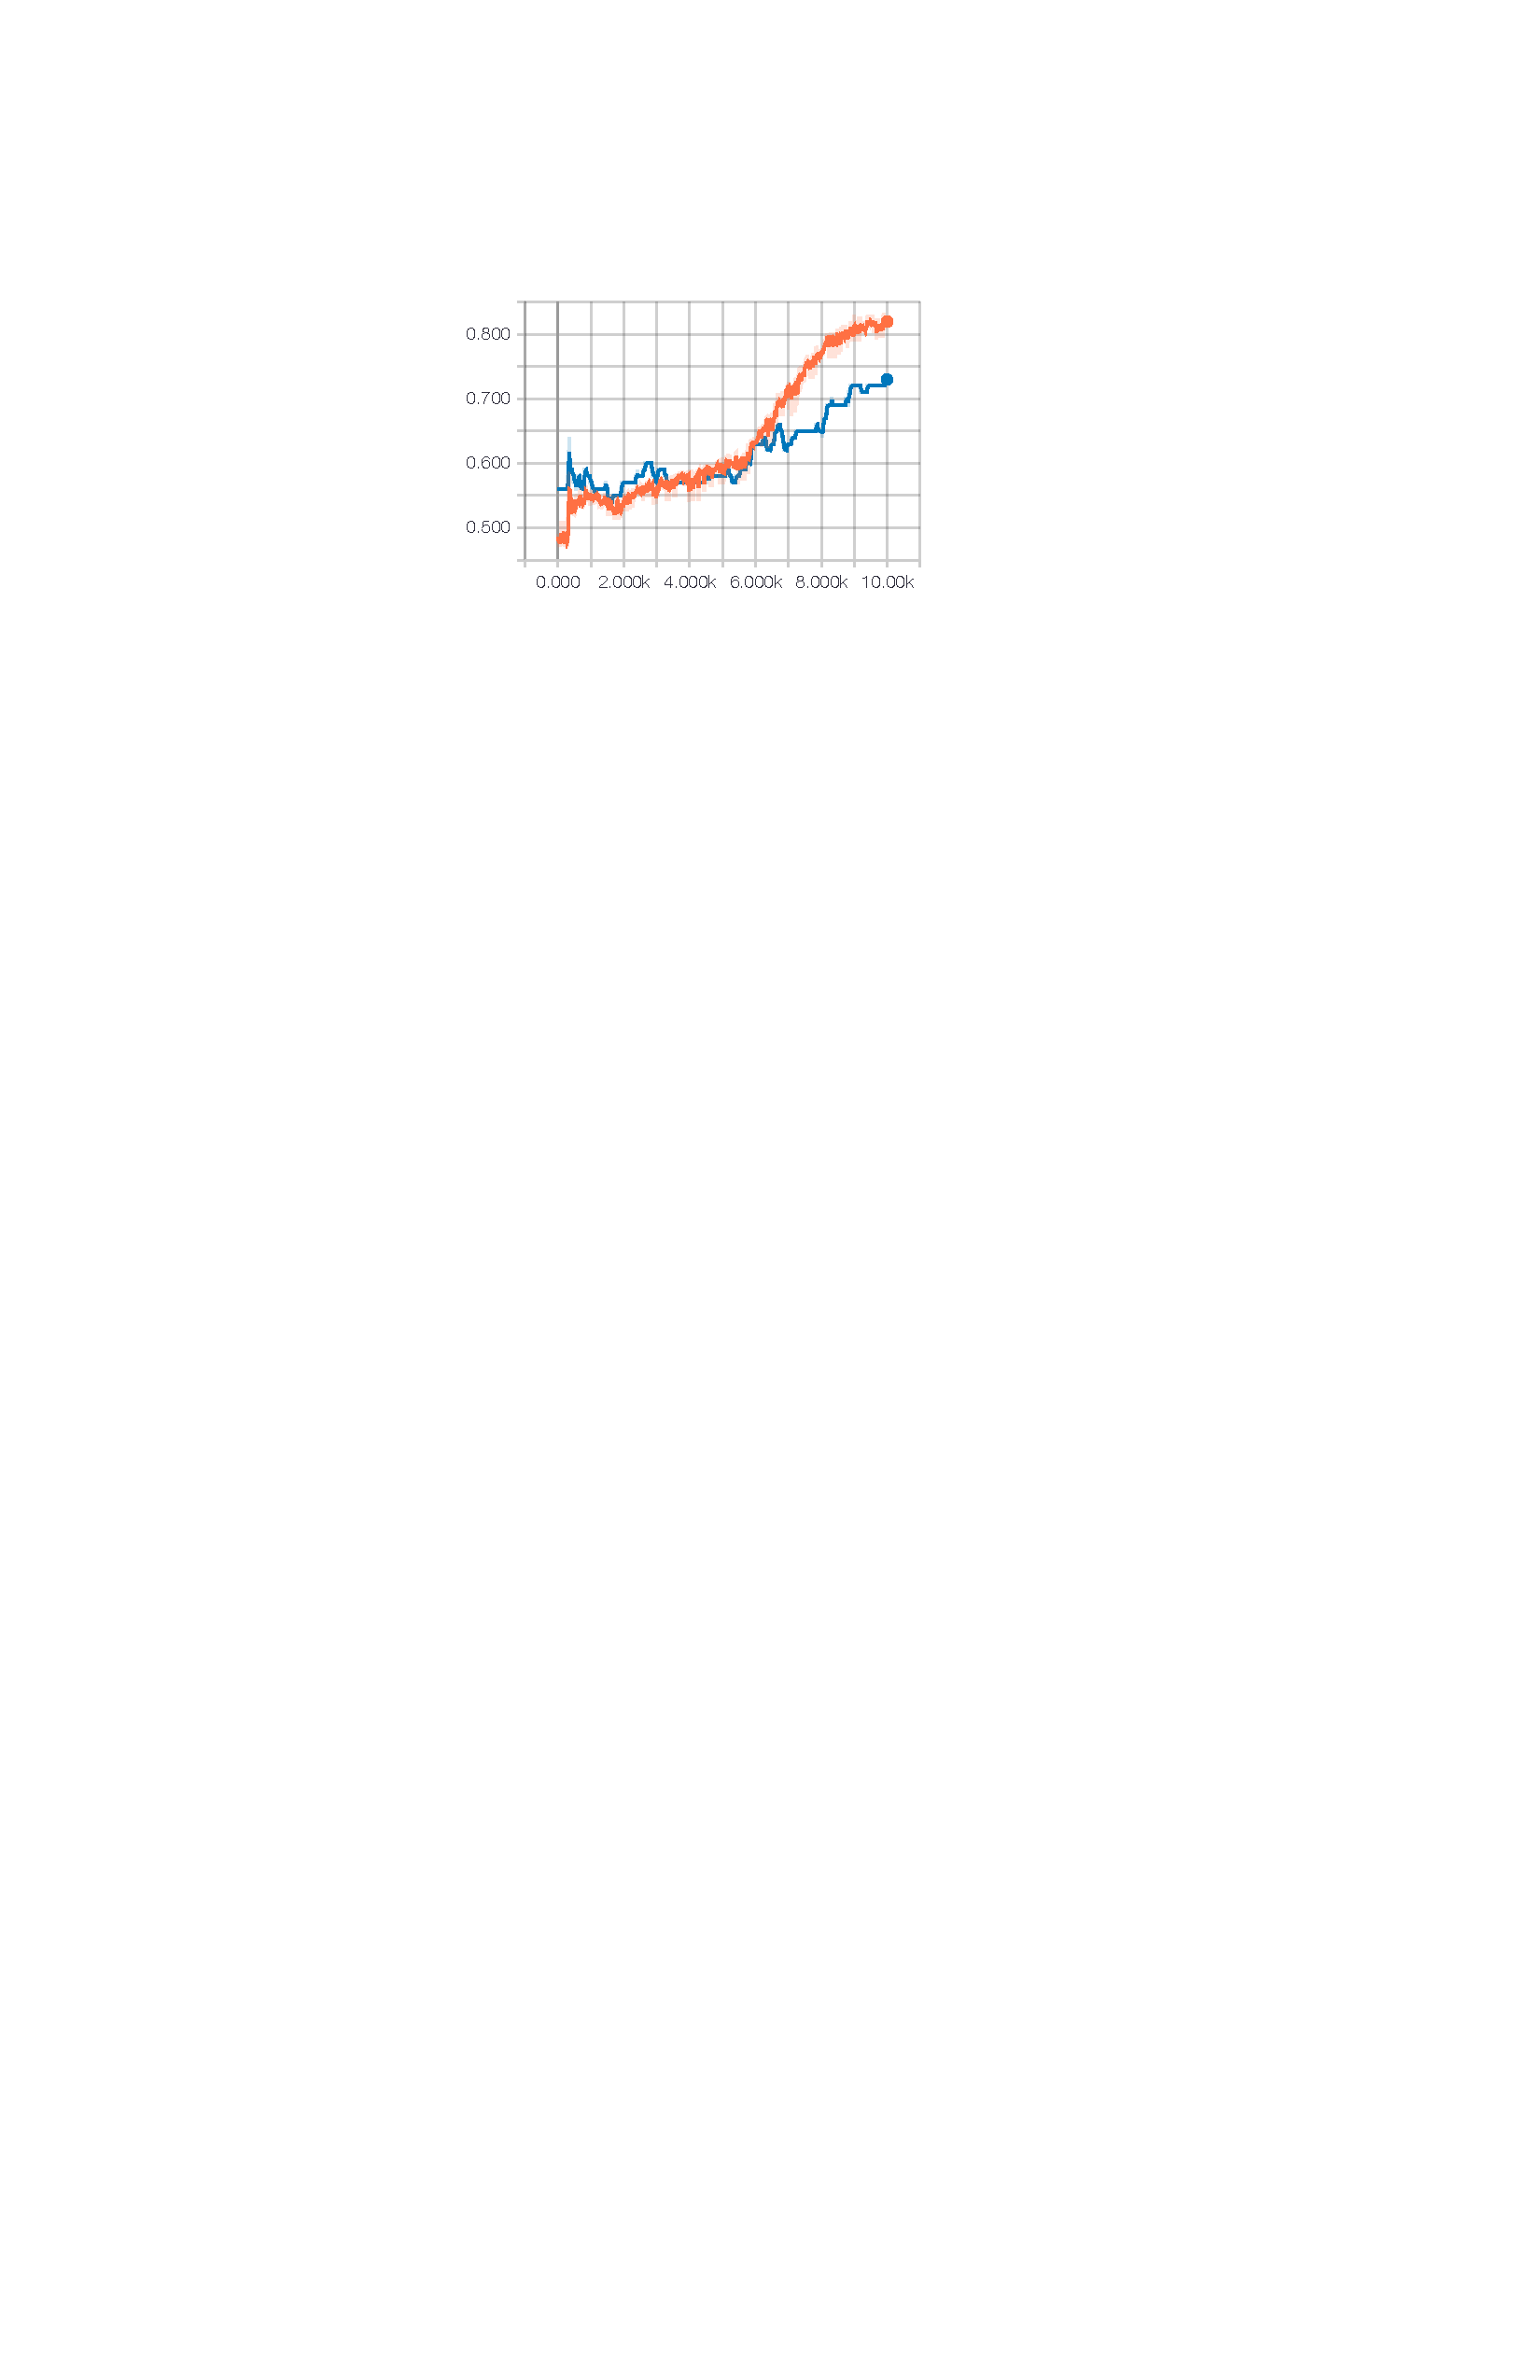
\includegraphics[width=0.45\textwidth]{img/mlaccuracyt1.pdf}}
        % \includesvg[width=0.45\textwidth]{img/accuracy.svg}}
    \subfigure[Loss]{
        \label{fig:mlt1loss}
        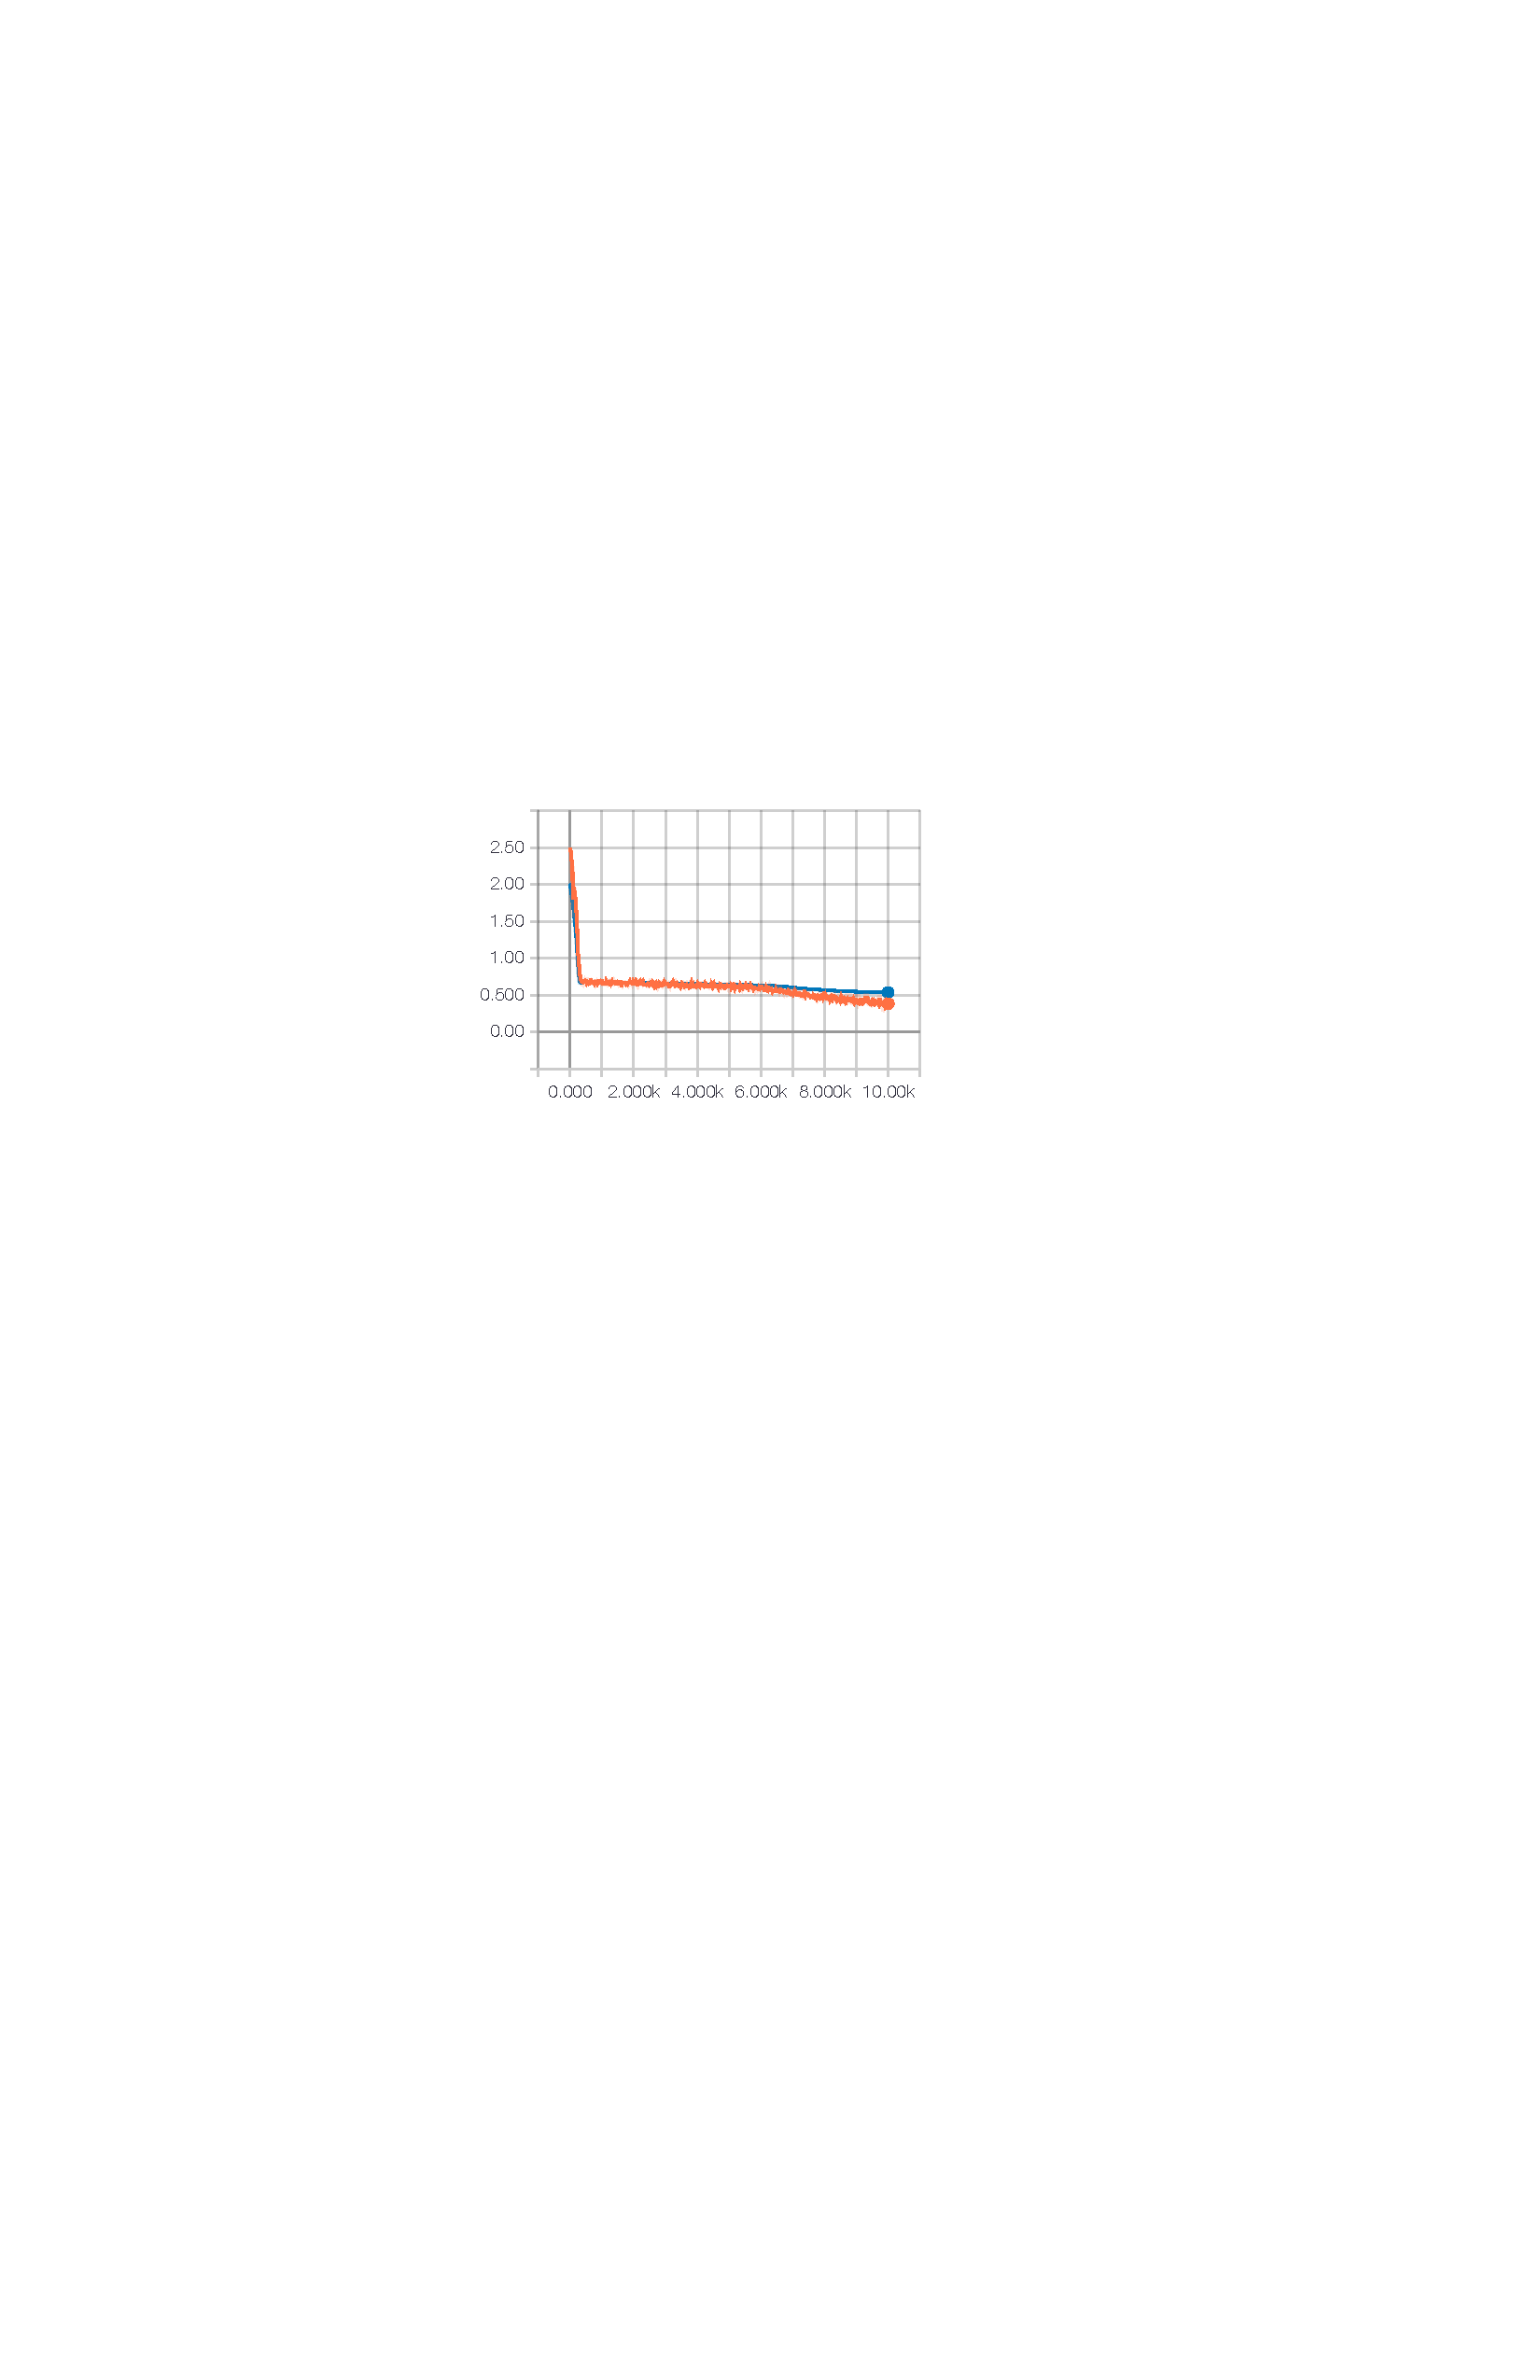
\includegraphics[width=0.45\textwidth]{img/mllosst1.pdf}}\\
    \subfigure[Precision]{
        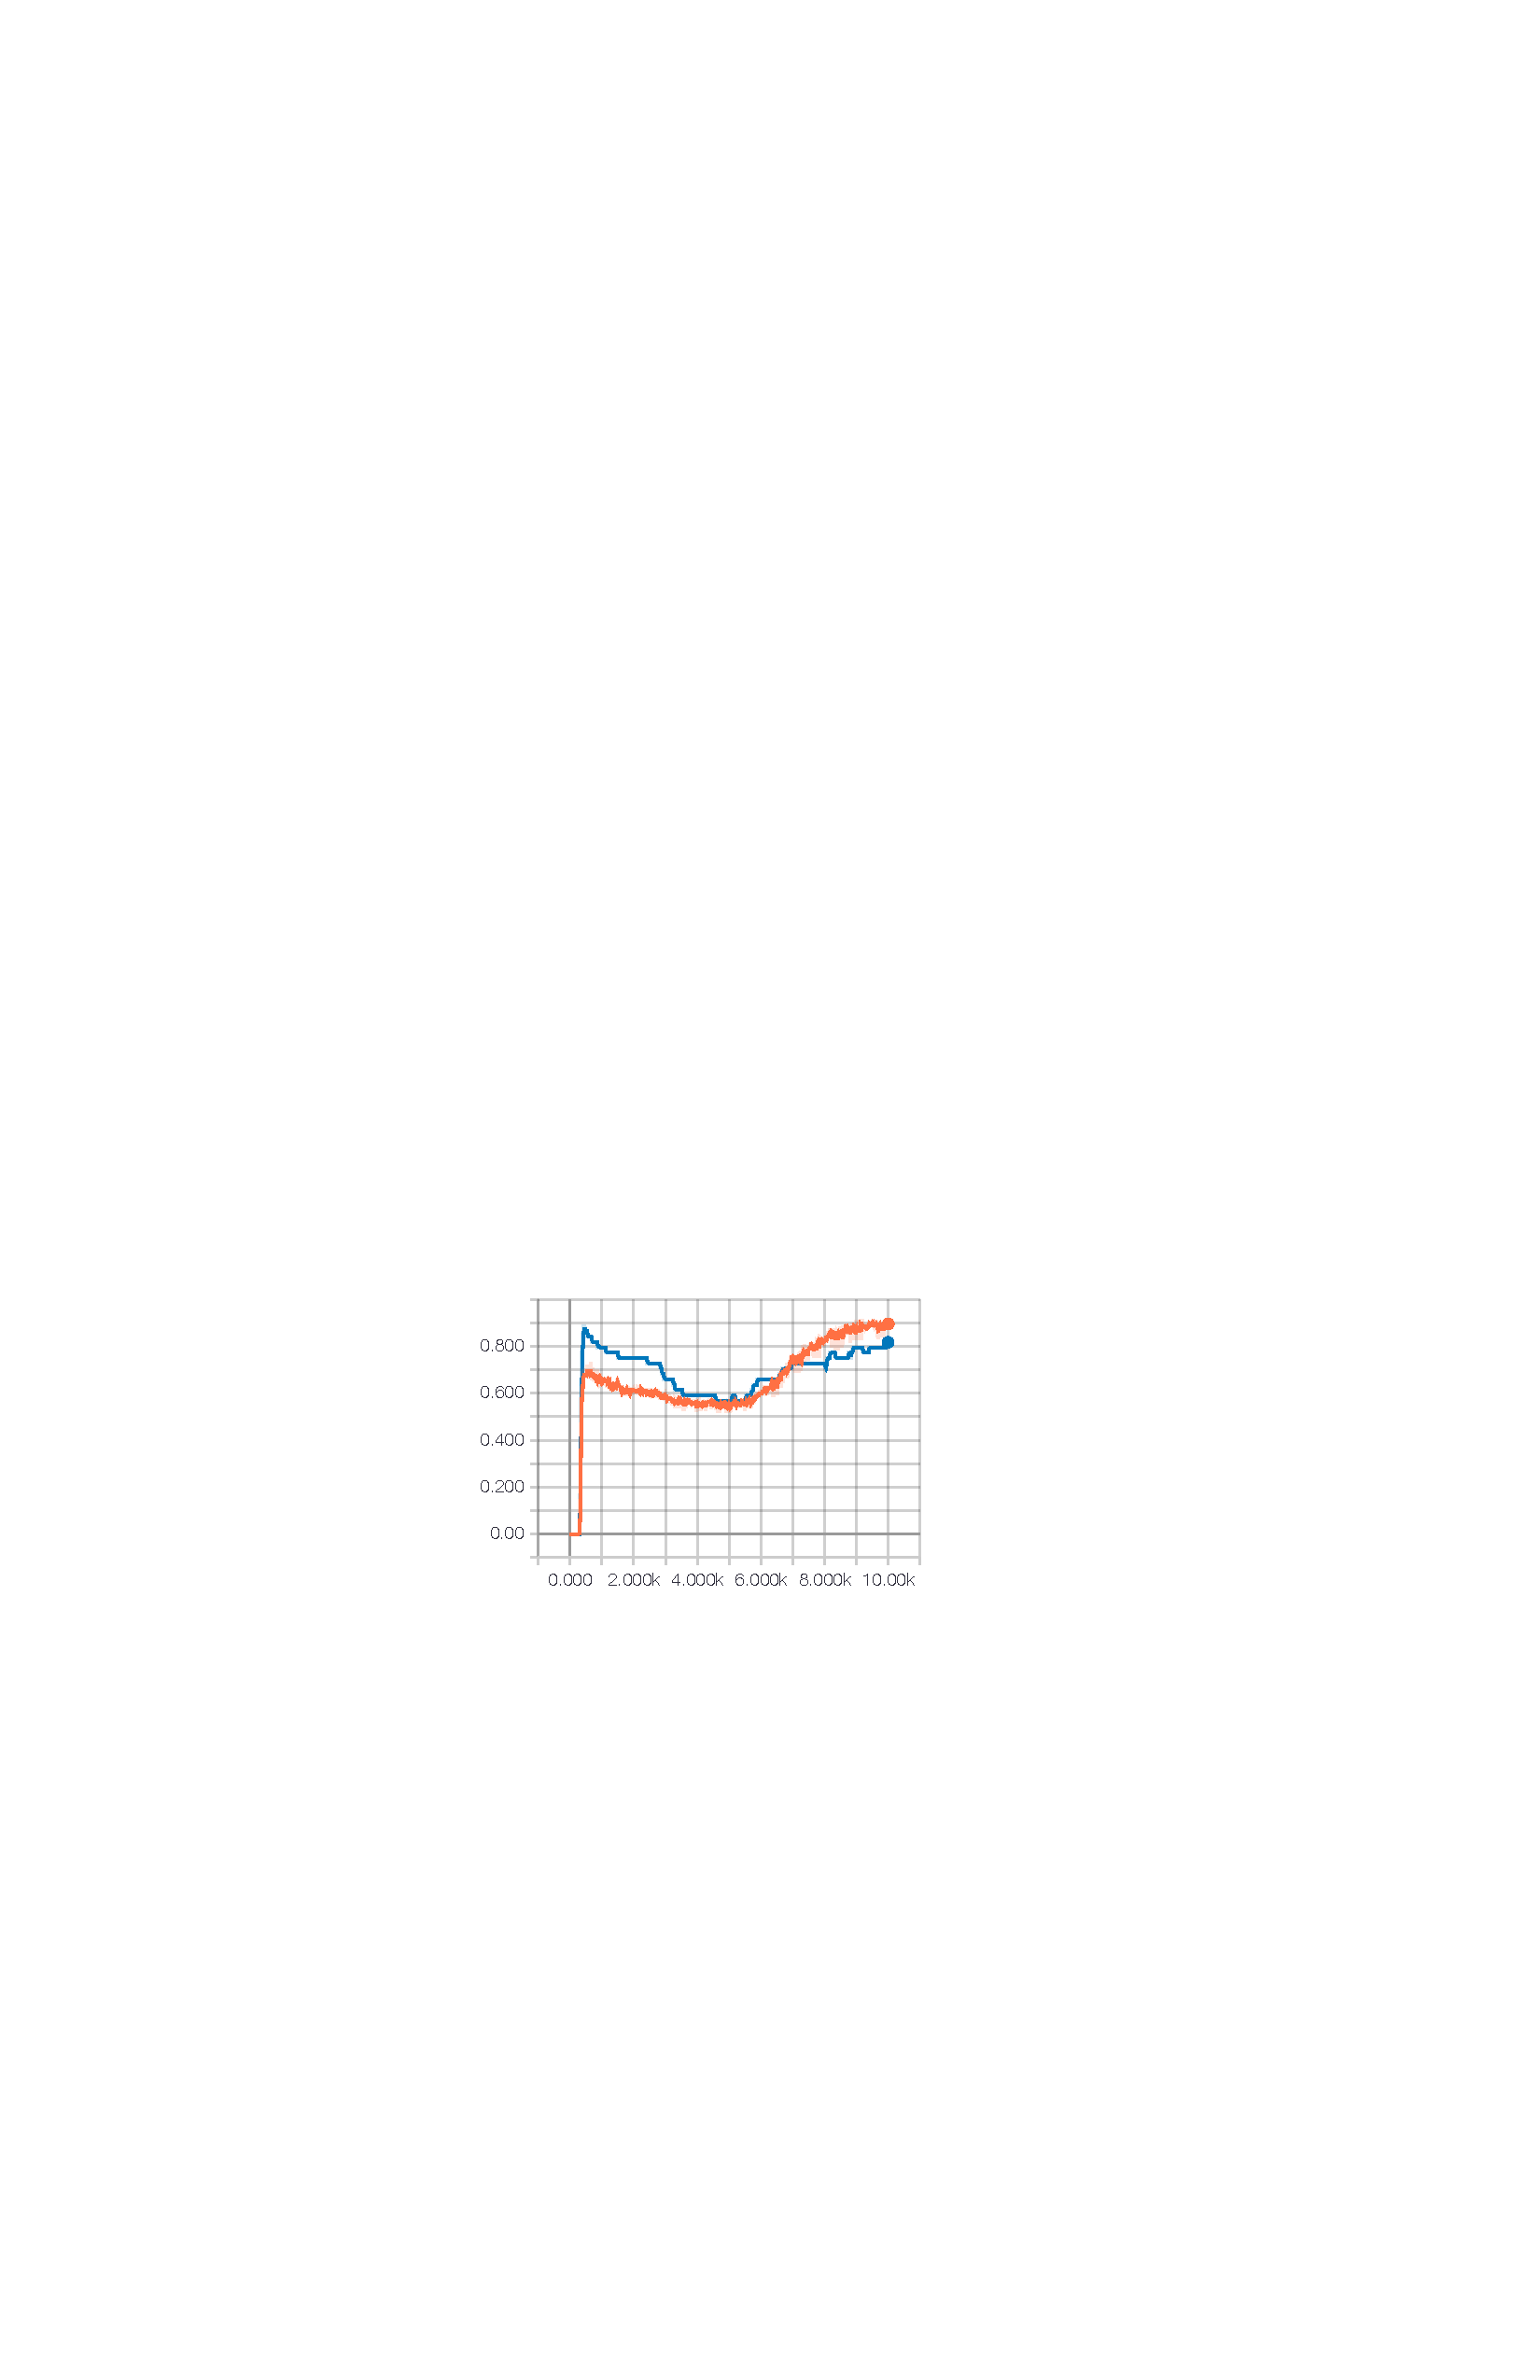
\includegraphics[width=0.45\textwidth]{img/mlprecisiont1.pdf}}
    \subfigure[Recall]{
        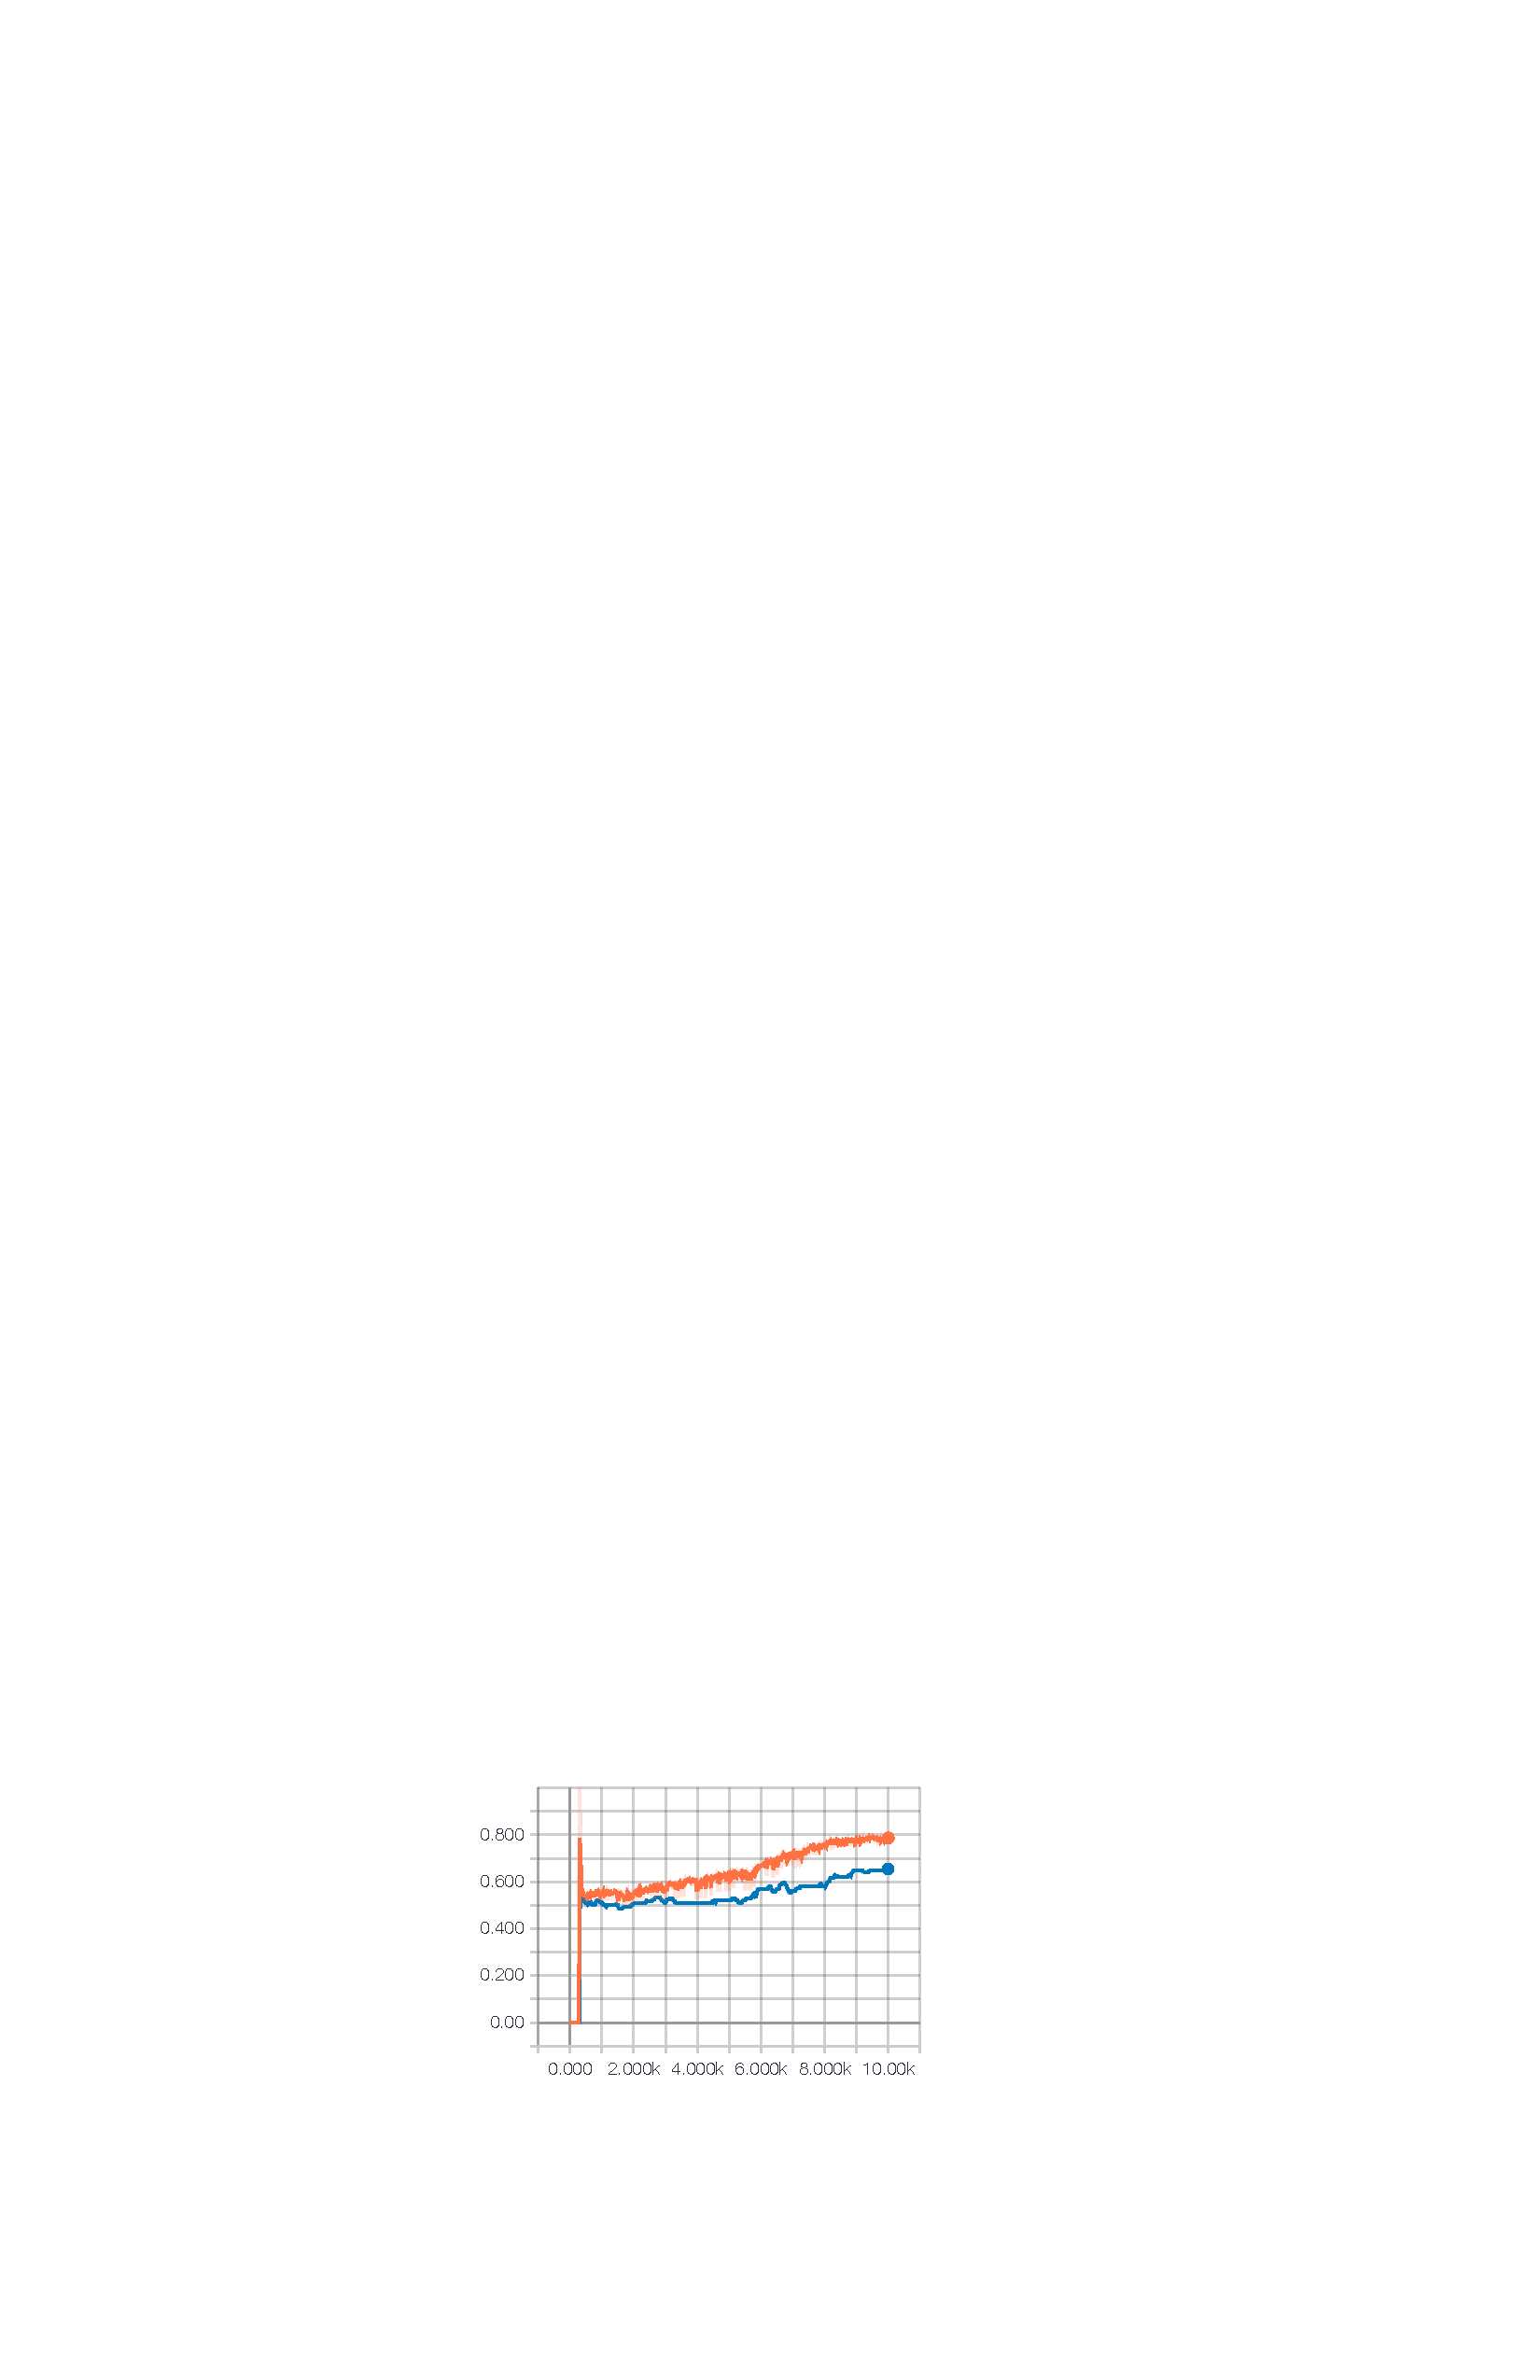
\includegraphics[width=0.45\textwidth]{img/mlrecallt1.pdf}}
    \caption{Metrics for test training sample}
    \label{fig:mlt1}
\end{figure}


\subsection{Project Progress}
The whole project is mainly divided into three parts.
Each phase took around 2 months.
The first part is concentrated on the literature review and prepare the knowledge about machine learning (detail will be included in Section \ref{sec:learning}).
\begin{itemize}
    \item Literature review about bisimulation
    \item Literature review about machine learning on logic
    \item Learn to use packages
    \item Plan and design the project
\end{itemize}
The second part is to develop a bisimulation algorithm and a test cases generator.
\begin{itemize}
    \item Review relevant work on bisimulation
    \item Implement the standard algorithm
    \item Develop the visualisation tool
    \item Test and adjust the developed algorithm
    \item Develop the test case generator 
    \item Test and adjust the generator 
\end{itemize}
The last part is to construct the machine learning algorithm and experiment.
\begin{itemize}
    \item Review relevant work on the logical learning in neural network 
    \item Learn to use TensorFlow 
    \item Implement the neural network 
    \item Test the network and adjust the hyper-parameters
    \item Experiment on different cases (to be seen in Section \ref{sec:experiment})
\end{itemize}
For the timeline of the project, Gantt-chart is given below in Figure \ref{fig:ganttchart}.

\begin{figure}[hp]
    \centering
    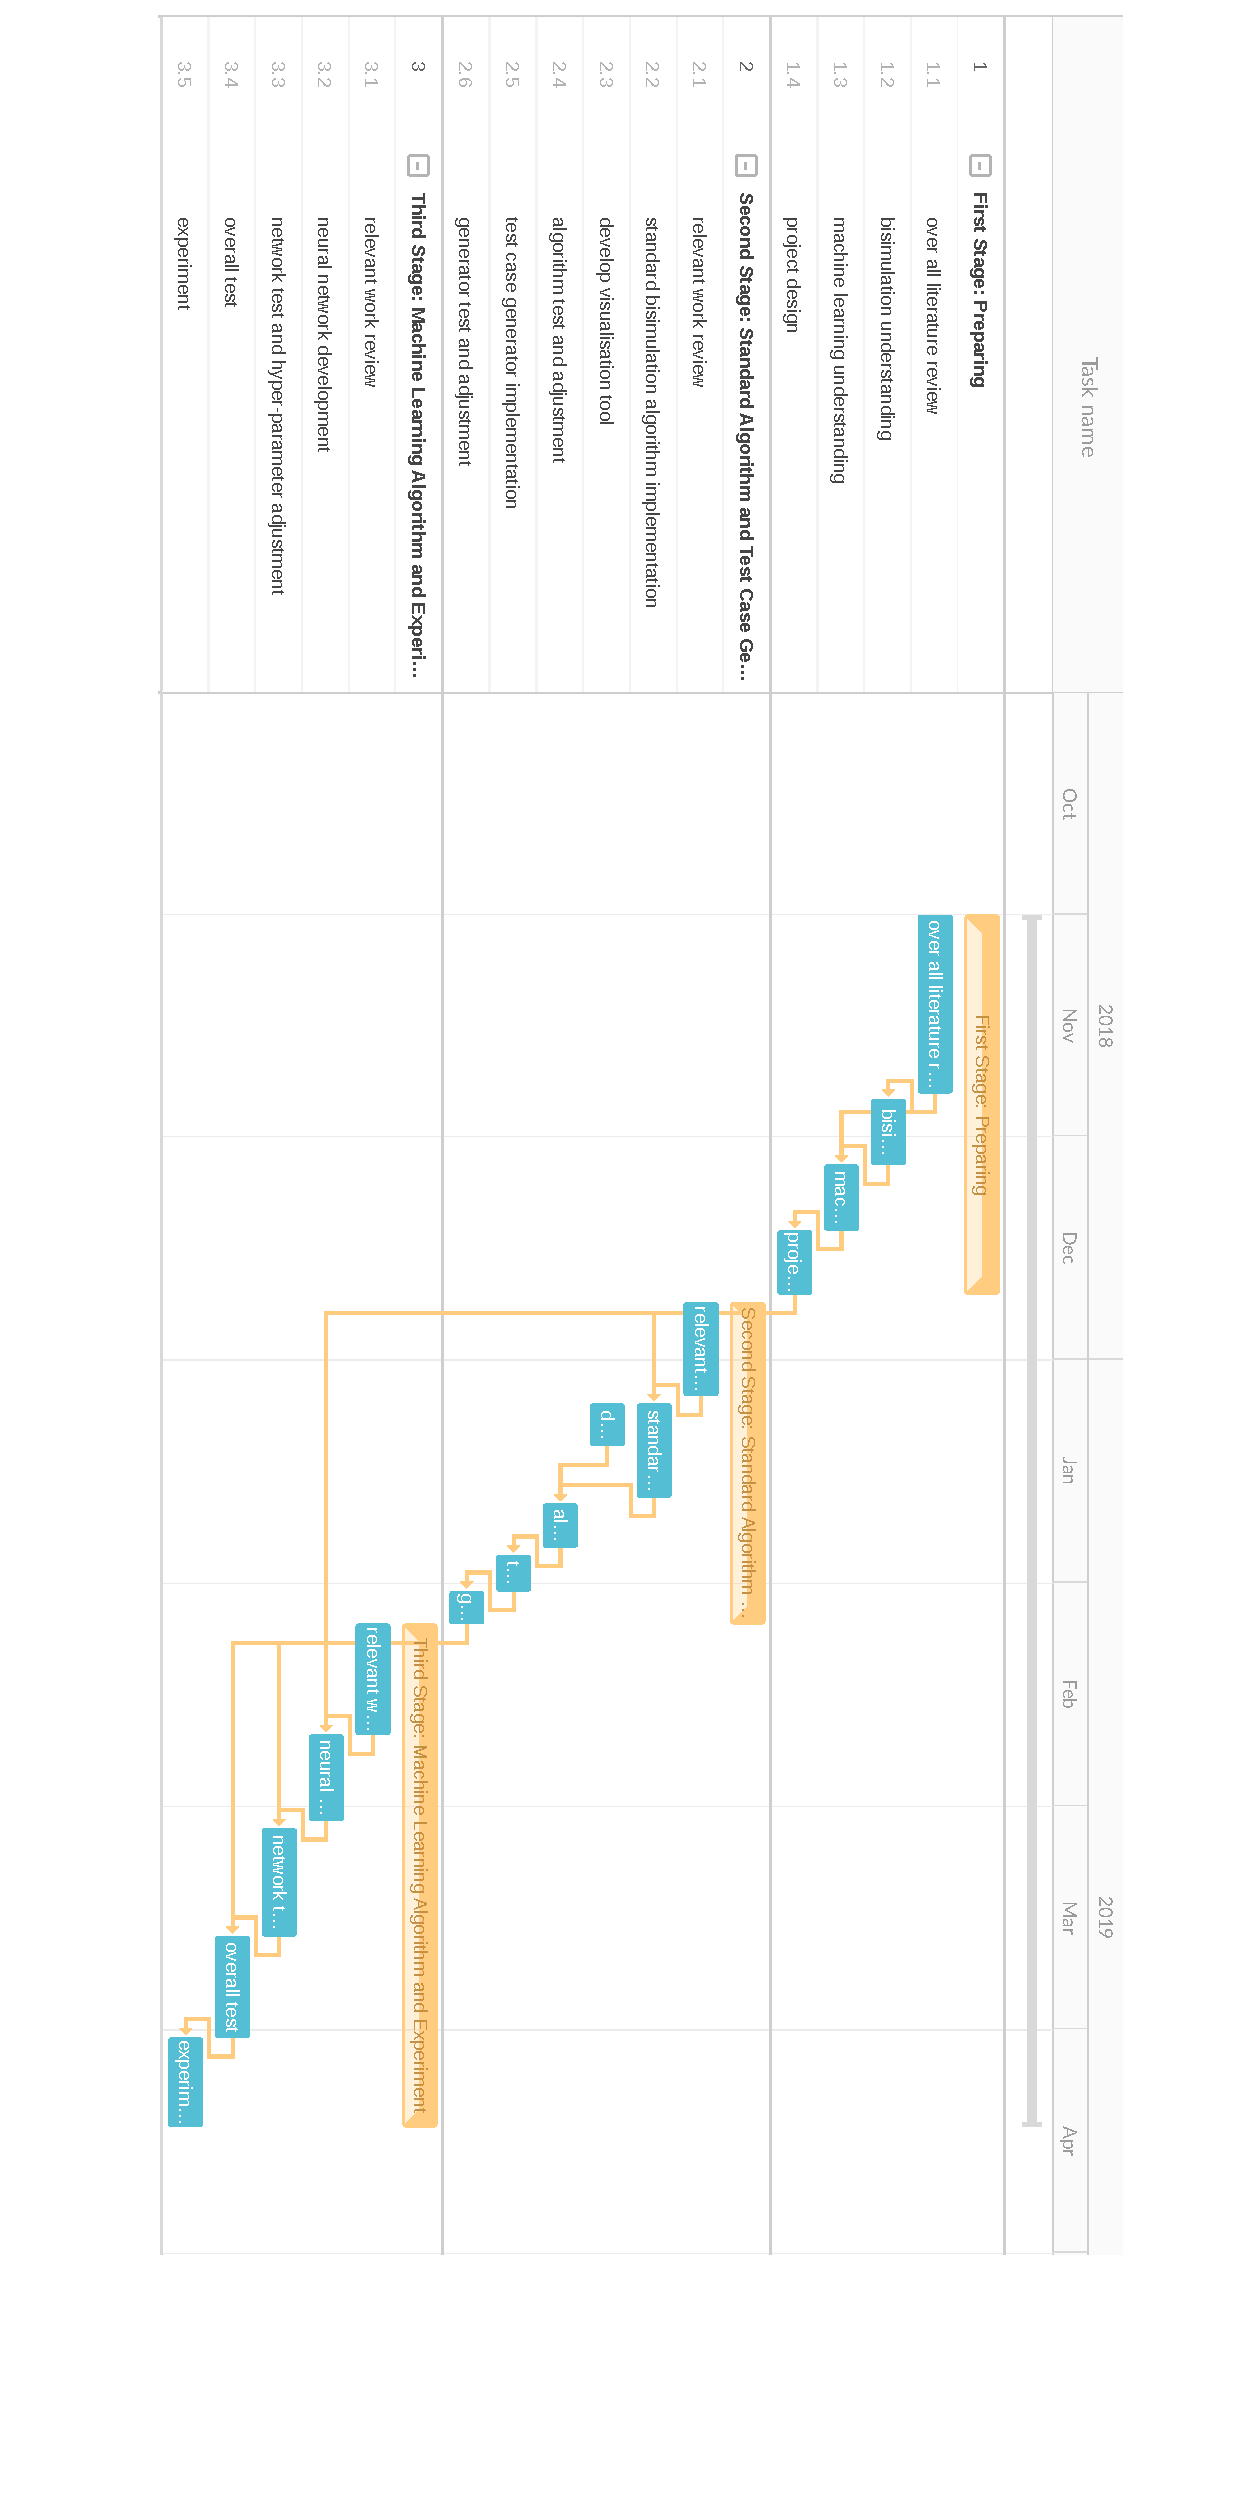
\includegraphics[height=\textheight]{img/gantt.pdf}
    \caption{Gantt Chart}
    \label{fig:ganttchart}
\end{figure}






\subsection{Environment}
\subsubsection*{Hardware}
2012 Mac mini computer, with processor Core i5 (i5-3210M), 8GB RAM is used during the developing of the project.
When comes to the experiment, it is run on the Google Cloud Platform with 2 standard vCPUs (virtual CPU), 7.5 GB RAM and one NVIDIA Tesla K80 GPU.
\subsubsection*{Software}
This project is developed on \texttt{PyCharm 2018.3.6}, under \texttt{macOS Mojave 10.14}.
For the main packages/library used in the project, \texttt{NetworkX 2.2} is used to manipulate the graph objects.
The visualisation of the graphs is based on \texttt{ Matplotlib 2.2.3}.
Neural network and relevant training is based on the \texttt{TensorFlow 1.12.0} and \texttt{TensorFlow-GPU 1.12.0}.
For the experiment the project is running under \texttt{Ubuntu 16.04.6 LTS}.
\section{Experiment}
\label{sec:experiment}
In this section, the design, realization and the result of experiments will be stated.
Due to the relatively large scale test is needed, experiments are deployed on Google Cloud Platform. 
In addition, the experiments run on \texttt{TensorFlow-GPU 1.12.0} rather than CPU version, which is used during the development.
Consequently the result there may be slightly different.

\subsection{Design}
The aim of the experiments is to explore the capability of the network for understanding the logical feature.
The experiment is designed into two parts.
The first part is designed to test the stability of the training with respect to all the possible graphs with the same scale.
So that the reliability of a single test can be estimated.
The reason to estimate the reliability of a single test is that extensive and complete experiments are not feasible when the graph is big, due to the exponential growth of possible graph pairs.
However, even for relatively small graph, generate all possible cases would be very time-consuming. 
And that is also the reason why generate-all-generator was abandoned (see Section \ref{sec:imptestcasegenerator}).
Instead, sampling is chosen as an alternative plan.
Random test case generator can be seen as a sampling machine.
By generate multiple groups of graphs with different density, the sampling is expected to cover most of the combinations.
Specifically, the experiment parameters will be shown in Listing \ref{lst:wideexp}.


% \captionof{listing}{Wide experiments arguments \label{lst:wideexp}}
% \vspace{-0.5em}
\begin{code}
\caption{Wide experiments arguments}
\label{lst:wideexp}
\begin{minted}[linenos, frame=single,breaklines]{python}
# ========== wide experiments ==========
# ---- ARGUMENTS ----
nodes_num = 5 
edge_type_num = 3 
c_type = random 
case_number = 10000 
graph_density = [0.1, 0.2, 0.3, 0.4, 0.5, 0.6, 0.7, 0.8, 0.9]
p_rate = 0.5 
learning_rate = 0.1
epochs = 500
batch_size = 100
# -------------------

\end{minted}
\end{code}

The second part of the experiments is aiming to find the limit of this network, namely the algorithm designed in this project (see Figure \ref{fig:mlp_model}).
In this part, the algorithm will be trained on graphs with different scale, i.e. bigger graphs.
And by comparison, the limitation of the network can be estimated.
Notice that for graphs with different scale, the network will be slightly different, i.e. only the length of the input layer and re-represent layer (see Figure \ref{fig:mlp_model}) will be different.
However, the overall structure will be the same.
Here are the arguments used in this part (see Listing \ref{lst:deepexp}).\vspace{1em}

% \captionof{listing}{Deep experiments arguments \label{lst:deepexp}}
% \vspace{-0.5em}
\begin{code}
\caption{Deep experiments arguments}
\label{lst:deepexp}
\begin{minted}[linenos, frame=single,breaklines]{python}
# ========== deep experiments ==========
# ---- ARGUMENTS ----
nodes_num = [5, 6, 7, 8, 9, 10, 11, 12, 13, 14] 
edge_type_num = 3 
c_type = random 
case_number = 10000 
graph_density = 0.5
p_rate = 0.5 
learning_rate = 0.1
epochs = 500
batch_size = 100
# -------------------
\end{minted}
\end{code}

\subsection{Results}
\label{sec:results}
All the test will be run for multiple times to avoid potential coincidence.
They will be uploaded including the full raw data of training, trained model and all the metrics logged during the training.
Here we only give two results to make sure the characteristic can be identified easily.

\subsubsection*{Wide Experiment}
For the wide experiment, the accuracy and loss of two duplicate experiments are given in Figure \ref{fig:resw12}.
Notice that in order to make graphs more clear, only the cases generated with \texttt{graph\char`_density = 0.1, 0.3, 0.5, 0.7, 0.9} (see Listing \ref{lst:wideexp}) are shown in the graphs. 
Also, all the metrics here is base on the test set rather than the training set.
Each line in the chart stands for one training.
The legend shows the parameter of the train.
For example, \texttt{random\char`_n5\char`_e3\char`_10000\char`_gd0.1\char`_p0.5\char`_test} means the corresponding training data is generated by the random generator.
The graphs represented has 5 nodes, 3 types of edge with an average 0.1 graph density.
And this accuracy is calculated base on the test data set.
Notice that ``graph density" used here is not a strict mathematical concept. 
It only stands for the degree of how dense the graph is (see Algorithm \ref{alg:R_tcg}).
The size of the test case is 10000. 
The rate between negative cases and positive cases is around 0.5.

\begin{figure}[h]
    \centering
    \subfigure[Wide experiment 1: accuracy]{
        \label{fig:exp11acc}
        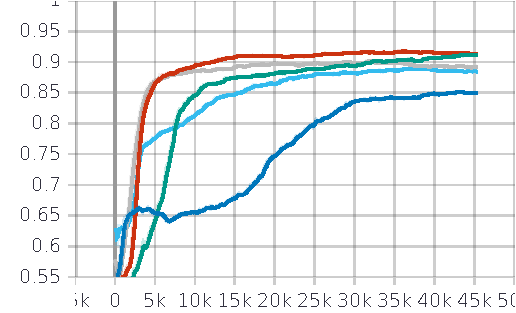
\includegraphics[width=0.45\textwidth]{img/exp11acc.pdf}}
    \subfigure[Wide experiment 2: accuracy]{
        \label{fig:exp12acc}
        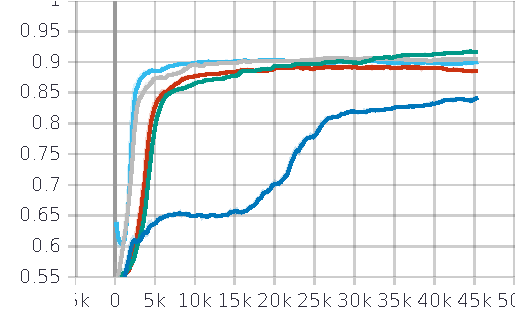
\includegraphics[width=0.45\textwidth]{img/exp12acc.pdf}}
    \subfigure[Wide experiment 1: loss]{
        \label{fig:exp11loss}
        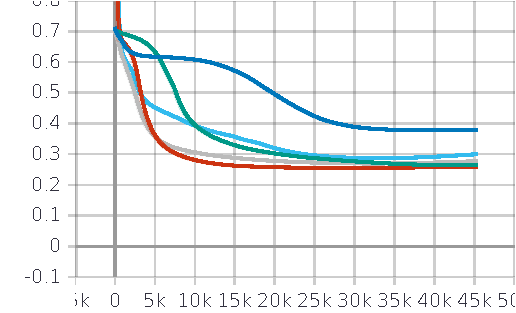
\includegraphics[width=0.45\textwidth]{img/exp11loss.pdf}}
    \subfigure[Wide experiment 2: loss]{
        \label{fig:exp12loss}
        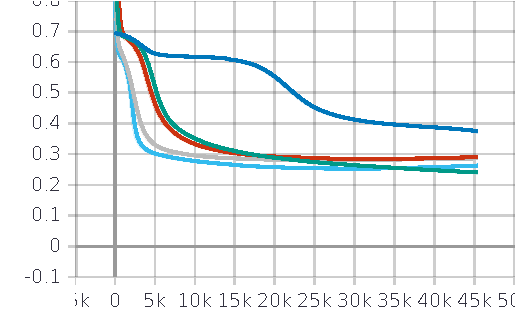
\includegraphics[width=0.45\textwidth]{img/exp12loss.pdf}}
    \subfigure[Legend]{
        \label{fig:legendexp1}
        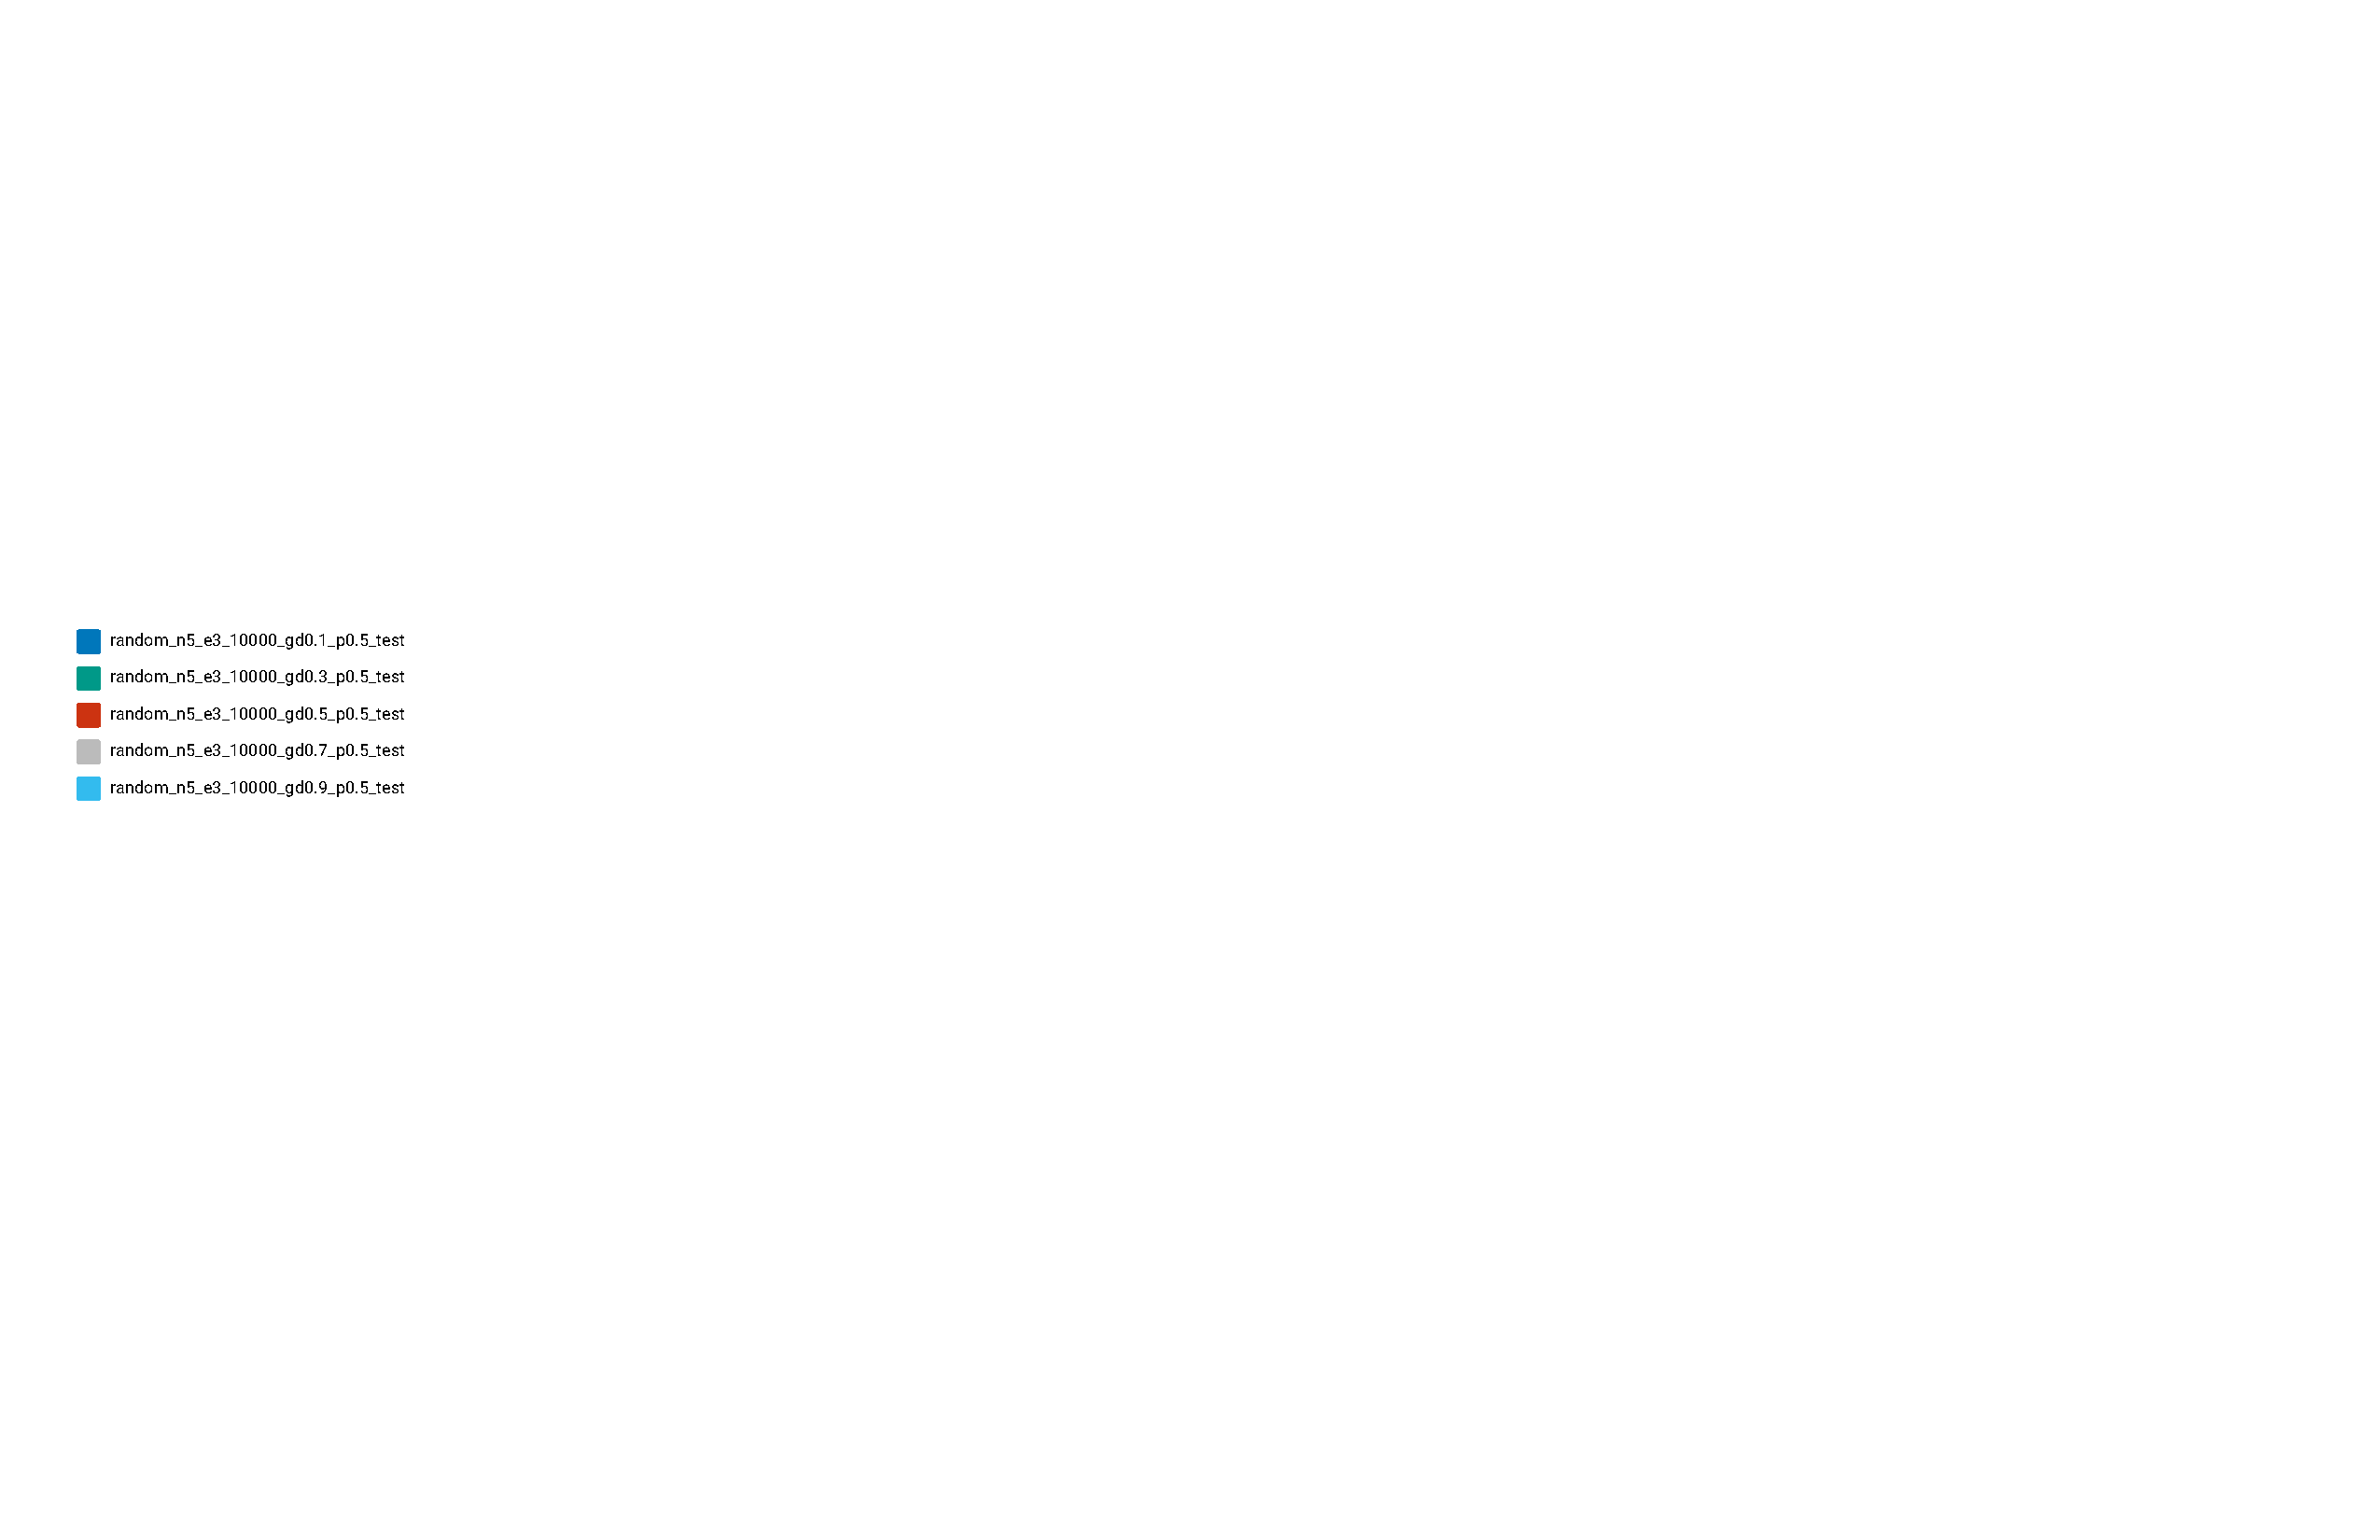
\includegraphics[width=0.4\textwidth]{img/legendexp1.pdf}}
    \caption{Result of wide experiment 1 and 2}
    \label{fig:resw12}
\end{figure}

The first conclusion is that this kind of neural network can learn the logical concept like bisimulation.
Most cases showed approximately 85\% accuracy when 500 epochs end.
This reveals the train is successful and the network actually catches the concepts of bisimulation.
Compare all training, the graphs with 0.1 as density (i.e. most sparse) are harder for the network to be trained.
Intuitively, the graphs with more link can express more complicated logic.
And should be harder for the network to learning the feature.
However, it may because the dense graph will show less complicate bisimulation propriety.
In other words, when the graph becomes denser, the bisimulation pattern may go more simple.
Concretely, for a dense graph, the mini bisimilar equivalent graph will most likely be either completely same (e.g. Figure \ref{fig:outputg3}) or be one node with self-loop of all possible link (e.g. Figure \ref{fig:outputg4}).
For the first situation, two bisimilar graphs will be isomorphic (i.e. nodes of two graph are connected in the same way, only the sequence of the nodes is different).
In this situation, the problem turns to distinguish if two graphs are isomorphic, which is much easier.
For the second situation, the graph can be represented in a graph with one node.
In this situation, the graphs are bisimilar may be diverse.
But graphs that are not bisimilar may have a big difference which will make the task easier.

The wide experiment can guide the deep experiment.
The result of wide experiment indicates that using random test case generator sample form the space of possible graphs is practicable (i.e. the performance of the algorithm when feeding dataset generated by one generator is representative).
Because, except the one training (i.e. generator has 0.1 as density), most training show similar results.
It reveals that the result of training for graphs with a certain scale can be represented by the training that bases on the data generated by a random test case generator.

\subsubsection*{Deep Experiment}
The purpose of the deep experiment is to test the capability of the neural network.
Thus in this experiment, graphs used here will be larger (i.e. has more nodes while maintaining the same number of edge type).
According to the learning curve and where the accuracy converges, the capability of this neural network can be estimated.

In this experiment, only the number of nodes for the generated graphs will change (see Listing \ref{lst:deepexp}). 
And the \texttt{graph\char`_density} will be 0.5.
Since in the wide experiment, the test cases generated with 0.5 graph density can better represent the overall leaning states (see Figure \ref{fig:resw12}).

\begin{figure}[h]
    \centering
    \subfigure[Deep experiment 1: accuracy]{
        \label{fig:exp21acc}
        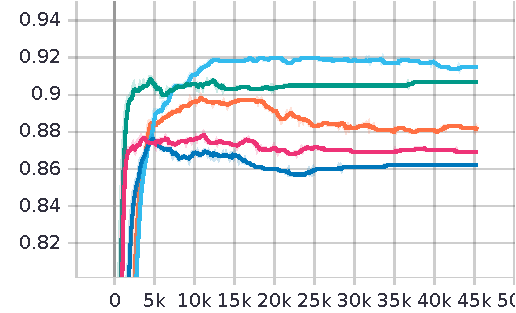
\includegraphics[width=0.45\textwidth]{img/exp21acc.pdf}}
    \subfigure[Deep experiment 2: accuracy]{
        \label{fig:exp22acc}
        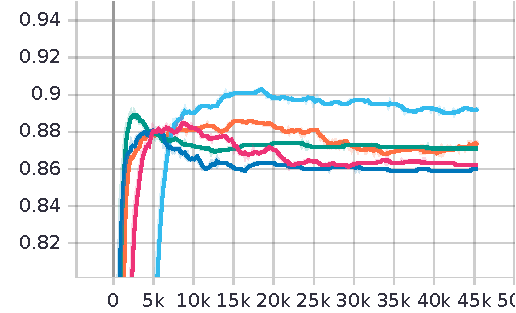
\includegraphics[width=0.45\textwidth]{img/exp22acc.pdf}}
    \subfigure[Deep experiment 1: loss]{
        \label{fig:exp21loss}
        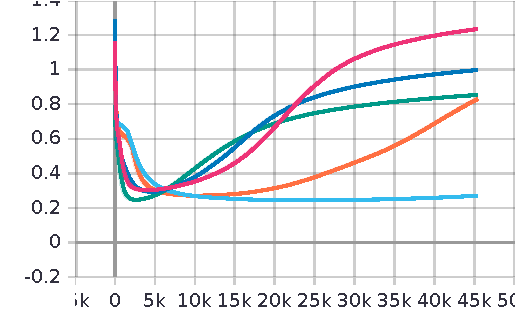
\includegraphics[width=0.45\textwidth]{img/exp21loss.pdf}}
    \subfigure[Deep experiment 2: loss]{
        \label{fig:exp22loss}
        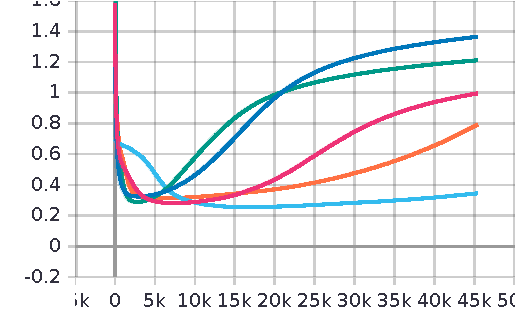
\includegraphics[width=0.45\textwidth]{img/exp22loss.pdf}}
    \subfigure[Legend]{
        \label{fig:legendexp2}
        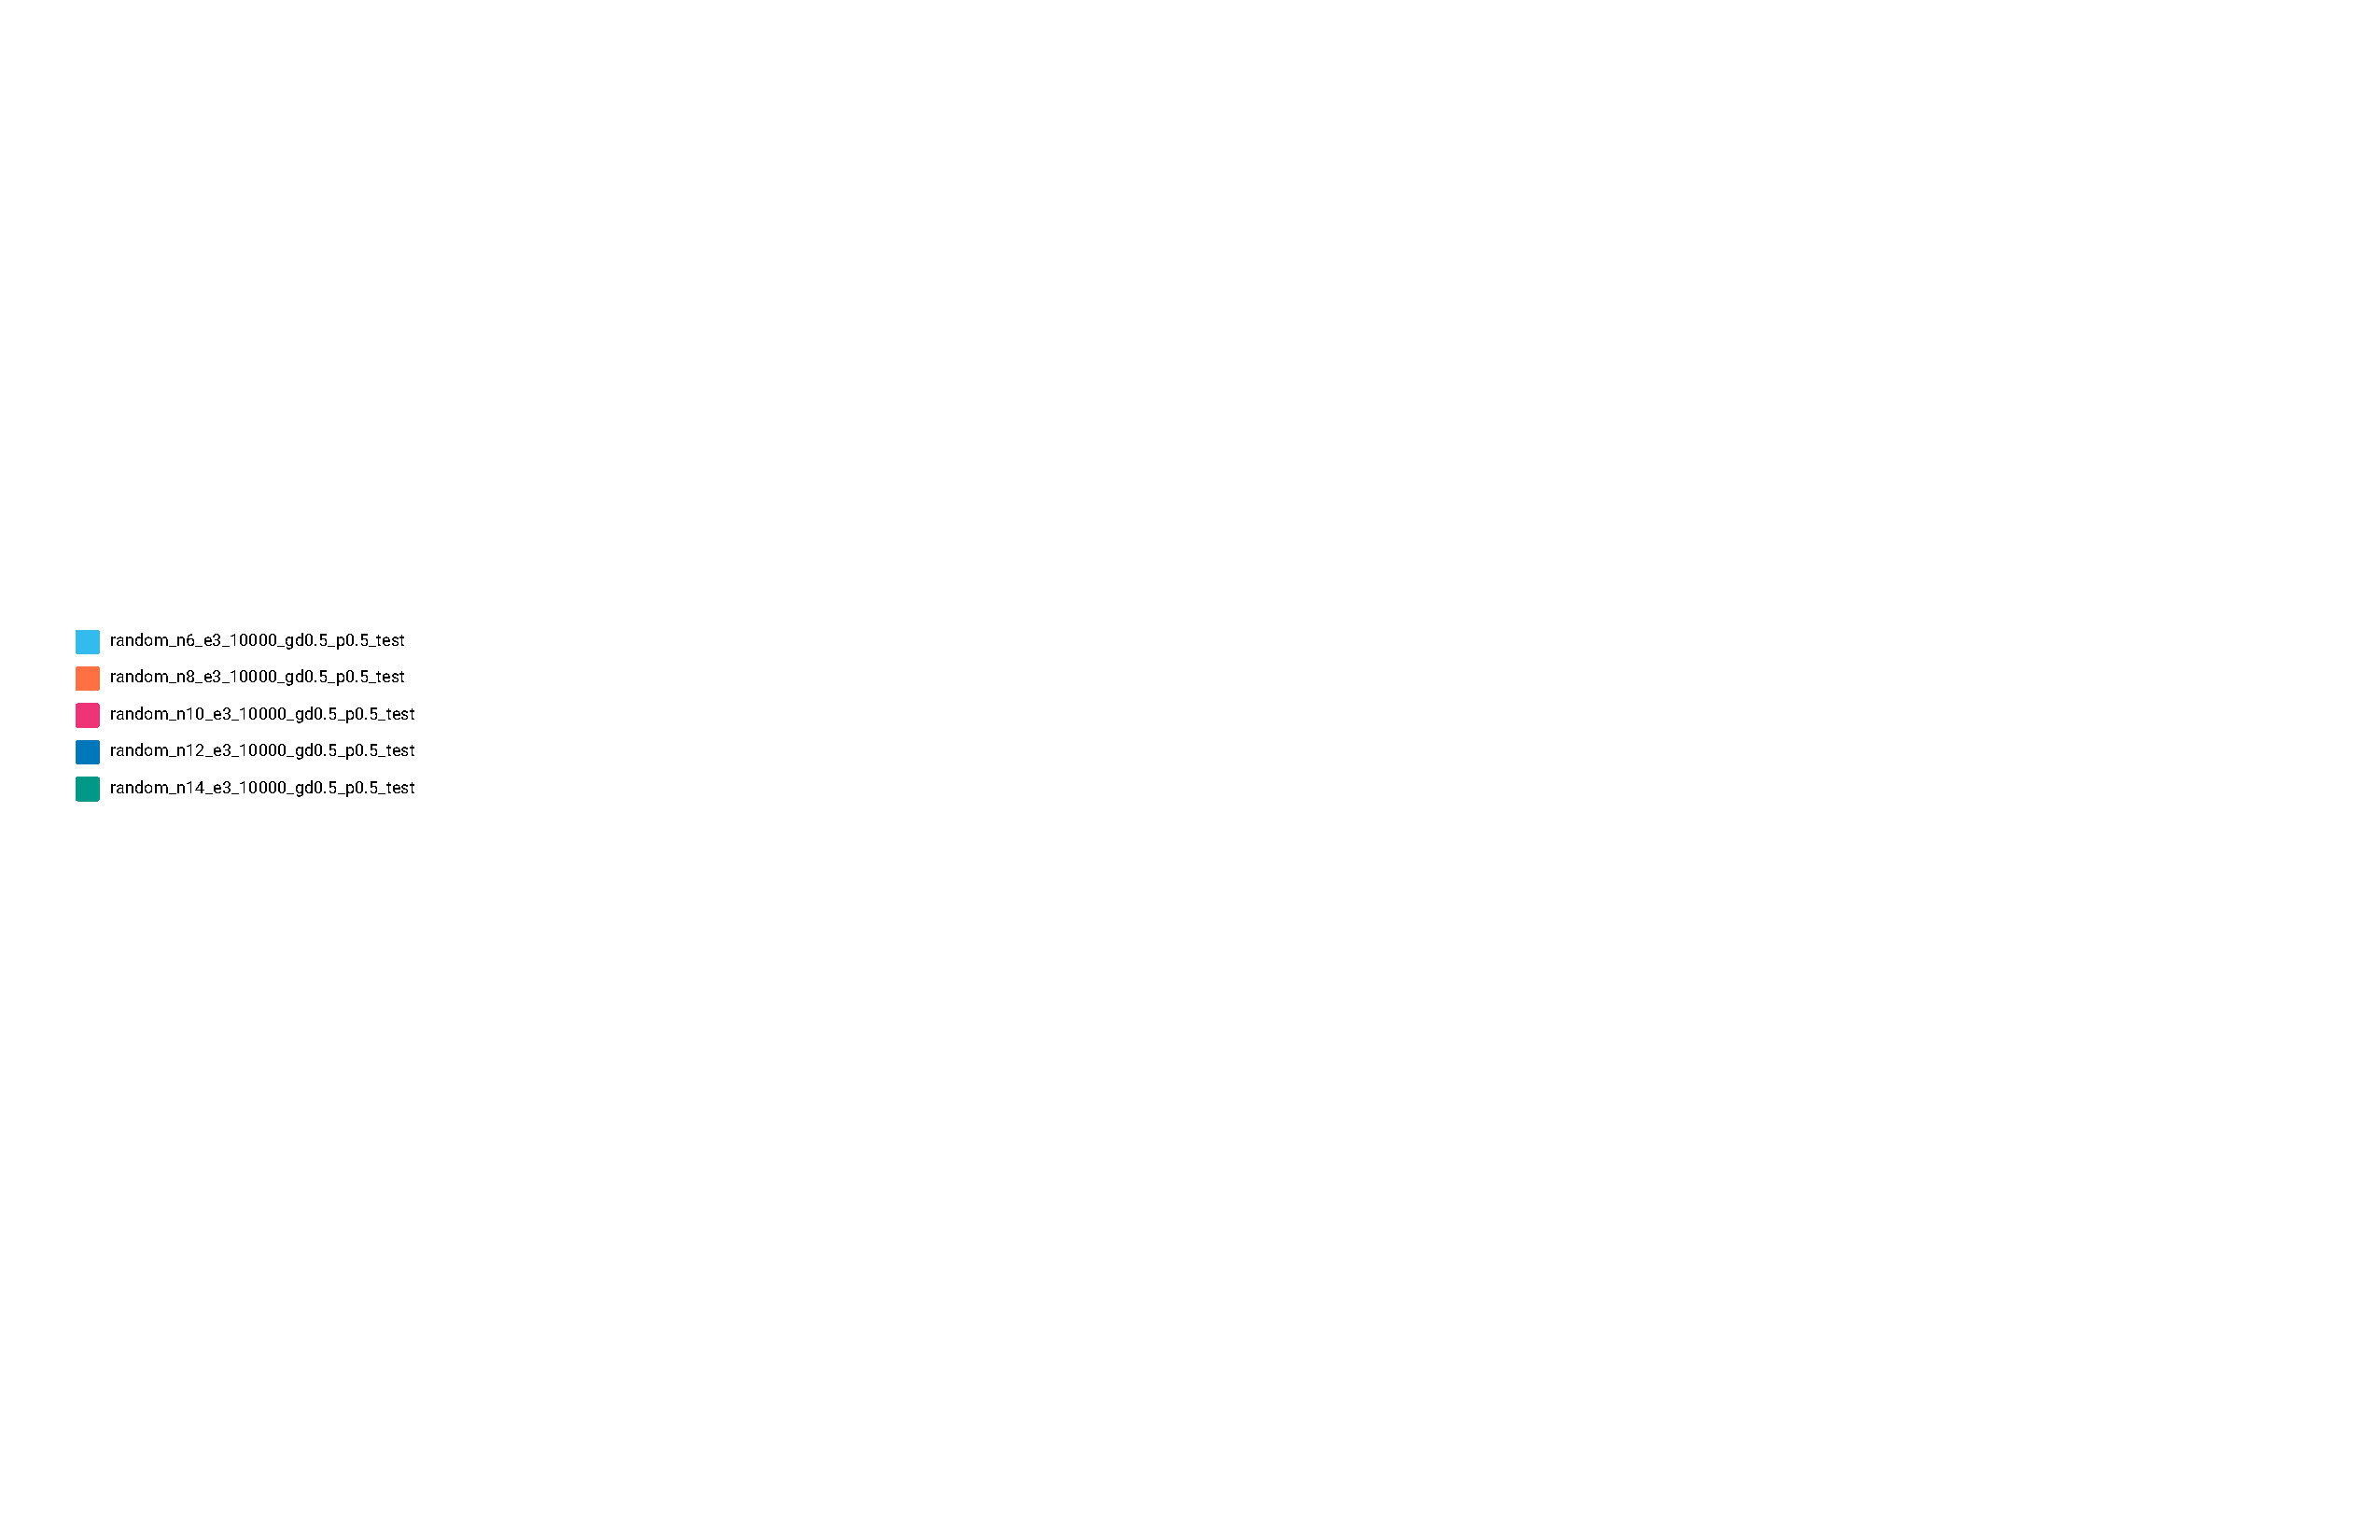
\includegraphics[width=0.4\textwidth]{img/legendexp2.pdf}}
    \caption{Result of deep experiment 1 and 2}
    \label{fig:resd12}
\end{figure}

The result is shown in Figure \ref{fig:resd12}.
Same as the wide experiment, in order to make graphs more clear, only the cases generated with \texttt{nodes\char`_num = 6, 8, 10, 12, 14} are shown in the graphs.
The model show the sign of overfitting, i.e. the learner start to learn very specific random features rather than the target feature.
Specifically, in the process of training, the loss of training set decreases while the loss on the test set is increasing.
Similarly, the accuracy becomes better on the training set, but worse on the test set.

While it also shows some interesting result which is unexpected.
For the aspect of training result, the value of accuracy will be compared.
Considering the overfitting, the accuracy will drop when training performed too much.
And for different training cases, the point of overfitting is different.
To reduce the effect of the overfitting, the peak of each line will be taken for comparison.
Form Table \ref{tab:pnl} and Figure \ref{fig:expdchart}, except for the case with 14 and 13 nodes, other cases show that accuracy is negatively correlated with the node number.
In other words, when the graphs are larger, it is harder for the network to infer bisimulation.
However, this correlation is not very significant. 
The differences between them are only around 10\%.
This may be caused by the small difference of the network.
Because, when facing different size of graphs, the input layer will increase the size in order to handle it.
It enhances the processing power of the network.
Yet there is still abnormality when it comes to the case of 13, 14 nodes.
This may be because of the quantity of the data.
Because the number of the possible graphs pairs explode from $2^150$ to $2^1176$.
And the quantity of the data is still 10000 groups.
Regarding the random generator as a sampling machine, for a much bigger space, the average difference of the two graphs took randomly will greater.
But the bisimilar pairs generated will be much similar.
Therefore, if the quantity of sampling is greater, the result may be more ``normal".
Since there will be more misleading cases.

From the training process, the graph with fewer nodes is hard to be learned.
The accuracy of the graph with least nodes (i.e. \texttt{random\char`_n6\char`_e3\char`_10000\char`_gd0.5\char`_p0.5\char`_test}) always converge slower than other cases.
But the accuracy of graph with most nodes (i.e. \texttt{random\char`_n14\char`_e3\char`_10000\char`_gd0.5\char`_p0.5\char`_test}) always increase fast than other.
Usually, the network with more nodes usually is considered more complicated.
And will need more time/epochs to learn.
However, in this case, the target learned is the bisimulation concept.
Much the same as the reason explained above, deficient of data may cause a big difference between negative and positive cases, which will lead to higher learning efficiency.

Generally speaking, the wide experiment proves that the performance of learning algorithm feeding with dataset generated by one random generator can be representative respect to the performance of all possible data space with the same scale.
In addition, the deep experiment did indicate that there may be a limitation of this neural network. 
However, there is still uncertainty exists.
Once the scale of graphs become bigger enough (i.e. bigger than 12) the situation becomes ``abnormal".
It may be coursed by the insufficient quantity of data.
And it still needs more experiments.


\begin{table}[h]
\centering
\small
\begin{tabular}{ |c|c|c| } 
 \hline
    \textbf{Nodes number} & \textbf{Accuracy experiment 1} & \textbf{Accuracy experiment 2} \\
 \hline
    5 & 0.917 & 0.888 \\
    6 & 0.920 & 0.902 \\
    7 & 0.900 & 0.865 \\
    8 & 0.898 & 0.885 \\
    9 & 0.883 & 0.889 \\
    10 & 0.878 & 0.884\\
    11 & 0.889 & 0.888\\
    12 & 0.874 & 0.880\\
    13 & 0.892 & 0.906 \\
    14 & 0.906 & 0.889 \\
 \hline
\end{tabular}
\caption{Peak accuracy of each line}
\label{tab:pnl}
\end{table}

\begin{figure}[h]
    \centering
    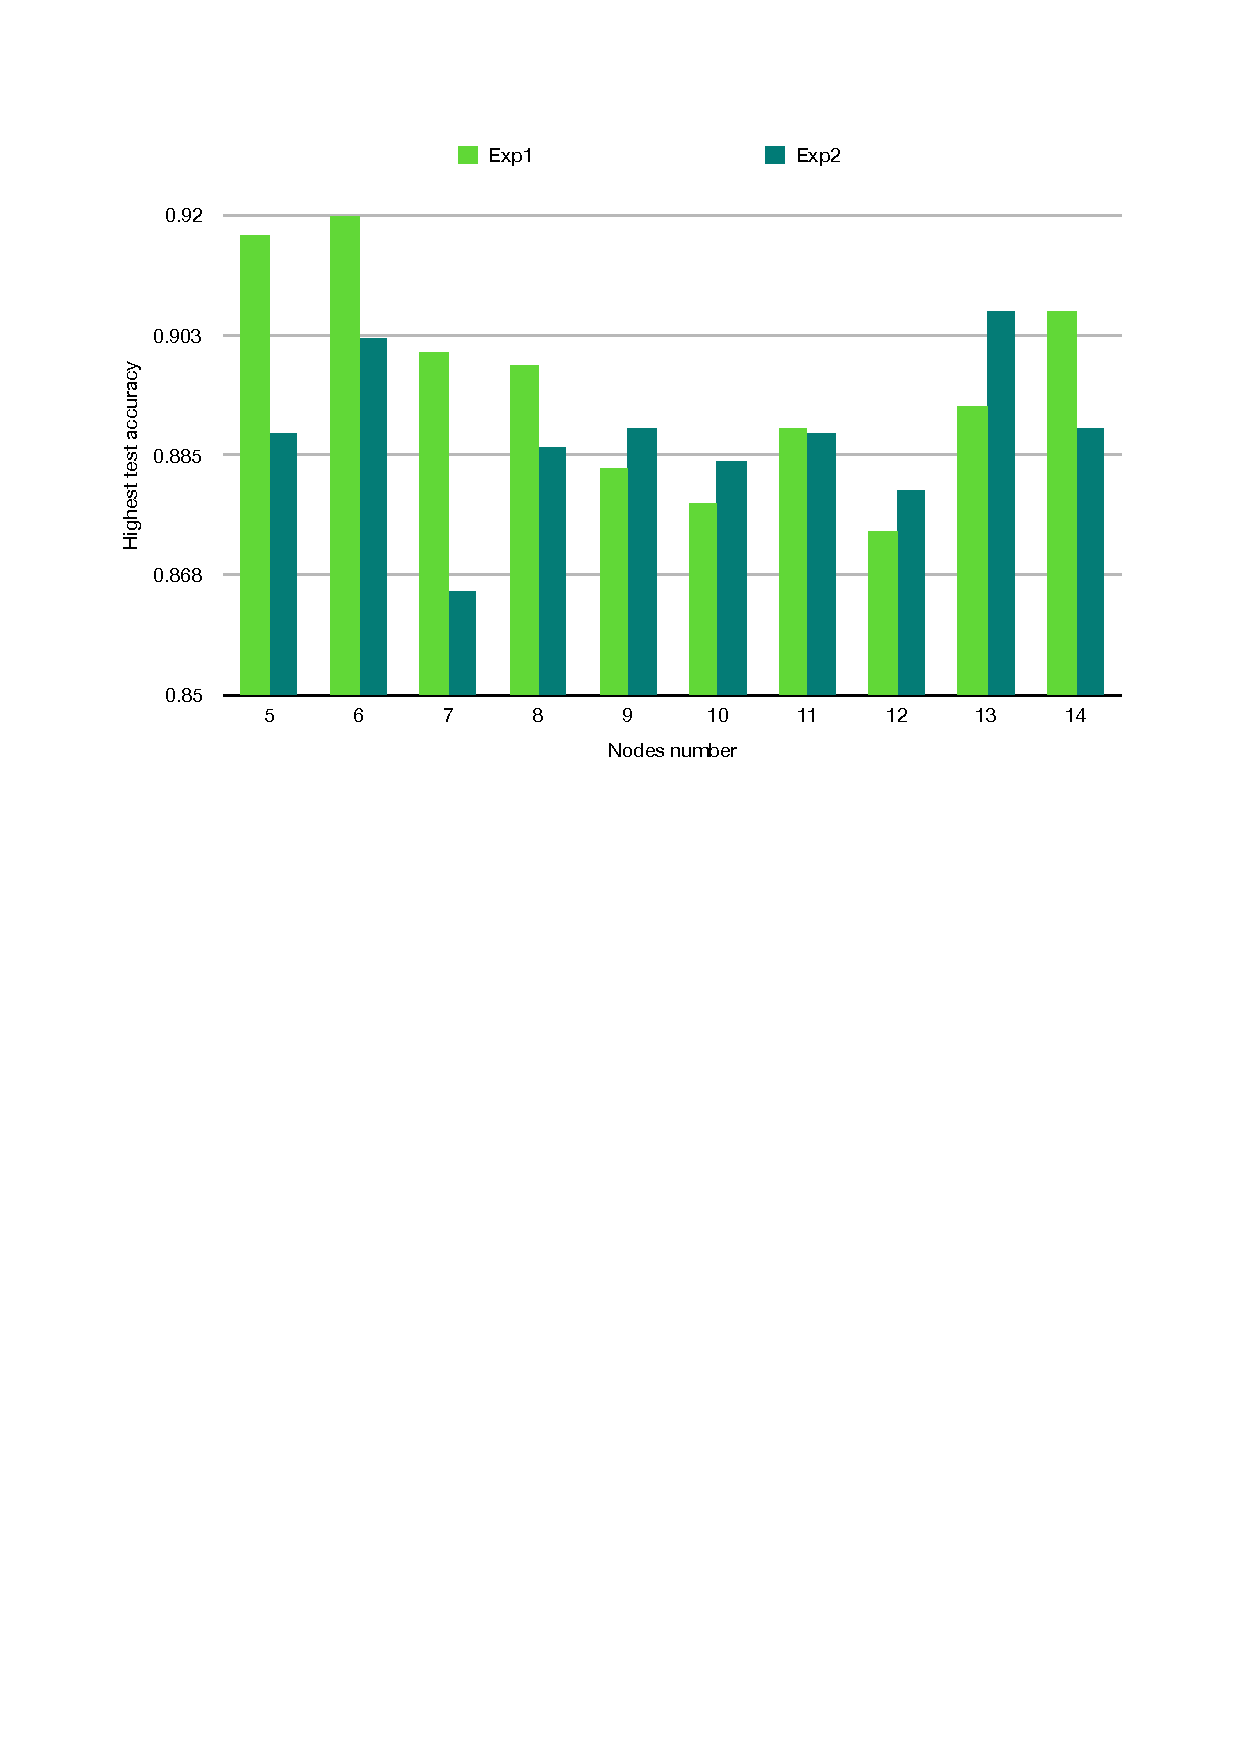
\includegraphics[width=\textwidth]{img/expdchart.pdf}
    \caption{Chart of test accuracy}
    \label{fig:expdchart}
\end{figure}





\section{Evaluation and Summary}
\label{sec:evaluation}

% This gives an evaluation of the project, including

% A description of how the project is evaluated, including
    % What criteria are used to evaluate whether the system is suceesful?
    % How these criteria are assessed?
    % Who is involved in the evaluation?
% Your critical evaluation of your project results/outcomes.
% Your critical evaluation of the strengths and weaknesses of your project as carried out.
% Where appropriate, 3rd party evaluation of the software/computer system/application developed on the project, and/or customer feedback, be obtained in strict accordance with
    % ethical use of the project 3rd party evaluation human participants
        % explicitly state if human participants were involved for the project 3rd party evaluation;
        % if human participants were involved for the project 3rd party evaluation,
            % explicitly confirm that the CS Department ethical procedure for Comp39x projects 3rd party evaluation has been followed.
            % include into appendix the 3rd party evaluator information sheet and consent forms completed and signed by the 3rd party evaluators on your project.

From the engineering aspect, the project is generally good and gives two command line application as research tools.
One can generate same scale graphs pairs with the bisimulation flag that ready to be used as data set for machine learning.
And the scale of the graph, number of pair, the rate of positive and negative, graph density can be customised.
Other can use the data generated to training a preset neural network.
In this tool, the number of training epoch, learning rate, batch size, the rate of test set and training set division can be customised.
And the training can be continued after the program ends.
The whole project was pushed as expected.
All components were tested and work well.
Nevertheless, the process of the project still needs improvement.
The most important is the test of components.
It was done by hand, which not reliable and inefficient.
Most test data from the textbook is reliable but not enough in quantity.


On the other hand, form aspect of research, the goal is generally achieved.
Whereas, it opens the next stage of research.
There are two experiments done in this project.
First is the wide experiment. 
It tests the performance of the learning algorithm when feeding the data (mainly) from different parts of space (i.e. all possible same scale graphs).
The experiment shows that in most situation the performance of the algorithm is similar.
Base on it, one can say that except the extreme situation (i.e. graph density equals 0.9) the performance of the algorithm when feeds a non-extreme value, is representative respect to the graphs pair with the same scale.
Second is the deep experiment.
It is aimed at testing the capability of the preset neural network.
It will test the performance of the learning algorithm when feeding the data with different scale (i.e. node number)
Base on the conclusion of the wide experiment, only the dataset generated with one density will be used to represent the result of the whole space in this very scale.
And the result shows that when the graphs become bigger, the performance did become worse,
which indicate the limitation of the neural network.
However, when the scale keeps expanding to a certain level, the performance unexpectedly become better.
It may be because of the insufficient quantity, but there still needs more experience.

Still, there are many things need to be improved as a research project.
Firstly, the literature review needs to be more at the begin of the project.
At the start of the project, most literature reviewed is about bisimulation.
The main aim was overlooked during the development of the first part.
It caused problems when the project stepped into the second part.
Some components need to be rewritten in order to serve the second part.
Second, the experiment design should be carefully considered.
For the wide experiment, the dataset used can be better by mixing all graphs pairs generated on different density then sampling from the pool.
For the deep experiment, the criteria of the deep experiment is quite blurred.
And the result indicates that more experiments are needed.

Moreover, for further experiments a better test cases generator may need to be designed.
The generator designed and implemented in the project aimed at ``random".
In other words, the generator was designed to be as random as possible.
However, in fact, true random generated graphs are mostly like the graphs shown in Figure \ref{fig:outputg3} and Figure \ref{fig:outputg4}.
They are either very easy to be denied or very simple to be recognised (see Section \ref{sec:results}).
Concretely, it is possible that 80\% of graphs pairs belongs to the above two types.
In that situation, the network will only need to learn to distinguish these two types of graphs, the performance can reach over 80\% accuracy while lacking generalisation ability.
Thu, the better idea may be a generator that can generate all kinds of pair while decreasing the incidence of these two types.
And generative adversarial network (GAN) can be a good choice.

\section{Learning Points}
\label{sec:learning}
% At least one page of summary of the key learning points in the project.
In this section all the materials and skill had been learning will be listed.
During the development of this project, many things had been learned, including the theories, programming skills and research skills.
\begin{itemize}
    \item \textbf{Theories}
    \begin{itemize}
        \item Bisimulation 
        \begin{itemize}
            \item Online Course: System Validation: Automata \& behavioural equivalences \cite{Groote2016}
            \item Thesis reading, about modal logic (e.g. \cite{VanBenthem1976,Blackburn2001a}), model checking (e.g. \cite{Roscoe1994}), bisimulation (e.g \cite{Glabbeek2011, Stirling2011a, Larsen1991}) and relevant algorithm (e.g. \cite{Paige1987, Dovier2004})
            \item Understand the bisimulation and the algorithm
        \end{itemize}
        
        \item Machine learning
        \begin{itemize}
            \item Online Course: Machine Learning by Andrew Ng \cite{Ng2015}
            \item Thesis reading, about neural network (e.g. \cite{Dayhoff1990}), machine learning on logic (e.g. \cite{holldobler1999approximating, Leshno2013})
        \end{itemize}
        
    \end{itemize}
    
    \item \textbf{Programming Skills}
    \begin{itemize}
        \item programming in \texttt{Python} with \texttt{PyCharm}
        \item Using \texttt{TensorFlow} to construct a neural network with visualisation, i.e. \texttt{TensorBoard}
        \item Using GPU to train the neural network
        \item Using package like \texttt{matplotlib, graphviz} to visualise the graphs
        \item Using \texttt{Git} and \texttt{Github} to manage the project
        \item Using remote computing server i.e. Google Cloud Platform
        \item Deploying experiments on \texttt{Linux}
        \item Using \LaTeX to typeset the dissertation
    \end{itemize}
    \item \textbf{Research Skills}
    \begin{itemize}
        \item Searching relevant thesis
        \item Reading, understanding and reproducing the algorithm of the thesis especially \cite{Paige1987}.
        \item Scheduling the project with Gantt-chat
        \item Analysis of information from different sources
    \end{itemize}
\end{itemize}
Nevertheless, except the skills had been learned.
There are also many skills that need to be improved or mastered.
The most important one is the skill to find the information.
At the first stage of the project, the research focus on the bisimulation. 
Meanwhile, the literature about the neural network on logical learning was not collected and reviewed sufficiently, which affected later study on machine learning.
The literature review should cover the whole project before actually working on it, rather than reviewing partially.


\section{Professional Issues}
\label{sec:profession}
% At least one page of discussion of how your project related to the codes of practice and conduct issued by the British Computer Society.
In this section the professional Issues base on the codes of practice and conduct issue by the British Computer Society will be discussed.

\subsubsection*{Technical Competence:}

At very first, trying to maintain the technical competence, all course provided by the university is taking. 
Further some extra online courses about the project like Machine Learning (see Section \ref{sec:learning}) and etc. has been taken during the project.
Also, before using the newly learned skill or some new design structure, it will be discussed during the regular meeting with the supervisor.
For example, the design scheme of the test case generator and the structure of the neural network were all discussed before actual implementation.

\subsubsection*{Public Interest:}
Data of this project did not involve any issue of public privacy, security and etc. directly.
All the data used here is self-generated abstract mathematical concepts. 
Any information related to intellectual property is annotated and used legitimately.
The softwares and libraries used either open source (e.g \texttt{TensorFlow}) or use free education version (e.g. \texttt{PyCharm}).

\subsubsection*{Duty to Relevant Authority:}
In the process of the project, the Relevant Authority's instruction is and will be respected and acted.
Section 9 of the Code of Practice on Assessment and University's Code of Practice is understood and acted honestly, ethically and professionally, during the whole process of the project.
Also, there is not any misrepresent information on the performance of any products involved in this project.

\subsubsection*{Duty to the Profession:}
Many pieces of literature relevant to the project had been read to maintain the specialism.
After the evaluation of this project, it is planned that the code of this project will be open-source under permission.
Thus, knowledge can be shared freely and support other researchers.




\newpage
\pagenumbering{roman}
\addcontentsline{toc}{section}{Appendices}
\appendix
\section{Appendices}
\label{sec:appendics}
% Appendices are meant to contain detailed material, required for completeness, but which are too detailed to include in the main body of the text. Typically they should contain code listings, details of test data, screen shots of sample runs, a user guide, full design diagrams, instructions for unpacking and mounting any software included with the dissertation and similar material. A zip file containing the project archive material (including source codes, instructions on how to run the software, pictures used, etc.) should be submitted through the E-project system. If your system is available on-line, you should provide instructions of how to access the system via the internet.

\subsection{User Manuel}
\subsubsection*{Installation}
To run these tools, the depend packages need to be installed.
\begin{minted}[frame=single,breaklines]{text}
$ pip install -r requirements.txt

\end{minted}
Notice that, it is recommend to installed in virtual environment.
\subsubsection*{Usage}

These tools is developed on \texttt{Python 2.7}.

For quick test, please run the command directly without any parameters.
\begin{minted}[frame=single,breaklines]{text}
$ python ml_algorithm/ml_algorithm.py
$ python standard_bisim/test_cases_generator.py
\end{minted}

To run the wide and deep experiments:
\begin{minted}[frame=single,breaklines]{text}
$ python experiments.py 
\end{minted}

Follows are specific direction:

\begin{minted}[frame=single,breaklines]{text}
$ python ml_algorithm/ml_algorithm.py -h

usage: ml_algorithm.py [-h] [-e EPOCH] [-l LEARNING_RATE] [-b BATCH_SIZE]
                       [-p DATA_PATH] [-r TEST_TRAIN_RATE] 
                       [-c CONTINUE_TRAIN] [-n MODEL_NAME]

optional arguments:
  -h, --help            show this help message and exit
  -e EPOCH, --epoch EPOCH
                        Number of training epochs
  -l LEARNING_RATE, --learning_rate LEARNING_RATE
                        Initial learning rate
  -b BATCH_SIZE, --batch_size BATCH_SIZE
                        Number of data for one batch
  -p DATA_PATH, --data_path DATA_PATH
                        Path to input data
  -r TEST_TRAIN_RATE, --test_train_rate TEST_TRAIN_RATE
                        The rate of test cases and train cases
  -c CONTINUE_TRAIN, --continue CONTINUE_TRAIN
                        Continue last training
  -n MODEL_NAME, --model_name MODEL_NAME
                        The name of the model
\end{minted}
\begin{minted}[frame=single,breaklines]{text}
$ python standard_bisim/test_cases_generator.py -h

usage: test_cases_generator.py [-h] [-t {random,all}] [-n NUMBER]
                               [-f FILE_NAME] [-v NODE_NUMBER]
                               [-e EDGE_TYPE_NUMBER] [-r P_RATE]
                               [-p PROBABILITY]

optional arguments:
  -h, --help            show this help message and exit
  -t {random,all}, --type {random,all}
                        Type of data set
  -n NUMBER, --number NUMBER
                        The length of data set
  -f FILE_NAME, --file_name FILE_NAME
                        Name of the output file
  -v NODE_NUMBER, --node_number NODE_NUMBER
                        Number of the nodes of the graph in the data set
  -e EDGE_TYPE_NUMBER, --edge_type-number EDGE_TYPE_NUMBER
                        The total types of the edge in the graphs
  -r P_RATE, --p_rate P_RATE
                        Rate of the positive cases over all cases
  -p PROBABILITY, --probability PROBABILITY
                        The density of the random generate graphs
\end{minted}

Here is the directory tree of the whole project.

\begin{minted}[frame=single,breaklines]{text}
FYP
    Bisimulation_fyp_2019
        experiments.py
        ml_algorithm
        requirements.txt
        standard_bisim
    FYP_report
        img
        main.tex
        reference.bib
        tex
    experiment_data
        deep
        wide
\end{minted}

To visulise the performance of machine learning please use \texttt{TensorBoard}
\begin{minted}[frame=single,breaklines]{text}
$ tensorboard --logdir <path-to-summary-folder> --host localhost
\end{minted}
\newpage
\addcontentsline{toc}{section}{References}
\bibliographystyle{ieeetr}
\bibliography{reference}

\end{document}
